%%---------------------------------------------------------------------------%%
%% Draco Build System
%% draco_bs.tex
%%---------------------------------------------------------------------------%%
\documentclass[reqno]{larep}
%\usepackage[dvips]{graphicx}
%\usepackage{epsfig}
\usepackage{graphicx}
\usepackage{cite}
\usepackage[centertags]{amsmath}
\usepackage{amssymb}
\usepackage[mathcal]{euscript}
\usepackage{latexsym}
\usepackage{tmath}
\usepackage{c++,fancycodes}
\usepackage{tabularx}
\usepackage{draco_bs}
\usepackage{alltt}
%\usepackage{doublespace}
%\usepackage[nomarkers]{endfloat}
\usepackage{subfig}
\usepackage{hyperref}
\usepackage{listings}
\usepackage{color}
% \usepackage[colorlinks]{hyperref}
\usepackage{longtable}

\definecolor{listingBG}{rgb}{0.95,0.95,0.95}
\definecolor{inverse}{rgb}{0,0,0}

%% \lstset{language=C++,
%%         showstringspaces=false,
%%         frame=shadowbox,
%%         basicstyle=\footnotesize,
%%         rulesepcolor=\color{black},
%%         backgroundcolor=\color{listingBG}}

%\hypersetup{
%    %bookmarks=true,         % show bookmarks bar?
%    %bookmarksopen=true,     % show the bookmarks bar
%    unicode=false,          % non-Latin characters in Acrobat’s bookmarks
%    pdftoolbar=true,        % show Acrobat’s toolbar?
%    pdfmenubar=true,        % show Acrobat’s menu?
%    pdffitwindow=false,     % window fit to page when opened
%    %pdfstartview={FitH},    % fits the width of the page to the window
%    %pdftitle={My title},    % title
%    %pdfauthor={Author},     % author
%    %pdfsubject={Subject},   % subject of the document
%    %pdfcreator={Creator},   % creator of the document
%    %pdfproducer={Producer}, % producer of the document
%    %pdfkeywords={keyword1} {key2} {key3}, % list of keywords
%    pdfnewwindow=true,      % links in new window
%    colorlinks=false,       % false: boxed links; true: colored links
%    linkcolor=cyan,         % color of internal links
%    citecolor=green,        % color of links to bibliography
%    filecolor=magenta,      % color of file links
%    urlcolor=blue           % color of external links
%}

\makeindex

%%---------------------------------------------------------------------------%%
%% BEGIN DOCUMENT
%%---------------------------------------------------------------------------%%

\begin{document}

%%---------------------------------------------------------------------------%%
%% Front Matter
%%---------------------------------------------------------------------------%%

\frontmatter

\title{The Draco Build System}
\author{K.G. Thompson$^a$}
\address{$^a$CCS--2, MS D409, Los Alamos National Security, LLC, Los Alamos, NM 87545}
\email{kgt@lanl.gov}

\author{T.M. Evans$^b$}
\address{$^b$currently at ORNL}

\author{R.M. Roberts$^c$}
\address{$^c$D--6, MS F609, Los Alamos National Security, LLC, Los Alamos, NM 87545}
\email{rsqrd@lanl.gov}

\subjclass{CCS--2:12--43(U)}%, LA--12--NNNNN}
\date{\today}

\keywords{svn, make, GNU, cmake, ctest, cdash, compilers, g++, build system}

\begin{abstract}
  
  The Draco build system is designed to facilitate both development and
  usage on multiple platforms and using multiple build tools.  Originally, the build system adopted much of the GNU
  Coding Standards~\cite{gnu} for software packages.  However, as of 2011, the build system no longer relies on the GNU \soft{autotools} \index{autotools} and it supports non-Linux build platforms. While the design of the \draco\ build system is moving away from strict conformance to the GNU Coding Standards, it has been
  designed according to the following list of requirements:
  \begin{enumerate}
  \item support for simultaneous, multiple configurations (Release, Debug, etc);
  \item support for multiple programming languages.  The primary
    language is \cpp\ but support for for \lang{C} and \lang{Fortran}
    is required for all current ASC platforms.
  \item support for multiple build project types (\soft{Makefiles},
    \soft{XCode}, \soft{Eclipse}, etc.)
  \item the ability to support multiple code projects;
  \item support for external vendors;
  \item support for explicit template instantiation;
  \item \lang{C} and \cpp\ coding must conform strictly to issued ISO standards.
%\begin{enumerate}
%\item \cpp 03, also known as the ISO/IEC 14882:1998 standard amended by the 2003 technical corrigendum, ISO/IEC 14882:2003.
%\item \lang{C99}, also known as the ANSI C ISO/IEC 9899:1999 standard
%\end{enumerate}
  \item extensibility;
  \item low-cost on developers to add new packages, code, and tests; 
%  \item adoption of selected sections of the GNU coding standard \cite{gnu}.
%\begin{enumerate}
%\item \S4.2 Writing robust programs
%\item \S4.3 Library behavior
%\item \S4.4 Formatting error messages
%\item \S4.5 Standards for interfaces generally
%\item \S4.7 Standards for command line interfaces
%\item \S4.11 Memory usage
%\item \S4.12 File Usage
%\item \S5 Making the best use of \lang{C}
% We don't follow these items from GNU coding standards
% only use C and Posix.
% 4.1 Non-GNU standards
% 4.6 Standards for Graphical Interfaces
% 4.8 Standards for dynamic plug-in interfaces
% 4.9 Table of long options
% 4.10 OID Allocations
% 6 Documentation (We do use ChangeLogs)
% 7 Release process (no longer use configure, no longer require make)
%% 8 References to Non-Free Software (we referency many commercial or protected software/documentation)
%\end{enumerate}
  \item support for on-demand and automated regression testing with
    web-based dashboard presentation.
\item  preconfigured development environment for ASC platforms (\comp{bashrc/cshrc}, \comp{elisp}, vendors, extensions to the \soft{module} command, etc.)
%  \item support for \dejagnu\ and regression testing;
%  \item support for \purify;

  \end{enumerate}
  These requirements plus additional features such as
  threaded/parallel building, heterogeneous architectures and vendor
  support have been included in the \draco\ build system.
  
  The build system primarily uses three CMake tools~\cite{cmake},
  \cmake, \ctest and \cdash.  Version control of the \draco\ source is
  performed by \svn~\cite{svn-redbean}. These tools are freely
  available from \href{http://kitware.com}{Kitware} and
  \href{http://tigris.org}{Tigris.org}, respectively.

%
%\vspace{0.5in}

  %% The build system uses four GNU tools, \autoconf, \gmake, \gmfour,
  %% and \dejagnu.  Version control of the \draco\ source is performed by
  %% \cvs.  These tools are all freely available from the Free Software
  %% Foundation.

\end{abstract}
\maketitle

\tableofcontents
\listoffigures
\listoftables
% \lstlistoflistings % [KT 4-17-2012 This isn't working for me]

%%---------------------------------------------------------------------------%%
%% Main Matter
%%---------------------------------------------------------------------------%%

\mainmatter

%%---------------------------------------------------------------------------%%
%% introduction for imc-dev manual
%%---------------------------------------------------------------------------%%

\section{Introduction}

The \imctest\ package represents a first step towards the development
of \milagro.  In this sense, \imctest\ may be considered an early
release of \milagro.  The goals of \imctest\ are:
\begin{enumerate}
\item develop an extensible \C++ object-oriented/generic design;
\item test the implementation of the IMC algorithm on several simple
  test problems;
\item test the parallel performance of IMC on several platforms.
\end{enumerate}
The object-oriented/generic design of \imctest\ will ensure an easy
transition to the full \milagro\ package.  The improvements and
additions that are required to promote \imctest\ to \milagro\ include:
\begin{enumerate}
\item interfaces to various host-codes;
\item improved physics;
\item new mesh-types and geometries;
\end{enumerate}
The classes and data structures in \imctest\ are easily extensible;
thus, the classes used in \imctest\ should work in \milagro. For more
information, the \jayenne\ code development plan is described in
detail in Ref.~\citen{xtm:rn98xxx}.

The purpose of this manual is to document the code structure of the
\imctest\ package for users of the \imctest\ library.  In essence, this
manual contains the following information:
\begin{itemize}
\item a listing and description of the classes and data structures
  which comprise the \imctest\ library;
\item descriptions of the interactions between classes and types in
  \imctest;
\item descriptions of the interfaces for each class in \imctest.
\end{itemize}
The information presented herein will facilitate easy usage of the
\imctest\ library by code developers in X-division.  It will also serve
as a reference for users of the code.



%%---------------------------------------------------------------------------%%
%% model.tex 
%% description of the draco component library and overview of the build system
%% ---------------------------------------------------------------------------%%

\chapter{The Draco Model}
\label{chap:model}

This chapter presents an overview of the \draco\ build model, architecture and
source.  We present, in detail, the requirements for the \draco\ build
system in \S~\ref{sec:build_sys_req}.  Because the \draco\ build model
was originally designed to conform to the GNU coding standard, a brief
summary of GNU requirements is given in \S~\ref{sec:gnu_build_model}.
Finally, this chapter concludes with a description of the \draco\ 
source tree and files that are created during configuring and
building.

%%---------------------------------------------------------------------------%%

\section{Overview of Draco}
\label{sec:overview_of_draco}

Documentation describing the purpose and capabilities of packages
within \draco\ is beyond the scope of this text.  However, a brief
summary of \draco\ is pertinent to this discussion.  \draco\ is a
component library for computational radiation transport.  \draco\ is
primarily a \cpp\ library; however, other language support is not
precluded in \draco.  In particular, \draco\ has plans to support \lang{ISO\_C\_BINDING} interfacing between \cpp\ and \fortran.  A more general type of 
automatic type-interfacing between \cpp\ and \fortran~\cite{gr99} was implemented to support \sys{Dante} code, but was abandoned in favor of a simpler interface paradigm.
% Additionally, we plan to incorporate a generalized interface for
%problem input specifications using \python\ extensions.

The products of \draco\ are individual component libraries
that provide reusable services geared towards radiation transport
applications.  For example, \draco\ provides random number generators that may be used by a Monte
Carlo radiation transport solver.  \draco\ also provides access to opacity models and an angular quadrature component that can be used by deterministic radiation transport solvers.  In addition to components designed for radiation transport,
\draco\ provides several service packages including \dsxx, a data
structures library that contains numeric containers, smart pointers,
and assertions, and \cfour, a communications library, among others.

%The fundamental principle guiding code design in \draco\ is templating
%on Mesh Types (MT).  Thus, the libraries in \draco\ will work with any
%code that provides a MT with the proper services.  This allows highly
%efficient implementations of various meshes to be included in generic
%radiation transport packages.  

\draco\ is designed using object-oriented~\cite{me97} \index{object-oriented}and generic
programming~\cite{au99} \index{generic programming} philosophies.  Foremost among these notions
are levelized design \index{levelized}, Design-by-Contract$^{\text{\footnotesize TM}}$, \index{ Design-by-Contract}
and the generic concept-model idea.  Other software engineering
methods are employed for quality control including regression testing,
automatic documentation, code profiling, and design and code reviews.

  

%%---------------------------------------------------------------------------%%

\section{Overview of the Draco Build Model}
\label{sec:overview_draco}

\subsection{Software Requirements}

Originally, the \draco\ build system was designed according to the GNU coding
standard and made use of  \autoconf~\cite{autoconf},
\gmake~\cite{gmake}, and \gmfour~\cite{m4} for configuring and building components.  
In 2011, this requirement was altered as the development team chose to replace the
aging build system with a \cmake-based system~\cite{cmake}.  In addition, \draco\ version
control is performed by \svn~\cite{svn-redbean}.  

Additional software is used for performing quality control.
Regression testing is handled by \cmake's \ctest\ and \cdash\ tools.  Bugs are
tracked using \teamforge~\cite{teamforge,teamforge-lanl}.  In addition, an archived email
list is available to submit design plans and discussion between team
members.  Also, \valgrind~\cite{valgrind}, \bullseye~\cite{bullseyeweb} and \cloc~\cite{clocweb} play important roles in the
quality control process.  The build system supports
processing code and tests through \valgrind\ on all platforms for performing dynamic memory and cache analysis. It supports the use of \bullseye\ for analyzing \cpp\ code coverage metrics (function and condition/decision branch coverage) and it uses \cloc\ for tracking total lines of source code.  All of this information is collected nightly by the regression system and published on the \draco\ regression dashboard at \url{http://coder.lanl.gov/cdash}.
 
The \draco\ build system contains support for multiple language
environments.  However, the primary language in use at present is the 1998 ANSI
Standard \cpp~\cite{ansi:cpp}.  \draco\ does not currently support the 2011 ANSI \cpp\ Standard~\cite{ansi:cpp11}\index{C++ 2011} because LANL standard compiler's do not support the new standard yet.  As soon as the required compilers support the new standard, \draco\ will allow code to be written that conforms to the 2011 standard. Currently, any \cpp\ compiler that conforms to the 1998 standard will compile \draco.  Portland Group, Intel and GNU \cpp\ are regularly used for building on ASC hardware. 
Currently, there
is no \fortran\ code in \draco; although, we expect that to change in
the future.  (The build system does look for a \fortran\ compiler during the configuration step so that a compatible version of LAPACK can be located and tested with the selected linker.)
Additional languages required by \draco\ are \python\ and 
\lang{PERL}.  \draco\ expects these scripting
languages to be located in a directory that is included int he developer's \comp{PATH},
and the build system checks for this.   A suite of tools that can typeset \LaTeX\ sources is also
necessary for compiling much of the documentation that comes with \draco.
  
%   Unfortunately, the Kuck and Associates
%\cpp\ compiler, \soft{KCC}~\cite{kai}, is the only ANSI Standard
%compatible compiler on the market today.  Thus, \soft{KCC} is required
%to compile \draco\ in its entirety. \soft{KCC} is available on all
%platforms of interest to Los Alamos National Laboratory and the
%Accelerated Strategic Computing Initiative (ASCI).  

With the exception of \bullseye\ and the listed commercial compilers, all of the
aforementioned software products are freely available.  Note that \bullseye\ is mainly a
development tool and is not required to configure, build, or use
\draco.  Also note that the GNU set of compilers is freely available and using them allows \draco\ to be built without the use of any commercial software.

The build system checks for the presence of each of aforementioned software products; thus, as
long as the software is in the user's path, the configuration will
succeed.  Finally, \draco\ utilizes a number of vendor libraries,
depending upon configuration, that must be installed on the system in
which \draco\ resides.  Detail on these packages and their
configuration options is given in Chap.~\ref{chap:compile}.

\begin{table}
  \begin{center}
    \caption{Required and optional tools for configuring and building \draco.}
    \label{tab:reqtools}
    \begin{tabular}{lp{1.5in}p{1.5in}p{1.5in}}\hline\hline
    
          Tool & Required  & Recommended & Optional \\ \hline
	Configuration & \cmake-2.8.6+ & \ctest & \cdash  \\
	\cpp\ compiler & Any standards compliant \cpp\ compiler &  g++ 4.5 & Intel 10-12, PGI 11 \\
	\fortran\ compiler & optional & gfortran 4.5+ & Intel 10-12, PGI-11 \\
	Build tool & any of ... & \gmake & Eclipse CDT, XCode, Visual Studio \\
	Scripting language & \cmake & \python & \perl \\
	Version control & \svn & & \git \\
	Dynamic Analysis & optional & \valgrind & \\
	Code Coverage & optional& \bullseye & \\
	Lines-of-Code & optional & \cloc & \\
	Bug Tracking & optional & \teamforge & ChangeLog, text files, email \\
	Documentation & optional & \LaTeX\ typesetting tool, \doxygen & \\	
	\hline \hline

    \end{tabular}
  \end{center}
\end{table}



\subsection{Build System Requirements}
\label{sec:build_sys_req}

In \S~\ref{sec:purpose} the requirements that guided the development
of the \draco\ build system were summarized.  In this section, we
shall take an expanded look at the complete list of requirements.  The
list of requirements for the \draco\ build system is:
%
\begin{enumerate}
\item support for simultaneous, multiple configurations (Release, Debug, Scalar, Parallel, etc);
\item support for multiple programming languages, while preferring \lang{C} and \cpp;
\item support for \cpp\ on all current ASC platforms;
\item \lang{C} and \cpp\ coding must conform strictly to issued ISO standards~\cite{ansi:cpp} \index{ISO standard}:
\begin{enumerate}
\item \cpp 03, also known as the ISO/IEC 14882:1998 standard amended by the 2003 technical corrigendum, ISO/IEC 14882:2003;
\item \lang{C99}, also known as the ANSI C ISO/IEC 9899:1999 standard;
\end{enumerate}
\item support for multiple build project types (\soft{Makefiles}~\cite{gmake}, \soft{XCode}, \soft{Eclipse}, etc.)
\item on-demand and automated unit and regression testing; \index{regression testing}
\item support for \cdash~\cite{cmake,codercdash} presentation of regression results;
\item support for \valgrind~\cite{valgrind} dynamic analysis integrated into \cdash\ presentation; \index{valgrind}
\item the ability to support multiple code projects;
\item extensible support for external vendors; 
\item support for explicit template instantiation; \index{explicit template instantiation}
\item extensibility;
\item low-cost on developers to add new packages, code, and tests; 
\item  adoption of selected sections of the GNU coding standard~\cite{gnu} \index{GNU
    Coding Standard}.
\end{enumerate}
%
We will analyze each of these requirements in turn.  First, from a
development standpoint, having multiple configurations at the same
time is a must.  This feature is required because certain tools work
better on certain platforms.  Additionally, certain tools work better
in certain environments.  For example, we often require both scalar
and parallel versions of the code for profiling and testing.  The
\draco\ build systems allow each configuration, and the products it
produces, to exist in a unique directory.  Thus, builds are not
performed in the source code tree; they are done in a user-specified
directory.  More detail is given on multiple configurations and builds 
in \S~\ref{sec:draco_src_tree} and Chap.~\ref{chap:compile}.

% #2
\draco\ is not a single language system.  Although \draco\ is
presently composed of \cpp\ code, we expect multiple languages
(in particular \lang{Fortran}) to be supported for interfacing and numerical
optimization.  The \draco\ build system is general and is not
restricted to single language support.  Supporting multiple languages
is an essential requirement because \draco\ customers utilize many
frameworks and languages.

% #3 & #4
\cpp\ source code in \draco\ must conform to the the ISO/IEC 14882:1998 standard amended by the 2003 technical corrigendum, ISO/IEC 14882:2003. \index{ISO standard} This ensures that \cpp\ sources will 
compile by any standards compliant \cpp\ compiler.  The DBS activates many compiler warning flags for Debug builds so that developers are notified if their code deviates from the standard.  In particular, code that does not compile cleaning using ASC standard compilers on target ASC platforms must be brought into compliance or be removed from the \draco\ system.

% #5
In recent years the need to support non-command line integrated development environments, \index{integrated development environment} IDE, has become increasingly important.  With the conversion of the build system from \soft{autotools} to \cmake\ in 2011, this has become a build system requirement.  The primary build tool continues to be \soft{Makefiles} but support for the \soft{Eclipse CDT} IDE on Linux and for the \soft{XCode} IDE on OS/X is also supported.

% #6-#8
The next three requirements are aimed at \draco\ system and package
developers and are essential for developing high quality software.
%  The \draco\ build system must support \dejagnu.  
Regression and unit testing are an important part of the \draco\ quality assurance program.  \draco\ developers must have the ability to run a test suite to determine if local changes adversely impact other parts of the \draco\ system.  The daily
testing of \draco\ components also ensure that commits to
one part of the library do not adversely affect other components.  These daily tests are run on multiple platforms and may catch coding issues that only appear on specific hardware/software combinations.  The results from nightly testing must be published to the \draco\ Dashboard~\cite{codercdash} and email sent to developer who request nightly updates.  Additionally, code coverage metrics by \bullseye, dynamic analysis (via \valgrind) and lines-of-code metrics must also be collected nightly so that the time evolution of issues can be tracked and to allow the \draco\ development team the data needed to target specific improvements.  Such improvements might be the addition of unit tests so that more baseline code is checked in the nightly tests or the elimination of memory errors.

% #9
In addition to being self supportive, the \draco\ build system will be designed to be exported to other code projects.  This requirement includes the ability of other code projects to use build system scripts found in \draco\ and the ability to find and link against \draco\ code and vendor code known by by \draco.  The \sys{Capsaicin} and \sys{Jayenne} code projects both employ the \draco\ build system and also link to \draco\ component libraries.

% #10
As a suite of scientific simulation tools, \draco\ components often need to link against vendor software to provide specialized capabilities.  For example, most of \draco\ is designed to be run in parallel under MPI.  MPI is a vendor tool supported by \draco.  The build system can detect the local availability of MPI and will adjust build parameters based on the flavor and version of MPI.  For example, if MPI is not found on the local system, the build system automatically switches to \comp{SCALAR} mode and does not attempt to link libraries and executables against the MPI libraries.  While \draco\ can be built without MPI, it is assumed to be a required vendor in most cases.  The GNU Scientific Library is also considered to be a required vendor for \draco\ as it provides random number generation  features and many linear algebra functions.  Optional vendors for \draco\ include BLAS, LAPACK, ScaLAPACK, BLACS, Trilinos and xmgrace among others.  Extending the \draco\ build system to support other vendors is straight forward and transparent.

% #11
A guiding principle of the \draco\ build system is explicit template
instantiation. \index{explicit template instantiation}  We have found that this provides a  more robust
and efficient build system compared to the environment where the compiler is allowed to
instantiate template classes and functions {\it automatically}.  The essence of explicit
instantiation is that the package developer determines what templated classes
are instantiated (and when they are instantiated)~\cite{cpptemplates}.  \draco\ does not implicitly
instantiate template classes and functions.  \draco\ has rules on how
template classes and functions are explicitly instantiated.  These are
listed in Chap.~\ref{chap:adding}.  Additional information for clients
that use \draco\ class and function templates is listed in
\S~\ref{sec:using}.

% #12 - #13
Another guiding principle of the \draco\ suite of components is the concept that active features are constantly changing.  New features are regularly added to \draco\ and deprecated features are removed periodically.  It is imperative that the DBS flexibly support these changes so that the developer cost of adding or removing components remain low.   This is accomplished through the encapsulation paradigm and the levelized component design of \draco.  The DBS itself must remain extensible as new requirements for the build system come into play.

% #14

The final requirement is that the \draco\ build system should continue to adhere to the GNU Coding Standard~\cite{gnu} as much as is reasonable.  Obviously, the adoption of \cmake\ and non-Makefile based build systems is not supported by this standard and we have made a deliberate decision to make the build system more flexible at the cost of standardization.  By formalizing our build model on an accepted standard, we reduce the overhead associated with maintaining the system. In the case of the \cmake-based build system, we make heavy use of the features provided by \cmake\ and avoid the use of custom build scripts except for cases that are absolutely necessary (i.e.: python scripts for running application codes and checking the results against gold standards).  A summary of the pertinent parts of the GNU standard is given in \S~\ref{sec:gnu_build_model}

\subsection{The GNU Build Model}
\label{sec:gnu_build_model}

A full description of the GNU Coding Standards is beyond the scope of
this text.  Interested readers are referred to Ref.~\cite{gnu} for
more information.  However, a brief summary of the pertinent aspects
of the coding standard is useful here.  As we have previously
mentioned, the \draco\ build system corresponds to the guidelines set
forth in the GNU standard.  The relevant parts of the GNU standard
that affect \draco\ are the sections pertaining to documentation and
program release.  We shall look at these in turn.

The GNU standard specifies the following requirements on release
documentation:
\begin{enumerate}
\item provide a manual describing the system using \soft{texinfo}, this can refer to other documentation;
% \item a \comp{NEWS} file should contain highlighted, version update information;
\item a \comp{ChangeLog} file should contain a log of changes made to the product between different releases;
\item man pages are optional.
\end{enumerate}
\draco\ does not presently have man pages, and no attempts are
underway to make them.  The other requirements are met with the
following exceptions: \draco\ uses \LaTeX\ and \doxygen\ for its documents and
contains more than one manual due to its size and multiple uses.

\subsection{The CMake Build Model}
\label{sec:cmake_build_model}

The GNU standard specifies many constraints on build and make systems including a mandate to use  \comp{configure*} scripts and standardized configure options and \comp{Makefile} targets.  The \cmake-based \draco\ build system no longer makes any attempt to support these requirements.  Instead, the following build system features must be supported:
\begin{enumerate}
\item \cmake\ will be used to configure code products;
\item Each directory in the build system will have a \comp{CMakeLists.txt} file that describes local build targets, platform checks, and local testing instructions.
\item \cmake\ guarantees certain names (e.g.: \comp{PROJECT\_NAME}, \comp{PROJECT\_BINARY\_DIR}, \comp{CMAKE\_<LANG>\_FLAGS, \comp{MPI\_FOUND}, etc.}) to exist in the build.  A more complete list can be obtained by running '\comp{cmake --help-variable-list}.'
\item \cmake\ guarantees certain build project targets will be defined:
\begin{itemize}
\item all - generate all normal targets
\item clean - remove generated files (libraries, object files, binaries, etc.)
\item Experimental - run the build and tests and submit the results to the dashboard.
\item install - copy built files to the \comp{CMAKE\_INSTALL\_PREFIX} directory 
\item test -  run the unit tests
\item uninstall - remove files copied as a result of the install target
\end{itemize}
\item The DBS standardizes additional Makefile targets:
\begin{itemize}
\item Lib\_$<$component$>$
\item  Lib\_$<$component$>$\_test
\item Ut\_$<$component$>$\_$<$testname$>$\_exe
\end{itemize}
\end{enumerate}
Because \cmake\ does not restrict the build project to \soft{Makefiles}, we don't speak explicitly about {\it Makefile targets} and instead use the term {\it build targets}.  In general, the \draco\ build system attempts to use the same variable naming conventions as \cmake.

%\begin{enumerate}
%\item \comp{configure*} scripts should be used to configure code products;
%\item hardware and software options should be controlled by the
%  \comp{--with-\textsl{feature}} or \comp{--enable-\textsl{feature}}
%  command-line specifications to \comp{configure*};
%\item standard makefile services and targets are defined.
%\end{enumerate}
%Because \draco\ uses \autoconf\ to produce \comp{configure*} scripts,
%the first two requirements are met by default.  With regard to
%makefiles, the GNU standard specifies a lengthy list of required
%targets, definitions, and acceptable utilities.  \draco\ meets all of
%these requirements.  The one exception is that \draco\ is primarily a
%\cpp\ system.  This would seem to be in violation of the GNU standard.
%However, because of the specificity of the \draco\ client base, we are
%justified in using \cpp\ as described in \S~3.4 of the GNU Coding
%Standard.

%%---------------------------------------------------------------------------%%

\section{The Draco Source Code Tree}
\label{sec:draco_src_tree}

\subsection{Draco Source Tree}

In this section we give an overview of the \draco\ source tree. The
\draco\ source tree is illustrated in Fig.~\ref{fig:src_draco}.  The
subdirectories are in \index{source tree}
\begin{figure}
  \centerline{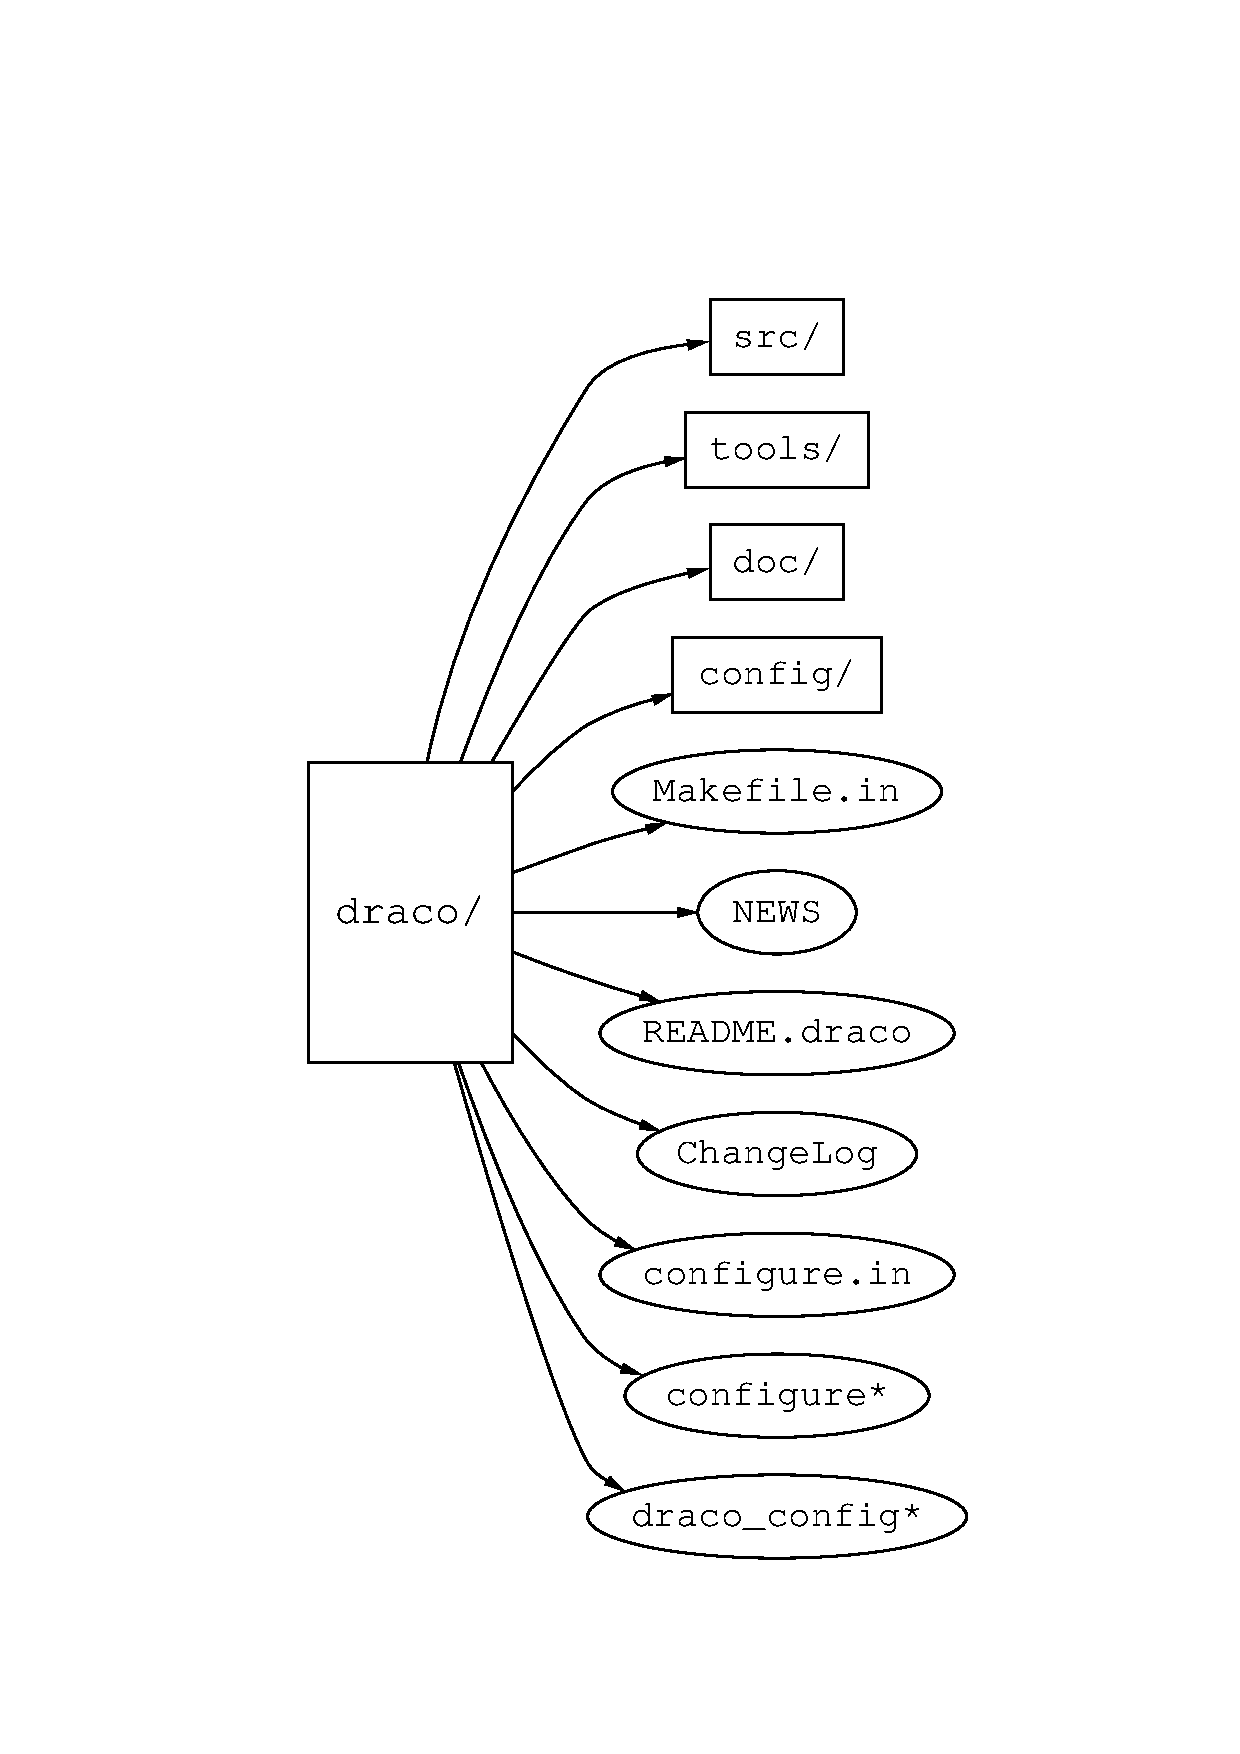
\includegraphics[clip,trim=1cm 4cm 1cm 4cm,width=3.5in]{fig/src_draco}} % [width=2in]
  \caption{The \draco\ source tree.  Directories are in boxes and
    files are in ellipses.  The subdirectories are shown in
    Fig.~\ref{fig:subdraco}.}
  \label{fig:src_draco}
\end{figure}
Figs.~\ref{fig:subdraco}a through c.  Note that these figures show the
\begin{figure}
  \begin{center}
    \begin{tabular}{ccc} 
      \subfloat[\comp{src/}]{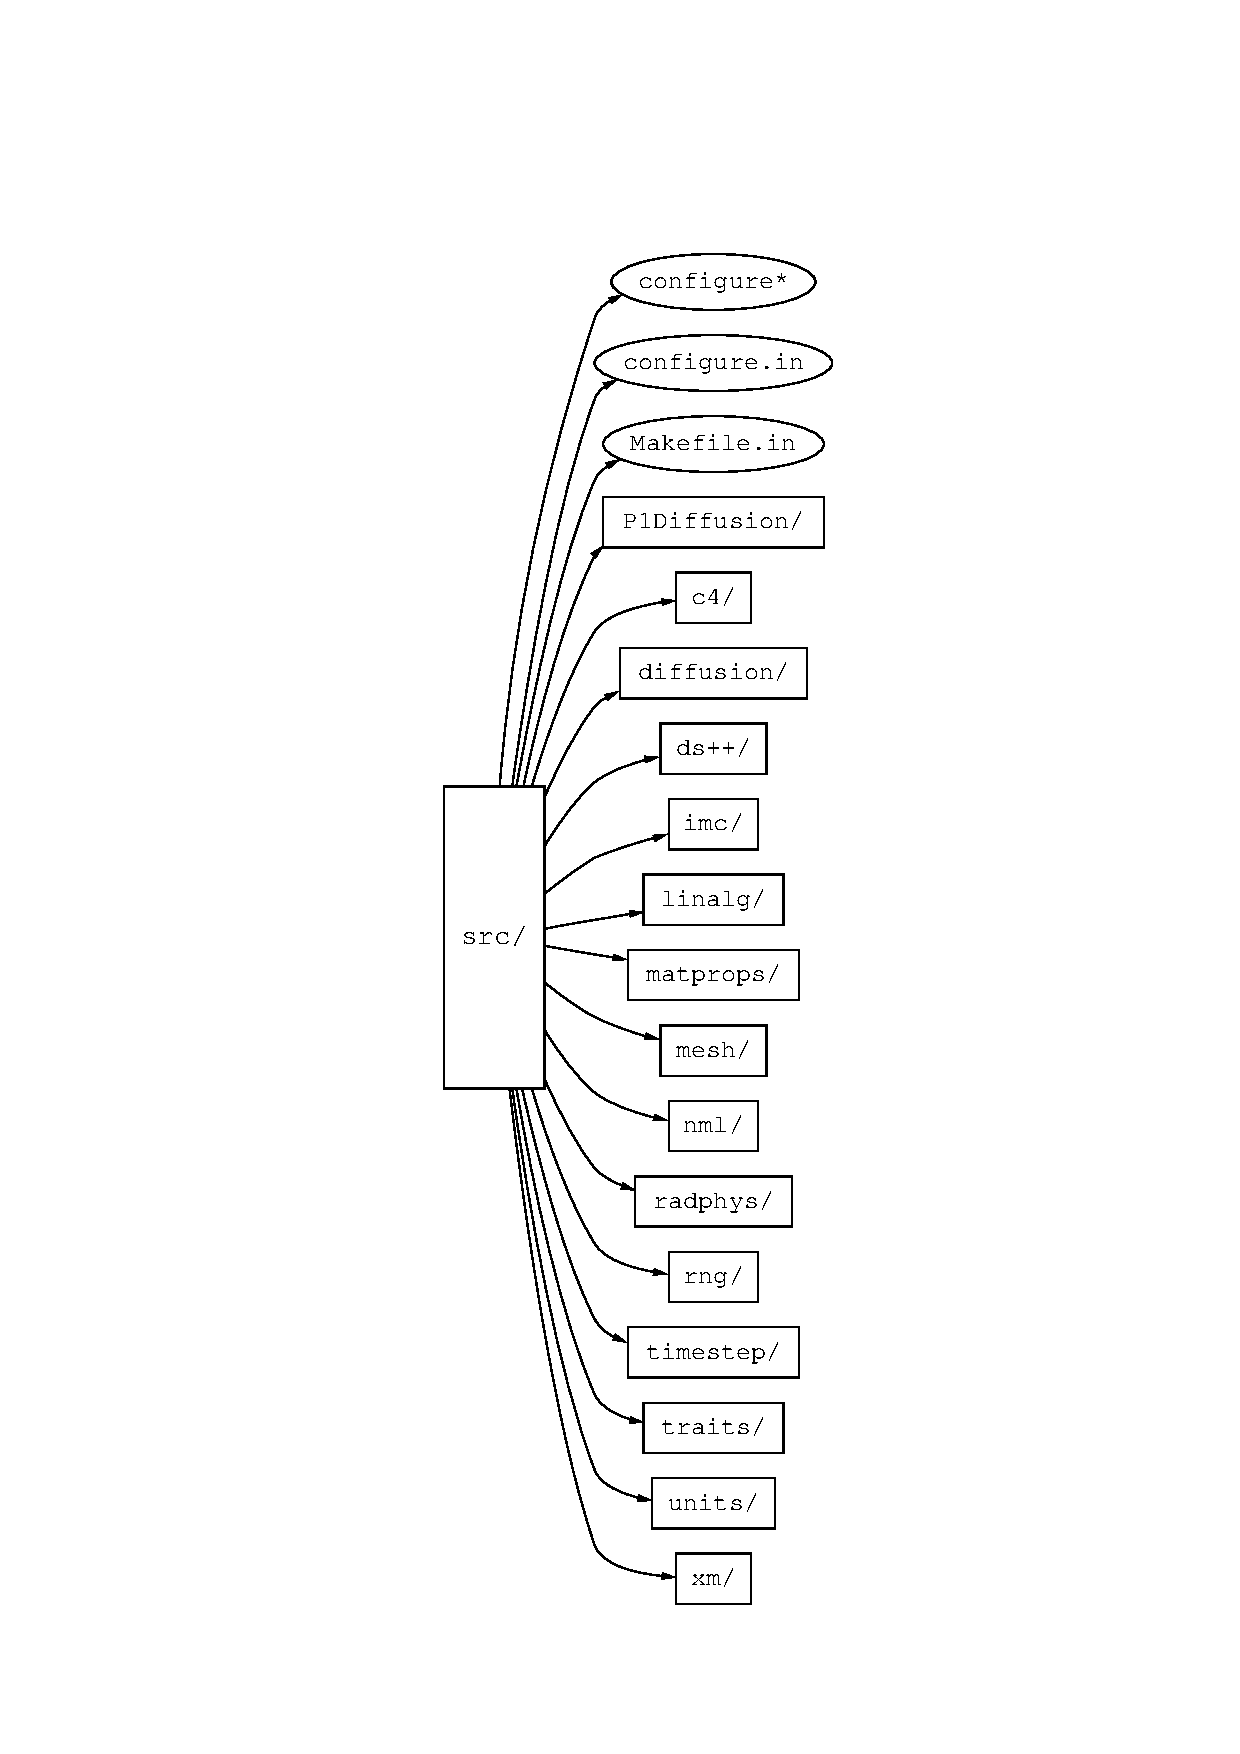
\includegraphics[clip,trim=12cm 2cm 5cm 0cm,width=1.3in]{fig/src_src}} & % trim=l b r t
      \subfloat[\comp{doc/}]{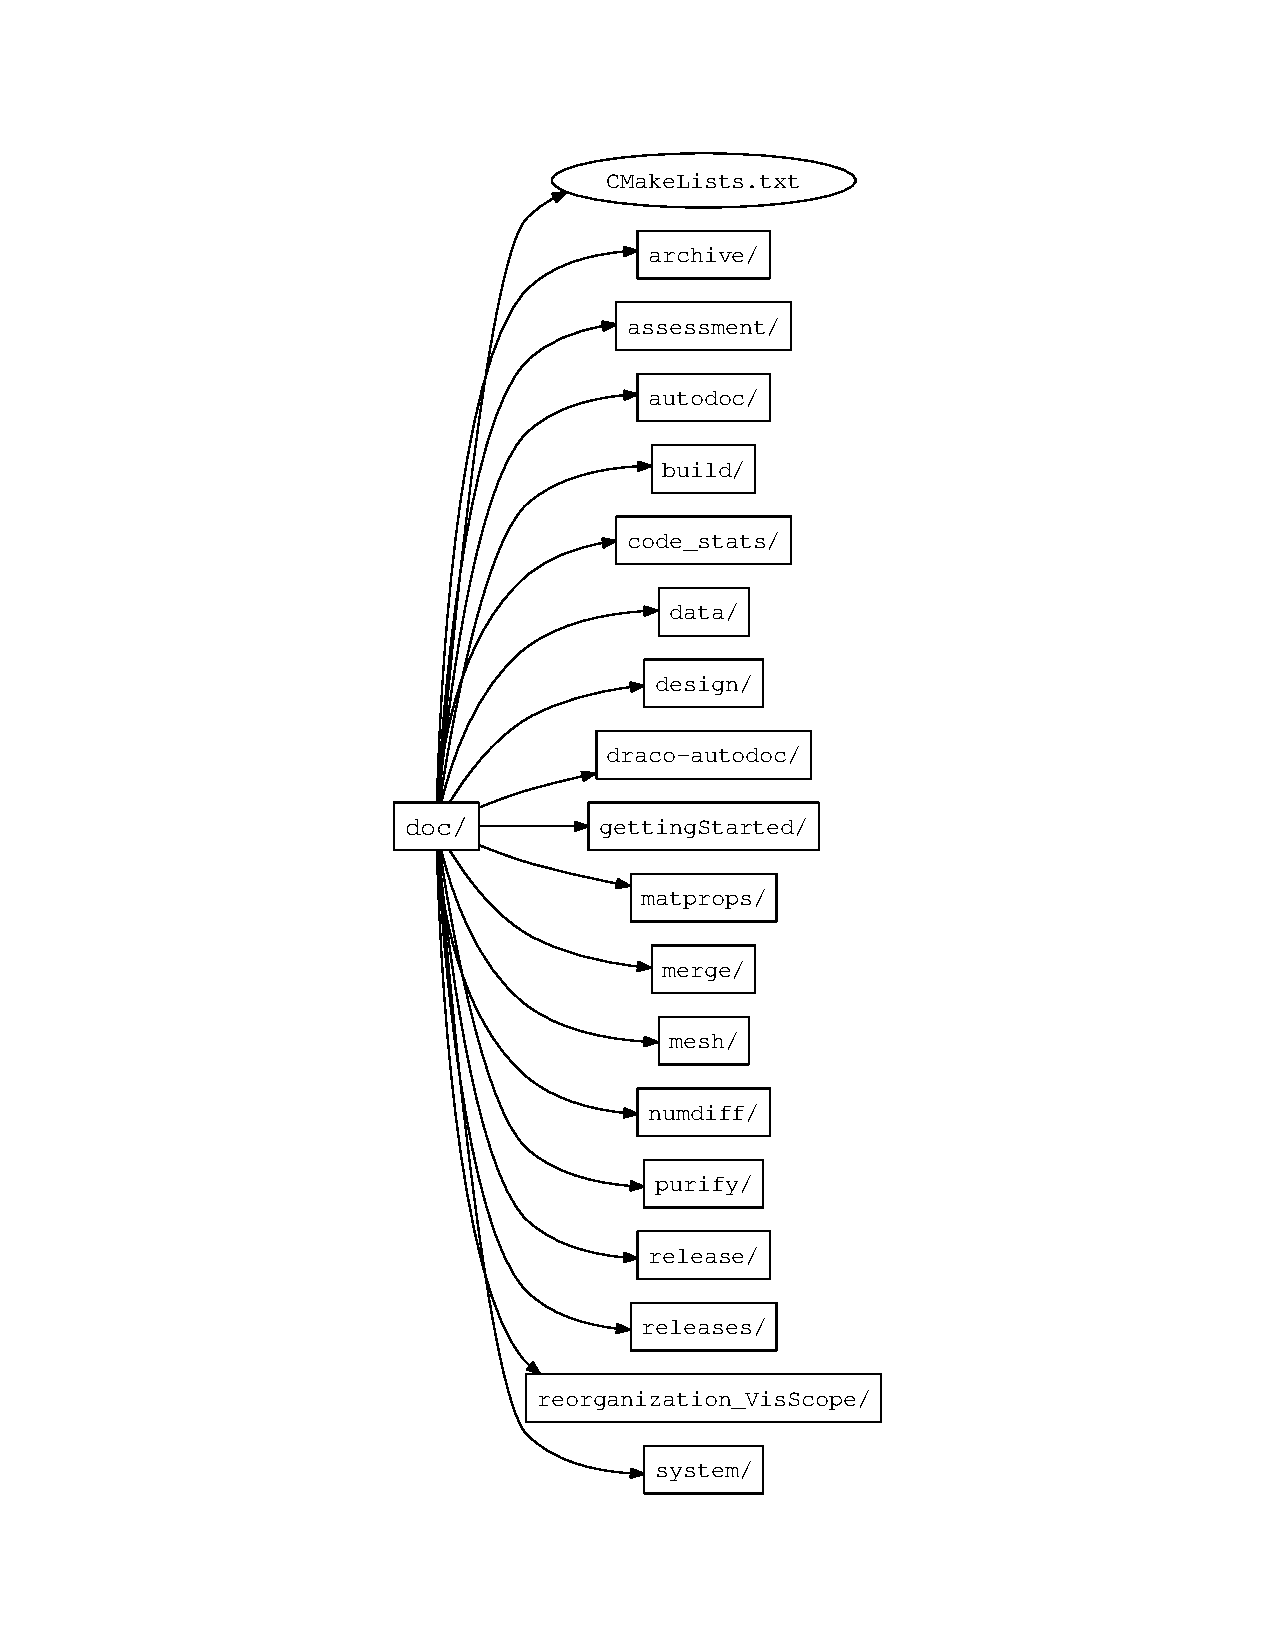
\includegraphics[clip,trim=9cm 1cm 8cm 0cm,width=1.0in]{fig/src_doc}} &
      \subfloat[\comp{config/}]{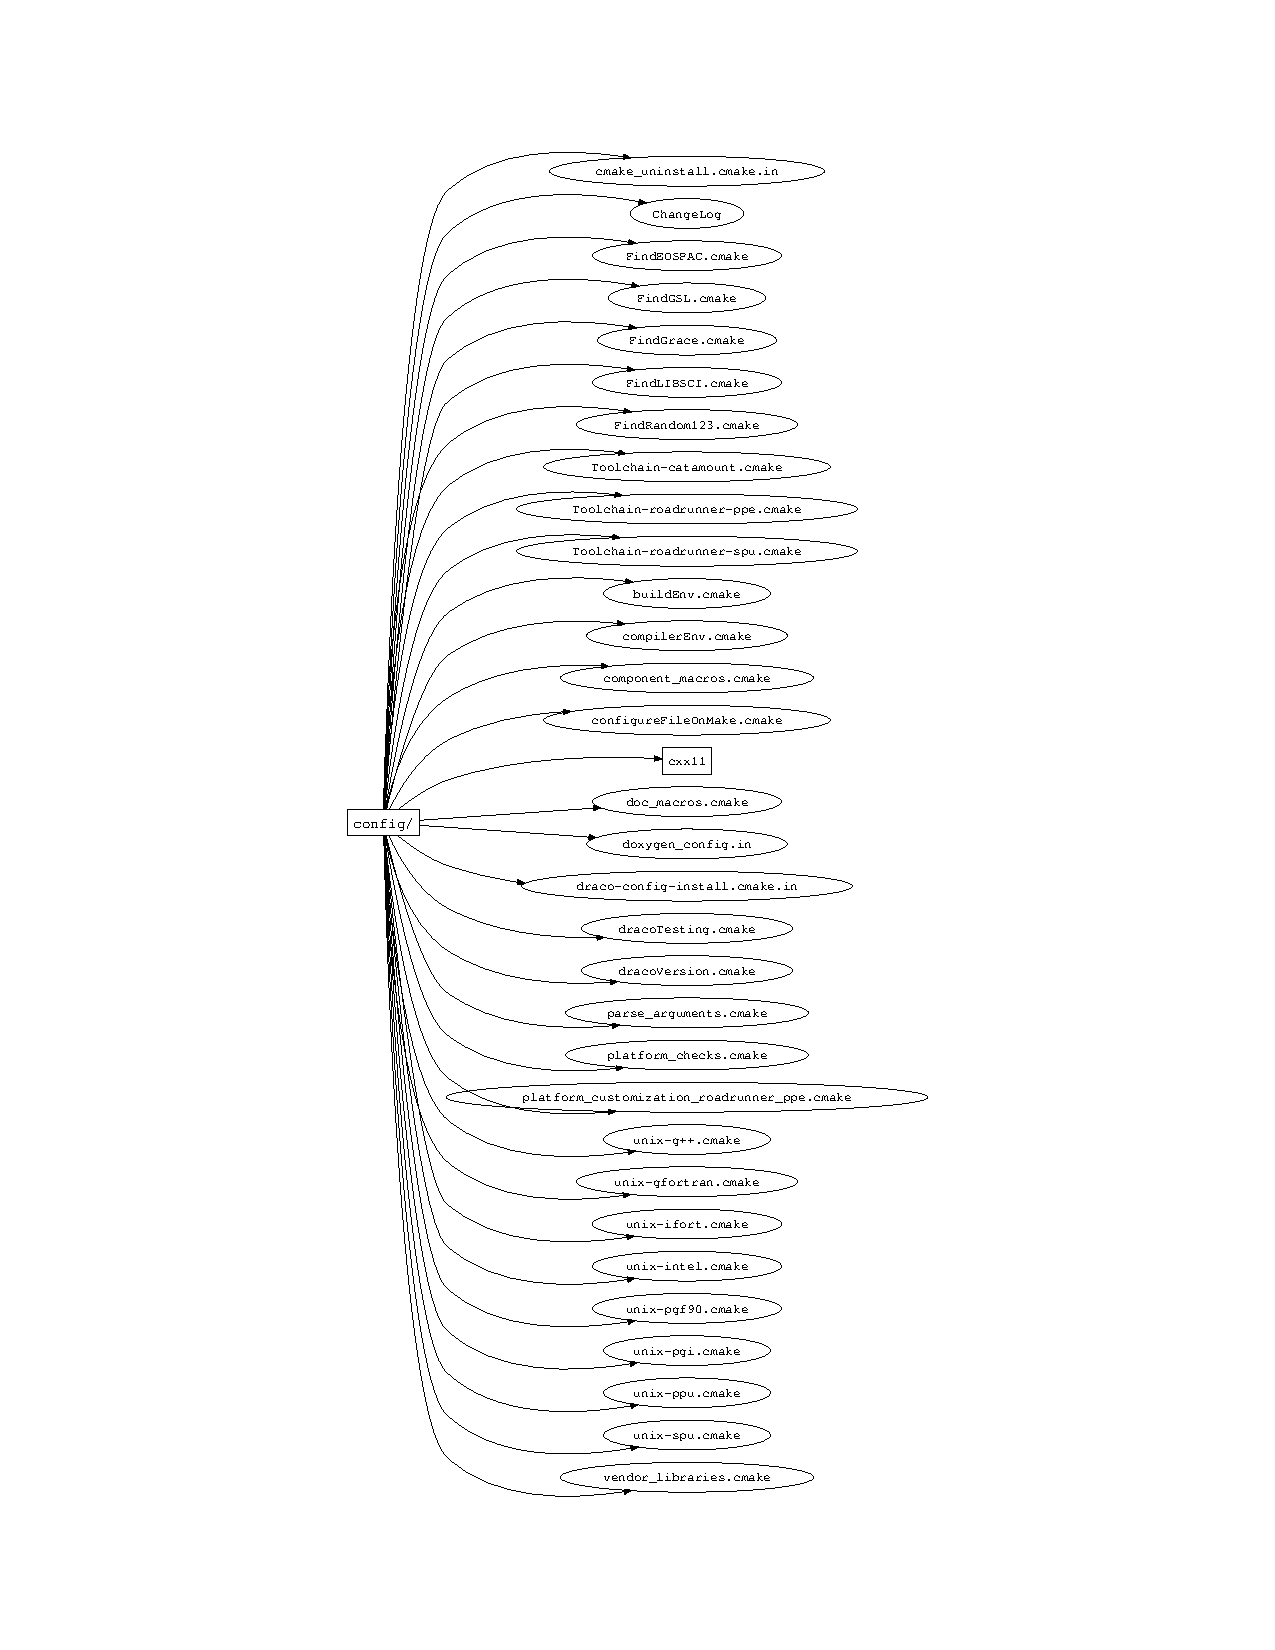
\includegraphics[clip,trim=4cm 2cm 10cm 0cm,width=2.0in]{fig/src_config}} 
      % \subfloat[\comp{tools/}]{\includegraphics[width=1.25in]{fig/src_tools.eps}} 
      \\
    \end{tabular}
  \end{center}
  \caption{Subdirectories under \comp{draco/}.  Directories are in
    boxes and files are in ellipses.}
  \label{fig:subdraco}
\end{figure}
complete source tree.
% not all directories under \comp{src/} will be released under certain \cvs\ checkouts.  
% The file \comp{draco\_config*} is a configure script that sets the proper paths to run configure in external directories.  
Under \draco\ there exists several files generated or needed by \cmake\ and \ctest.  The files \comp{CTestConfig.cmake} and \comp{CTestCustom.cmake} are read by \ctest\ and specify the location of the \draco\ dashboard and configuration setup for testing.  These settings include a list of source to omit from code coverage, tests to omit from dynamic analysis, warnings that should be ignored, etc.  The \comp{CMakeLists.txt} file is the primary build system configuration file parsed by \cmake\ in order to generate the build project (i.e.: Makefiles, project files, etc.).  The \comp{CMakeCache.txt} file is a template that developers can copy to their build sandbox and update initial build configuration settings before the first invocation of \cmake.  This file is not required by the \draco\ build system and is provided only as an aid for developers.
The \comp{*.cmake} files from the \comp{config} directory 
contains macro tests for configuring \draco.  Descriptions
of these files are given in Chap.~\ref{chap:extend}.  Finally, the
files \comp{Copyright}, \comp{ChangeLog}, and \comp{README.draco} are
descriptive ASCII files.

In the \comp{src/} directory there is a \comp{CMakeLists.txt} file that
instructs \cmake\ to setup the selected project generator, configure compiler options, run platform checks, locate and check vendor libraries, and tells \cmake\ to descend into each of the component directories for individual configuration. This file instructs \cmake\ to establish most of the build parameters and the master structure and inter-component dependencies.  The encapsulation and levelization of packages is controlled at this level.

In addition to the source code (\comp{.cc}, \comp{.hh}, and \comp{.h}
files), each component directory contains two build system files: 
A \comp{CMakeLists.txt} file controls the specific build instructions for the individual component including a list of sources to be compiled into a library.  The \comp{config.h.in} may not be provided with every component, but when it is provided it encapsulates preprocessor macro settings that are needed by the component.  Ref~\cite{autoconf} provides some background information on how the \comp{config.h.in} should be used.  Detailed discussions about how these files are used in \draco\ are given in Chaps.~\ref{chap:compile} and \ref{chap:adding}.

%In addition, each package directory may contain special files
%corresponding to the following formats
%\begin{verbatim}
%     <pkg>_<vendor>.h.in
%     Makefile.target
%     Makefile.srcs
%     Makefile.misc
%\end{verbatim}
%These files are used for special package configurations.  The file,
%\comp{<pkg>\_<vendor>.h.in}, is used to include vendor libraries that
%may not be installed in the standard \comp{\#include} and
%\comp{LD\_LIBRARY\_PATH} paths.  Details about the purpose of these
%files and their contents are given in Chaps.~\ref{chap:compile} and
%\ref{chap:adding}. 

Finally, each directory under \comp{src/} may contain source
subdirectories, \comp{doc/} subdirectories and \comp{autodoc} directories and should contain a \comp{test/} directory.  The
\comp{test/} directory holds component tests for the package.  Details
on how to compile the test directory using \ctest\ are given
in Chap.~\ref{chap:compile}.  Directions showing how to format
different test directories are given in Chap.~\ref{chap:adding}.

% ------------------------------------------ %
\subsection{Binary Directory Trees}

The \draco\ source is normally compiled in a separate, user-generated directory
tree called the \latin{target} or \latin{binary} directory tree\footnote{The GNU model normally uses the term \latin{target} directory while the \cmake\ community uses the term \latin{binary} directory, e.g.: \comp{PROJECT\_BINARY\_DIR}.}.  \index{binary directory} \index{target directory}  In this standard build mode, no files are
actually generated in the \draco\ source tree.  The \draco\ build system also supports building from within the source tree, but this mode of development is not recommended except in special circumstances (e.g: \soft{Eclipse} based projects work better when the source and binary tree are collocated). 

To configure \draco,
the user checks out a version of the source from \svn.  The checkout location is known as the \latin{source} directory.  In the \latin{binary} directory tree, the user runs \cmake\ with appropriate configure options.  These options can be provided (1) on the command line, (2) through the \cmake\ graphical interface via \comp{ccmake} \index{ccmake} or \comp{cmake-gui} \index{cmake-gui} or (3) by providing options in a \comp{CMakeCache.txt} \index{CMakeCache.txt} file located in the \latin{binary} directory.  \cmake\ will generate a directory tree
that is parallel to the \draco\ source tree with the appropriate
project and configuration files (e.g.: \comp{Makefile}, \comp{config.h}, \comp{draco.sln}, \comp{.project}, etc.).  Once the project files have been generated by \cmake, the compilation step can be initiated.  For a \latin{Unix Makefiles} based project this is accomplished by running \gmake\ from within the \latin{binary} directory.  The product of the compilation step is the generation of component libraries and executables by the selected compilers.  For non-\latin{Makefile} based projects, the \comp{all} or \comp{ALL\_BUILD} project target should be selected to begin compilation.

%In addition, \gmake\ installs the necessary \comp{.hh} and \comp{.h}
%files in a generated \comp{include/} directory.  Libraries are
%installed in a generated \comp{lib/} directory.  The \comp{include/}
%and \comp{lib/} directory locations are specified by the
%\comp{--prefix} tag in \autoconf.

For example, consider a parallel (MPI), debug configuration of \draco\ on a x86\_64 Linux
platform using the \soft{gcc} compiler suite.  The user might create a \latin{target} directory called
\comp{gcc\_mpid} and a \latin{build} directory under the target directory called \comp{draco}. After running \cmake\ with the
appropriate options\footnote{By default, the build system will configure for a debug build.  If MPI can be found on the local system, the build system will automatically enable parallel (MPI) features. The compiler set is chosen based on the value of environment variables \comp{CC}, \comp{CXX} and \comp{FC}.  If these variables are not set the build system will use whatever compiler it can find.  For this example, the configuration command is '\comp{cmake -DCMAKE\_INSTALL\_PREFIX=.. \$draco\_src\_dir}'},
%  and \gmake, 
the directory structure illustrated in Fig.~\ref{fig:build_tree} is generated.
\begin{figure}
  \centerline{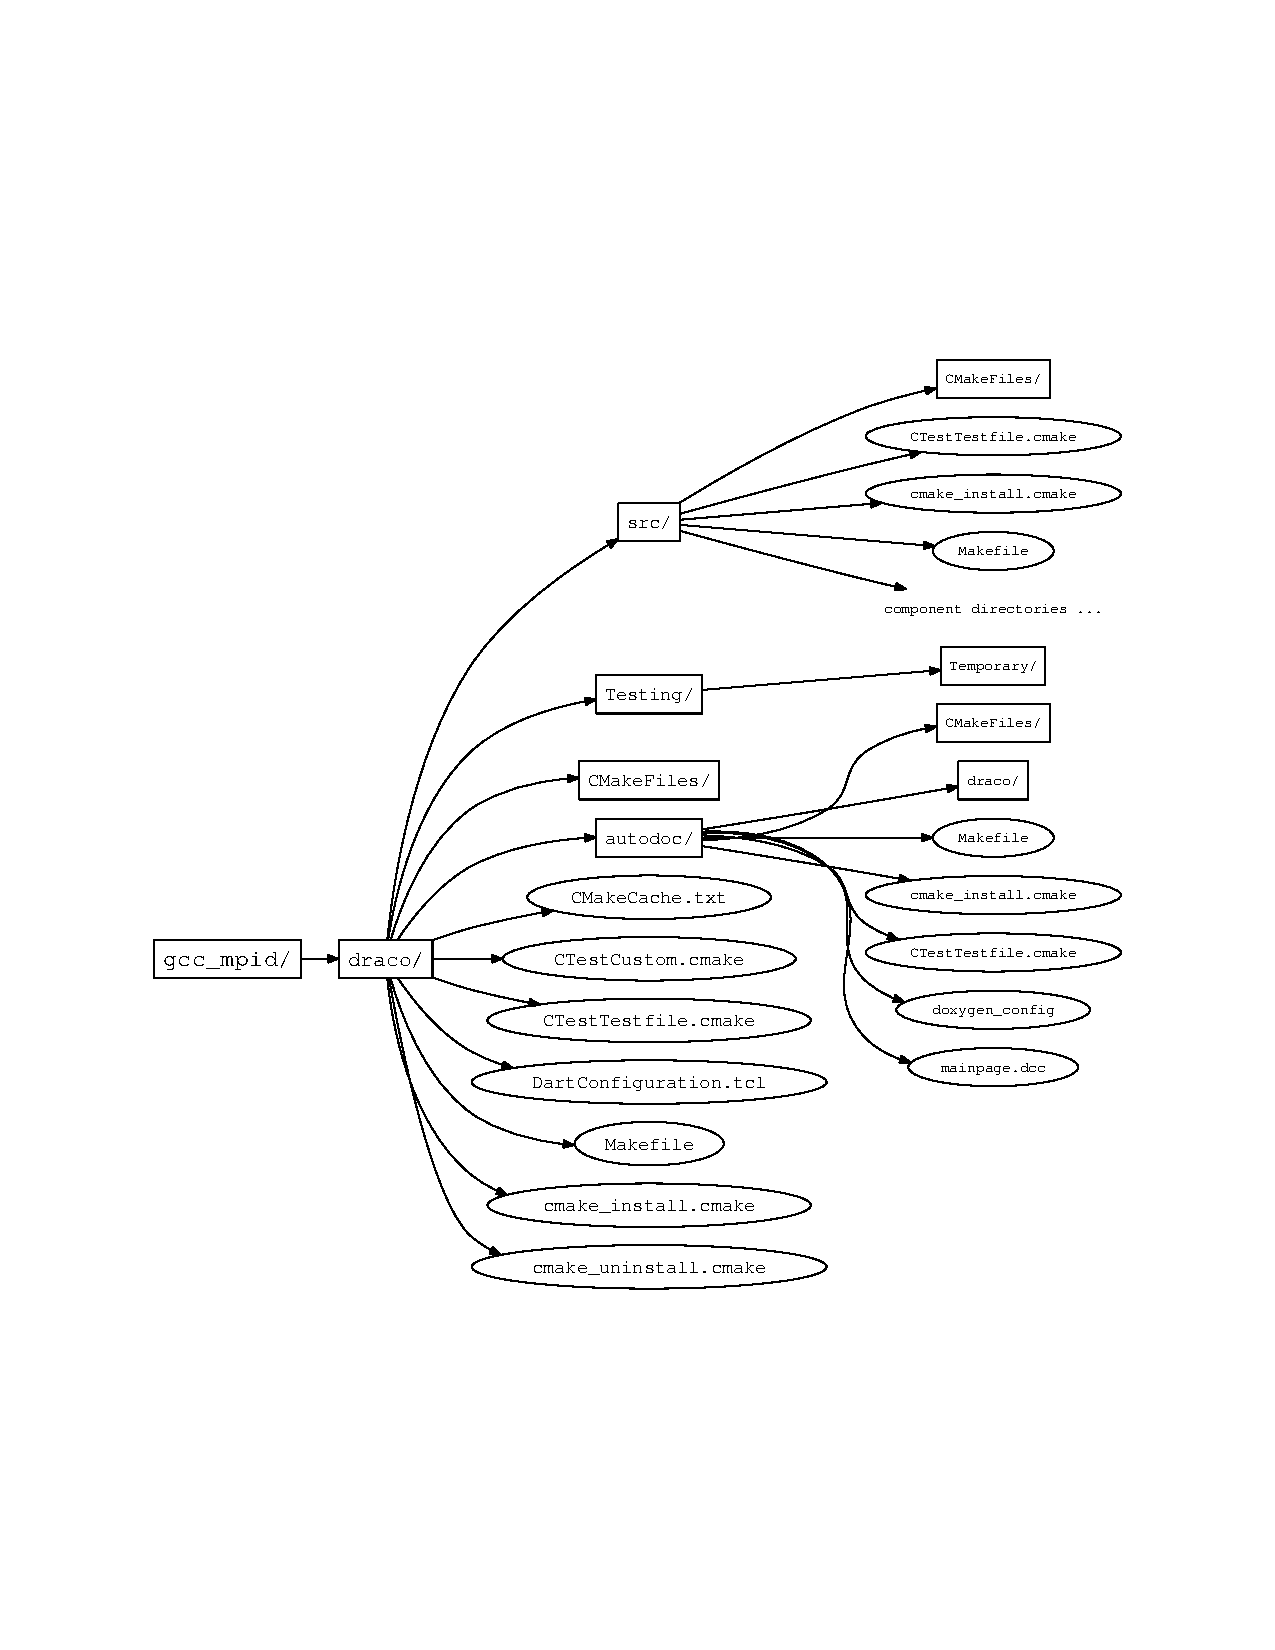
\includegraphics[width=6in]{fig/build_tree}}
  \caption{The \draco\ build tree after running \cmake\ for a Makefile-based project.  The \comp{source directories} are shown in
    Fig.~\ref{fig:subdraco}a. The \comp{doc directories} are shown in
    Fig.~\ref{fig:subdraco}b.}  The binary tree for \sys{Eclipse CDT4 - Unix Makefile} based projects will match this layout but will also include two additional dot files: \comp{.cproject} and \comp{.project}.
  \label{fig:build_tree}
\end{figure}
Inside of each component directory are Makefiles and configuration files
generated by \cmake.  Object (\comp{.o}) files are stored in the \comp{CMakeFiles/} directory along with specialized build and dependency instructions (\comp{depend.make}, \comp{flags.make}, \comp{link.txt}, etc.)
% Also, after building, the automatic
%dependency files (\comp{.cc.d} and \comp{.c.d}) will be found here
%along with the object (\comp{.o}) files.  

After building the project (possibly by running \make), the generated libraries and binary files will show up in the component directories.  The \draco\ build system is able to execute the compile step in parallel, utilizing all of the available local cores.  For \sys{Unix Makefile} based project, the option \comp{-j N} should be given to \make\ where the value of N is set to be the number of available cores on the local machine\footnote{Some developers have reported good results when requesting ~50\% more jobs than cores.  For example, for a machine that has 8 cores, the command \comp{make -j 12} has worked well.}.  \index{parallel make}

The generated files can be installed to the \latin{target} directory by building the \comp{install} target.  For development, it is a common practice to set the \latin{install} location to be the platform \latin{target} directory. \index{target directory} \index{install directory} This allows the generated libraries, headers and executable files to be stored under an appropriately named directory like \comp{gcc\_mpid} or \comp{intel10\_openmpi145\_rwdi} (Version 10 Intel compilers, OpenMPI version 1.4.5 and ReleaseWithDebInfo build model).  Running the \comp{install} target will add the \comp{lib/}, \comp{bin/}, \comp{include/} and \comp{config} directories under the  \latin{target} directory as shown in Figure~\ref{fig:build_tree_post_install}.
\begin{figure}
  \centerline{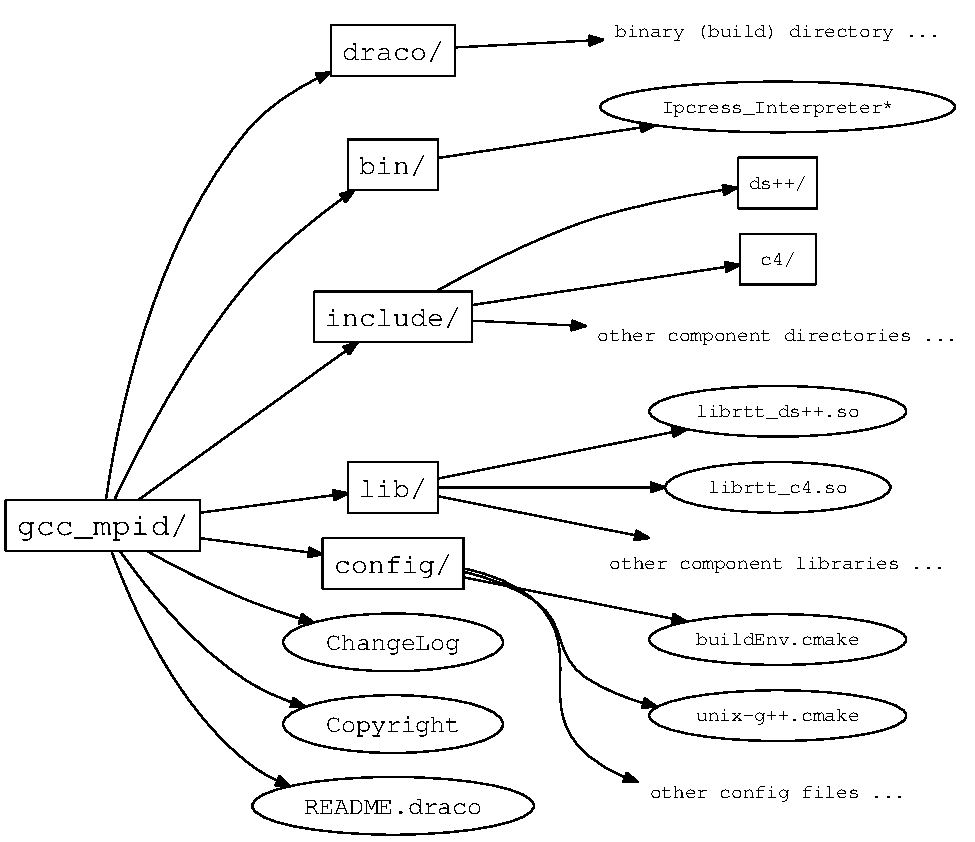
\includegraphics[width=6in]{fig/build_tree_post_install}}
  \caption{The \draco\ build tree after running \comp{make install} for a Makefile-based project.  The \latin{install} target creates  the \comp{lib/}, \comp{bin/}, \comp{include/} and \comp{config} directories under the  \latin{target} directory.  The target directory is specified at \latin{configure} time by setting the \cmake\ variable \comp{CMAKE\_INSTALL\_PREFIX}.}
  \label{fig:build_tree_post_install}
\end{figure}

%Appropriately, any files
%needed by a client system are found in the \comp{include/} and
%\comp{lib/} directories.  Also, multiple builds with different
%configuration options may be performed simultaneously.  All one has to
%do is generate a build directory for each configure.  

In many cases, \draco\ based software projects will be configured and compiled alongside \draco.  In this case, a binary directory for the client (e.g.: \clubimc\ or \capsaicin) might be found parallel to the \comp{draco} binary directory (see Fig.~\ref{fig:build_tree_post_install}) and the the client products (headers, libraries, etc.) are installed into the same target directory used by \draco.  Details on how to configure and compile \draco\ are found in Chap.~\ref{chap:compile}, \S~\ref{sec:configuring_draco} and \S~\ref{sec:building_draco}.


%%---------------------------------------------------------------------------%%

\section{Coding Conventions}
\label{sec:codeconventions}

\draco\ does not adhere strictly to any code convention for formatting, but it is recommended that developers attempt to follow the styles already used in existing source code.  The following subsections list specific code conventions that are required by \draco.

\subsection{File Extensions}
\label{sec:cc-fileext}

Table~\ref{tab:fileext} lists file extension standards used by \draco\ along with a description of the expected content type.
%
\begin{table}
  \begin{center}
    \caption{Draco Coding Conventions: Standard File Extensions}
    \label{tab:fileext}
    \begin{tabular}{p{0.5in}p{2.0in}p{3.5in}}\hline\hline
    
    File Extension & Description & Details \\ \hline
    \comp{.h} & ANSI C header file & Rarely used in \draco\ except for wrapping calls to vendor functions. \\
    \comp{.c} & ANSI C implementation file & Rarely used in \draco\ except for wrapping calls to vendor functions. \\
    \comp{.hh} & C++ declarations file & Common file that provide class and function declarations, including templated functions and classes.\\  
    \comp{.i.hh} & C++ inline implementation file & C++ implementation instructions that could be placed directly in the \comp{.hh} file.  These implementations are for inlined functions or implicitly instantiated template functions.  This file is always included directly by the \comp{.hh} file after all declarations have been made. \\
    \comp{.t.hh} & C++ template implementation file & C++ implementation instructions for explicitly instantiated functions.  This file always includes the associated \comp{.hh} file and is only included by an explicit instantiation file(\comp{\_pt.cc}). \\
    \comp{.cc} & C++ implementation file & C++ implementation instructions for functions declared in the \comp{.hh} file that are not to be inlined and are not template functions. \\
    \comp{\_pt.cc} & C++ explicit instantiation file & C++ explicit instantiations of templated classes and functions found in the associated declarations file. \\
    \comp{.in} & Files that must be processed & Usually found as \comp{config.h.in} that is processed into \comp{config.h} and provides preprocessor definitions used by the local component. \\
    \comp{.cmake} & \cmake\ build system file & Additional build system commands that have been extracted form \comp{CMakeLists.txt} files to improve reuse via cmake-macros. \\
	\hline \hline

    \end{tabular}
  \end{center}
\end{table}


\subsection{Tabs and editor width}
\label{sec:cc-tabs}

\draco\ developers have found that code is most cleanly viewed on various editors if spaces are used in place of tabs and the maximum column width is restricted to 80 columns.

%%---------------------------------------------------------------------------%%

\section{Summary}

In this chapter we have summarized the basic structure of the \draco\ 
build system.  We have illustrated the requirements for the \draco\ 
build system.  In the following chapters we will elaborate on the
details of how to configure, build, and test \draco\ installations.


%%---------------------------------------------------------------------------%%
%% compile.tex
%% Time-stamp: <99/02/11 18:42:51 tme>
%% explains how to configure and compile the draco library
%%---------------------------------------------------------------------------%%

\chapter{Configuring and Compiling Draco}
\label{chap:compile}

This chapter describes how to configure and build \draco.  All
configure\index{configure} options will be illuminated in detail.  After reading this
chapter the user and/or developer will know how to build \draco\ on
multiple platforms, for various build project systems (\soft{Makefiles}, \soft{Eclipse}, \soft{XCode}, etc.) and for different options.  In addition, the user
will know how to build multiple versions of \draco\ simultaneously.
To illucidate the concepts about \draco\ dependencies, configuration
options, and build targets, \S~\ref{sec:examples} provides several
examples that show how to build \draco\ for various configurations.

%%---------------------------------------------------------------------------%%

\section{Draco Dependencies}
\label{sec:draco_dependencies}

As mentioned in \S~\ref{sec:overview_of_draco}, \draco\ is based on
the concept of levelized design~\cite{la96} \index{levelized design}.  A component-level diagram
is shown in Fig.~\ref{fig:level}\index{levelized design}.  By following the dependency lines
\begin{figure}
  \centerline{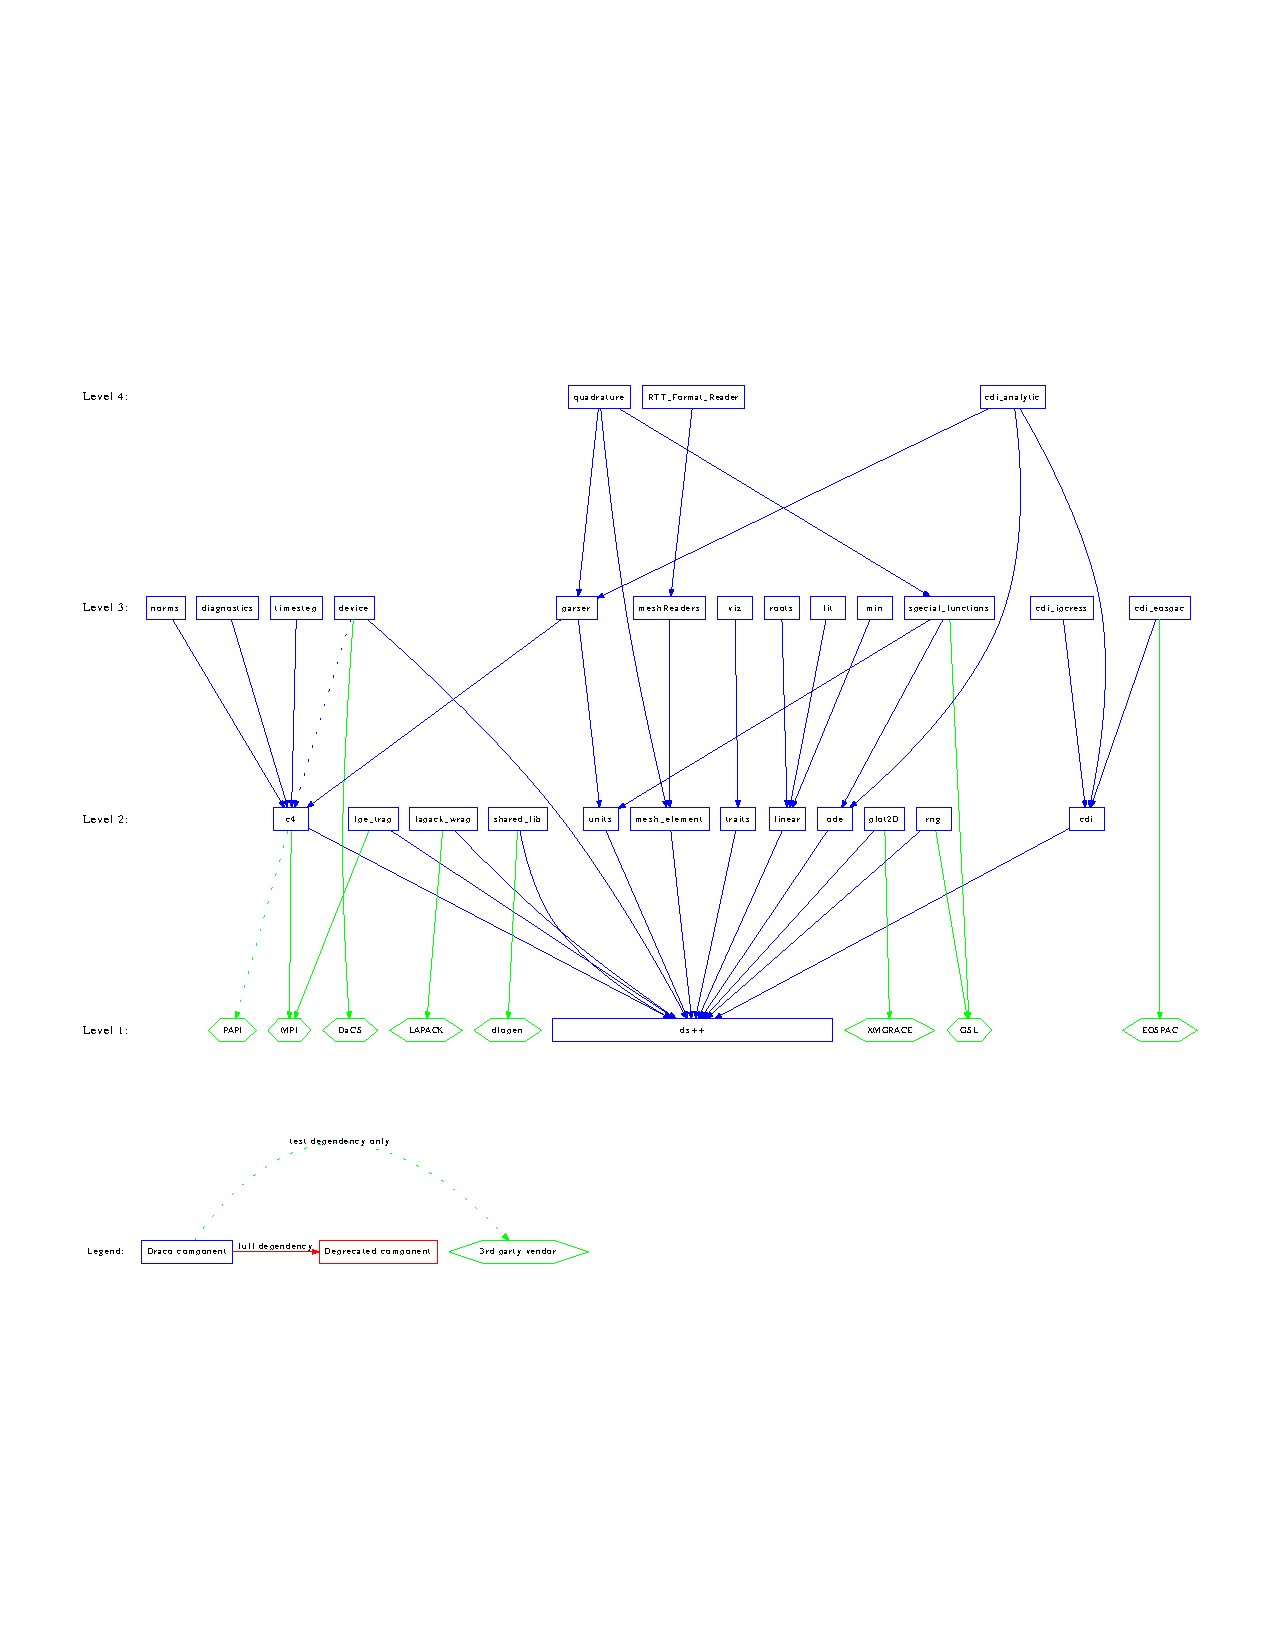
\includegraphics[angle=90]{fig/level}}
  \caption{Component-level diagram for \draco.}
  \label{fig:level}
\end{figure}
of this diagram, one can determine the exact dependencies required by
each component in \draco.  Thus, to compile a component static library, all of
the dependencies, both explicit and implicit, must be included when linking.

In addition to the direct component dependencies illustrated in
Fig.~\ref{fig:level}, the \comp{\vble{pkg}/test/} directory may
require additional components for its compartmentalized unit tests.  For example,
\comp{device} does not explicitly require \comp{c4}, but \comp{c4} and \comp{MPI} are required for compiling the unit tests for \comp{device}.  Unit test dependencies are included in this component-level diagram and dependencies unique to the tests are represented by dotted lines.   
%Figure~\ref{fig:test_level} shows the \draco\ package
%dependency tree
%\begin{figure}
%  \centerline{\includegraphics{fig/test_level.eps}}
%  \caption{Package-level diagram for \draco.  Test dependencies are
%    noted by the dotted arrows.}
%  \label{fig:test_level}
%\end{figure}
%with package test dependencies included.
The policy in \draco\ is that
test directories are responsible for their own template instantiations\index{policy!templates} in \comp{*\_pt.cc} files.
Directions showing how to include test directory dependencies are given in Chap~\ref{chap:adding}. 

When using \draco\ on an external product, all component dependent
libraries must be included.\index{dependencies!component}  The list of necessary libraries for
linking a package is given in Table~\ref{tab:depends}.  In summary,
\begin{table}
  \caption{
    Listing of \draco\ component dependencies.  The \draco\ component
    dependencies are the sum of the explicit and implicit dependencies.
    For general package use, only components listed under \draco\ Component
    Dependencies (Explicit and Implicit) are required.  The components
    listed under \draco\ Component Test Dependencies are only required for
    testing.}
  \label{tab:depends}
  \begin{center}
    \begin{tabular}{lclll} \hline\hline
      \multicolumn{1}{c}{\draco\ Package} & Level &
      \multicolumn{1}{c}{\draco\ Explicit} &
      \multicolumn{1}{c}{\draco\ Implicit} &
      \multicolumn{1}{c}{\draco\ Package} \\ 
      & & \multicolumn{1}{c}{Package Dependencies} &
      \multicolumn{1}{c}{Package Dependencies} &
      \multicolumn{1}{c}{Test Dependencies} \\ \hline
       \dsxx & 1 & - & - & - \\

%       \xm & 1 & - & - & - \\
%       \pkg{nml} & 2 & \dsxx & - & - \\
       \cfour & 2 & \dsxx & - & - \\
       \pkg{cdi} & 2 & \dsxx & - & - \\
       \pkg{fpe\_trap} & 2 & \dsxx & - & - \\
       \pkg{lapack\_wrap} & 2 & \dsxx & - & - \\
       \pkg{linear} & 2 & \dsxx & - & - \\
       \pkg{mesh\_element} & 2 & \dsxx & - & - \\
       \pkg{ode} & 2 & \dsxx & - & - \\
       \pkg{plot2D} & 2 & \dsxx & - & - \\
       \rng & 2 & \dsxx & - & - \\  
       \pkg{shared\_lib} & 2 & \dsxx & - & - \\
       \pkg{traits} & 2 & \dsxx & - & -  \\ 
       \pkg{units} & 2 & \dsxx & - & - \\       
       
%       \pkg{diffusion} & 3 & \pkg{nml} & \dsxx & \pkg{mesh} \\
%         \imc & 3 & \dsxx, \rng, \cfour & - & - \\
%       \pkg{linalg} & 3 & \dsxx, \cfour, \pkg{nml} & - & - \\
%       \pkg{mesh} & 3 & \dsxx, \pkg{xm}, \pkg{traits}, \cfour,
%       \pkg{nml} & - & - \\
%       \pkg{radphys} & 3 & \pkg{traits}, \pkg{units} & - &
%       \pkg{mesh} \\ 
       \pkg{cdi\_ipcress} & 3 & \pkg{cdi} & \dsxx & - \\
       \pkg{cdi\_eospac} & 3 & \pkg{cdi} & \dsxx & - \\
       \pkg{device} & 3 & \dsxx & - & \cfour \\
       \pkg{diagnostics} & 3 & \cfour & \dsxx & - \\
       \pkg{fit} & 3 & \pkg{linear} & \dsxx & - \\
       \pkg{meshReaders} & 3 & \pkg{mesh\_element} & \dsxx & - \\
       \pkg{min} & 3 & \pkg{linear} & \dsxx & - \\
       \pkg{norms} & 3 & \cfour & \dsxx & - \\
       \pkg{parser} & 3 & \cfour, \pkg{units} & \dsxx & - \\
       \pkg{roots} & 3 & \pkg{linear} & \dsxx & - \\
       \pkg{special\_functions} & 3 & \pkg{ode}, \pkg{units} & \dsxx & - \\
       \pkg{timestep} & 3 & \cfour & \dsxx & - \\
       \pkg{viz} & 3 & \pkg{traits} & \dsxx & - \\
       
       \pkg{cdi\_analytic} & 4 & \pkg{parser}, \pkg{ode}, \pkg{cdi} & \cfour, \dsxx, \pkg{units} & - \\
       \pkg{quadrature} & 4 & \pkg{parser},  & \cfour, \dsxx, \pkg{units},  & - \\
        &  & \pkg{mesh\_element},  & \pkg{ode} &  \\
        &  & \pkg{special\_functions} &  &  \\
              
%       \pkg{matprops} & 4 & \dsxx, \pkg{traits}, \pkg{units},
%       \pkg{radphys} & - & \pkg{mesh} \\
%       \pone & 4 & \dsxx, \pkg{linalg}, \pkg{diffusion} & \cfour,
%       \pkg{nml} & \pkg{mesh} \\ 
\hline\hline
    \end{tabular}
  \end{center}
\end{table}
when a \draco\ component is used in an external code, all libraries
listed under \draco\ Package Dependencies (Explicit and Implicit) in
Table~\ref{tab:depends} must be included on the link line.  The
packages listed under \draco\ Package Test Dependencies do not have to
be linked.  We note that \draco\ packages know both their package
dependencies and their package test
dependencies (Fig.~\ref{fig:level}).  The external \draco\ client
must be aware that when using a \draco\ package all of the packages
dependencies (not package test dependencies) must be included.

Some components in \draco\ require external vendor support.\index{dependencies!vendor}
Additionally, some configuration options in \draco\ require external
vendor support.  Table~\ref{tab:vendor} lists all of the present
\begin{table}
  \caption{Vendors required by packages in \draco.  Implicit are the
    \cpp\ Standard Template Library (STL), the \cc\ Standard
    Library, and compiler libraries (\comp{libF77}).  Systems
    libraries  (\comp{sys/time.h}) are also not included.}
  \label{tab:vendor}
  \begin{center}
    \begin{tabular}{lclc}\hline\hline
      \multicolumn{1}{c}{Package} & Level & \multicolumn{1}{c}{Vendor Options}
      & Required \\ \hline
      \dsxx & 1 & - &  - \\
      
%      \xm & 1 & - & - \\
      \cfour & 2 & \mpi, \sys{OpenMP} & no \\
      & & \sys{PAPI} & no \\
      \pkg{cdi} & 2 & - & - \\
      \pkg{fpe\_trap} & 2 & \mpi & no \\
      \pkg{lapack\_wrap} & 2 & \sys{LAPACK}, \sys{BLAS} & yes \\
      \pkg{linear} & 2 & - & - \\
      \pkg{mesh\_element} & 2 & - & - \\
      \pkg{ode} & 2 & - & - \\
      \pkg{plot2D} & 2 & \sys{XM Grace} & yes \\
      \pkg{rng} & 2 & \sys{GSL} & yes \\
      \pkg{shared\_lib} & 2 & \sys{dlopen} & yes \\
      \pkg{traits} & 2 & - & - \\
      \pkg{units} & 2 & - & - \\
      
%      \pkg{nml} & 2 & - & - \\
%      \rng & 2 & \sprng & yes  \\
%      \pkg{units} & 2 & - & - \\
%      \pkg{diffusion} & 3 & - & - \\
%      \imc & 3 & - & -  \\
%      \pkg{linalg} & 3 & \pcglib & yes \\
%      \pkg{mesh} & 3 & - & - \\
    %  \pkg{radphys} & 3 & - & - \\ 
          \pkg{cdi\_eospac} & 3 & \sys{EOSPAC} & yes \\
      \pkg{cdi\_ipcress} & 3 & - & - \\
      \pkg{device} & 3 & \sys{DaCS} or \sys{CUDA} & yes \\
       &  & \sys{MPI} & no \\
      \pkg{diagnostics} & 3 & \sys{MPI} & no \\
      \pkg{fit} & 3 & - & - \\
      \pkg{meshReaders} & 3 & - & - \\
      \pkg{min} & 3 & - & - \\
      \pkg{norms} & 3 & \sys{MPI} & no \\
      \pkg{parser} & 3 & \sys{MPI} & no \\
      \pkg{roots} & 3 & - & - \\
      \pkg{special\_functions} & 3 & \sys{GSL} & yes \\      
      \pkg{timestep} & 3 & \sys{MPI} & no \\
      \pkg{viz} & 3 & - & - \\
       
%      \pkg{matprops} & 4 & - & - \\
%      \pone & 4 & - & - \\ 
      \pkg{cdi\_analytic} & 4 & \sys{MPI} & no \\
      \pkg{quadrature} & 4 & \sys{GSL} & yes \\
       &  & \sys{MPI} & no \\
      \pkg{RTT\_Format\_Reader} & 4 & - & - \\

\hline\hline
    \end{tabular}
  \end{center}
\end{table}
components in \draco\ and the vendors that are required to build those
components.  Also, because \draco\ is based on the concepts of levelized
design as stated above, each component in \draco\ may have dependencies
on lower level \draco\ components.  In these cases only the dependencies
of the specified package are of interest.  For example, the \pkg{parser} 
component itself requires no external vendors; however, \pkg{parser} requires
\cfour\ that does require an external vendors (\sys{MPI}).  The build system
knows the \draco\ dependencies of each component; however, the external
user (client) must be aware of vendor requirements in the component
dependencies.  If a required vendor library is not found by the \draco\ build system, that component will be omitted from the configuration.  For example, if \sys{LAPACK} is not found on the current machine, the \draco\ build system will not attempt to configure or compile \pkg{lapack\_wrap}.  Some dependencies, like \sys{PAPI} are only used for profiling and if activated anywhere, must be activated everywhere.
Tables~\ref{tab:depends} and \ref{tab:vendor} can be
used to determine what \draco\ components and what vendor libraries must
be included when linking to a specific \draco\ components.  Details on
how to configure components with certain vendor options are given in
\S~\ref{sec:configuration_options}.  Information on linking to
specific libraries is given in Appendix~\ref{app:vendor_libs}.

To summarize the preceding we will employ a simple example.  Let us
assume that a user wishes to use the \pkg{quadrature} package.  Additionally,
this configuration will be a parallel configuration using
\mpi\,\footnote{\cfour\ is \draco's communication package and
  determines if the resulting code will be scalar or parallel.}.  From
Table~\ref{tab:depends} we see that \pkg{quadrature} is dependent on the \draco\ 
packages \pkg{special\_functions}, \pkg{parser}, \pkg{mesh\_element}, \pkg{ode}, \dsxx, \pkg{units}, and \cfour.  From Table~\ref{tab:vendor} we see
that \pkg{ode} requires the \sys{GSL} library and \cfour\ requires the \mpi\ 
library.  Accordingly, for a \sys{UNIX} \sys{Makefile}-based build, the following libraries must be included on the
link line:
\begin{verbatim}
     -lrtt_quadrature -lrtt_parser -lrtt_special_functions -lrtt_c4 -lrtt_units \
     -lrtt_mesh_element -lrtt_ode -lrtt_ds++ \
     -lgsl -lgslcblas \
     -lmpi_cxx -lmpi -lopen-rte -lopen-pal
\end{verbatim}
where \comp{-lgsl -lgslcblas} are the \pkg{GSL} libraries (see \S~\ref{appsec:gsl}) and \comp{-lmpi\_cxx -lmpi -lopen-rte -lopen-pal} are the \mpi\ libraries (see \S~\ref{appsec:mpi}).  Additional system libraries may also be required (e.g.: \comp{-ldl -lnsl -lutil -lm}).
This example assumes that all of the following library locations are
defined in \ldlib.  Thus, even though \pkg{quadrature} does not explicitly depend
on \mpi\ or \sys{GSL}, it uses \draco\ packages (\cfour\ and \pkg{special\_functions}) that
do require these libraries.  In practice, the \draco\ build system attempts to find and use full paths to vendor and \draco\ component libraries so that \ldlib\ does not need to be manipulated by the developer or software user.  The build system also locates and sets all of the libraries required or each vendor so that a \draco\ component or client only needs to specify that it should link to a set of libraries provided by the \cmake\ variable  \$\vble{\{\$\{VENDOR\}}\comp{\_LIBRARIES\}}.

%%---------------------------------------------------------------------------%%

\section{Draco Package Products}

In Chap.~\ref{chap:model} we insinuated that each \draco\ component
provides a library.  For example, \pkg{quadrature} provides
\comp{librtt\_quadrature.a(.so)} on \sys{UNIX} systems.  This is not entirely accurate.  Some \draco\
packages, \pkg{traits} is an example, consist only of header files and do not
provide a compiled library.  Users need to be aware of this fact when
linking \draco\ components.  If a \draco\ client uses the \pkg{viz}
package, which requires \pkg{traits}, linking \comp{-lrtt\_traits} is incorrect because
\pkg{traits} does not produce a library.  Table~\ref{tab:products} lists the
\begin{table}
  \caption{Products for \draco\ packages.}
  \label{tab:products}
  \begin{center}
    \begin{tabular}{lccc}\hline\hline
      \multicolumn{1}{c}{Package} & \comp{include/} & \comp{lib/} &
      \comp{bin/} \\ \hline
      
      \dsxx & yes & yes &  no \\
      
      \cfour & yes & yes & no \\
      \pkg{cdi} & yes & yes & no \\
      \pkg{fpe\_trap} & yes & yes & no \\
      \pkg{lapack\_wrap} & yes & no & no \\
      \pkg{linear} & yes & yes & no \\
      \pkg{mesh\_element} & yes & yes & no \\
      \pkg{ode} & yes & yes & no \\
      \pkg{plot2D} & yes & yes & no \\
      \pkg{rng} & yes & yes & no \\
      \pkg{shared\_lib} & yes & yes & no \\
      \pkg{traits} & yes & no & no \\
      \pkg{units} & yes & yes & no \\
      
      
      
      \pkg{cdi\_eospac} & yes & yes & no \\
      \pkg{cdi\_ipcress} & yes & yes & yes \\
      \pkg{device} & yes & yes & no \\
      \pkg{diagnostics} & yes & yes & no \\
      \pkg{fit} & yes & yes & no \\
      \pkg{meshReaders} & yes & yes & no \\
      \pkg{min} & yes & yes & no \\
      \pkg{norms} & yes & yes & no \\
      \pkg{parser} & yes & yes & no \\
      \pkg{roots} & yes & yes & no \\
      \pkg{special\_functions} & yes & yes & no \\
      \pkg{timestep} & yes & yes & no \\
      \pkg{viz} & yes & yes & no \\
                 
      \pkg{cdi\_analytic} & yes & yes & no \\
      \pkg{quadrature} & yes & yes & no \\
      \pkg{RTT\_Format\_Reader} & yes & yes & no \\
      
      \hline\hline
%      \multicolumn{4}{l}{$^{\text a}$\pkg{nml} uses a \perl\ script
%        \comp{nmlgen*} that} \\
%      \multicolumn{4}{l}{is installed in the \comp{libexec/}
%        directory.} \\
    \end{tabular}    
  \end{center}
\end{table}
\draco\ packages and their products.  Users must only link against
those products that make a library.  Note also that package executables
produced under the \vble{pkg}\comp{/test/} directories are not
considered executable products.

%%---------------------------------------------------------------------------%%

\section{Configuring Draco}
\label{sec:configuring_draco}

We have previously mentioned that building \draco\ is a two-step
process.  First, \draco\ must be configured for a particular build configuration and build tool.\index{configuring}
Second, \draco\ is built using particular build targets.  In this
section we shall concentrate on configuring \draco.  Note that many
details about \cmake\ and the \draco\ \cmake\ macros are glossed over in this
treatment.  Interested readers are referred to Ref.~\cite{cmake}
for more information.  Examples that illustrate the concepts described 
in this section are given in \S~\ref{sec:examples}.

\subsection{Preparing the target and binary directories}
\label{sec:running_configure_prepare}

Running \cmake\ is straightforward; however, setting up the target
directories where various builds will take place require some
consideration.  In \S~\ref{sec:draco_src_tree} we described how the
source tree is not necessarily where the build takes place.  In fact,
we advise that builds be performed in a location separate from the
source tree\footnote{The exception to this advice is when the target build tool is \sys{Eclipse CDT} where there are advantages to using a {\it within-source-tree build}, namely, better support for \svn\ through the \sys{Eclipse} IDE.}.  Through this method multiple builds (debug, optimized) can be performed
simultaneously using the same source files.  Additionally, the source tree will not be cluttered
by build-file remnants such as object dependency files.\index{build!within-source-tree}\index{build!out-of-source-tree}

Before running \cmake\ to configure your build directory, we set up target and binary directory trees\index{directory!binary}\index{directory!target}.  Note
that this directory can be the same as the source directory; although,
we do not recommend this strategy.  The target directory name should
be descriptive of the particular build that is being performed.  For
example to build a debug version on a Linux platform with \mpi\ support, one might make
a directory entitled \comp{linux\_\,mpid/}. Thus, for \sys{Unix} systems the user enters
\begin{verbatim}
     $ mkdir -p linux_mpid/draco
\end{verbatim} % $
Similar directory creation processes should be used on other platforms.  Note that we do not require a \comp{draco/} binary directory under the target
directory.  However, this strategy does alleviate the complexity when
using \draco\ with other code systems.  If the user is planning on
using a product that emulates the \draco\ build system, such as
\capsaicin, \clubimc\  or \milagro, then parallel binary directories should be
added for each product
\begin{verbatim}
     $ cd linux_mpid
     $ mkdir capsaicin
     $ mkdir clubimc
     $ mkdir milagro
\end{verbatim}
Details on using the \draco\ build model in external products are
reserved until Chap.~\ref{chap:extern}.

\subsection{Running CMake from the command line}
\label{sec:running_configure_cmd_line}

The next step is to run the \cmake\ command line tool inside the \draco\ binary directory.  If you prefer, you can run the interactive \cmake\ tools described in \S~\ref{sec:running_configure_ccmake} and \S~\ref{sec:running_configure_cmakegui}.  We assume that the \draco\ source tree lives at \dracohome.  
To generate a build project in the binary dreictory, run \cmake\ from the \draco\ binary directory, \comp{linux\_\,mpid/draco/} and provide the location of the \draco\ source tree as a \cmake\ argument.  Most importantly, we need to set the
install directory\index{directory!install}, denoted by \comp{CMAKE\_INSTALL\_PREFIX} on the \cmake\ command line\footnote{This can also be set in the file \comp{linux\_\,mpid/draco/CMakeCache.txt}, or in the GUI interface provided by \comp{ccmake} or \comp{cmake-gui}.}.  To set a build parameter on the \cmake\ command line we use the \cmake\ option \comp{-D}.  An example \cmake\ configuration command for a \sys{UNIX} \sys{Makefile} configuration is illustrated here:
\begin{verbatim}
      $ cd linux_mpid/draco
      $ cmake -DCMAKE_INSTALL_PREFIX=.. $draco_home
\end{verbatim}
The first option sets the install location to the target directory, \comp{linux\_\,mpid/}.  The second option provides the source location of \draco\ and the controlling \comp{CMakeLists.txt} file.
%This may be accomplished in two ways.  One, the
%user may run the \dracoconf\ script that comes with the \draco\ 
%distribution.  This script requires the user to set the
%\comp{--prefix} directory as an argument to the script. The following
%examples illustrate this option:
%\begin{verbatim}
%     $ cd sgi_mpi/draco
%     $ $draco_home/draco_config ..
%     $ $draco_home/draco_config .
%     $ $draco_home/draco_config /usr/local/contrib/draco
%\end{verbatim} % $
%The first option sets the install location in \comp{sgi\_\,mpi/}.  The
%second option sets the install location in \comp{sgi\_\,mpi/draco/}.
%The final option installs in \comp{/usr/local/contrib/draco/}.  The
%\dracoconf\ script will give an error if a \comp{--prefix} directory
%is not given.  
Note that additional options for \cmake\ are simply
appended to the command-line ahead of the source location.  Thus, to force the creation of static libraries for the \draco\ build,
we would enter
\begin{verbatim}
     $ cmake  -DCMAKE_INSTALL_PREFIX=.. -DDRACO_LIBRARY_TYPE=STATIC $draco_home
\end{verbatim}
More details on the configuration options are given in
\S~\ref{sec:configuration_options}.

%The second way to run configure is to manually run the
%\dracohome\comp{/configure*} script.  Thus, to repeat the options from 
%the preceding paragraph, the user must enter
%\begin{verbatim}
%     $ cd sgi_mpi/draco
%     $ $draco_home/configure --prefix=$home/sgi_mpi
%     $ $draco_home/configure --prefix=$home/sgi_mpi/draco
%     $ $draco_home/configure --prefix=/usr/local/contrib/draco
%\end{verbatim} % $
%where we have assumed that \comp{sgi\_\,mpi/} lives in \comp{\$home}.
%The differences between running \dracoconf\ and
%\dracohome\comp{/configure*} should now be apparent.  Configure
%expects the directory specified by \comp{--prefix} to be an absolute
%path.  \dracoconf\ allows the user to enter relative paths, and it
%converts these to absolute paths for configure.  Proceeding with our
%analysis, if the user wants to install \draco\ products in
%\comp{\$home/sgi\_\,mpi/} with \mpi\ then the following is required
%\begin{verbatim}
%     $ $draco_home/configure --prefix=$home/sgi_mpi --with-c4=mpi
%\end{verbatim} % $
%Additional configuration options are detailed in
%\S~\ref{sec:configuration_options}. 

Running \cmake\ in the \comp{draco/} binary directory within the target
directory (\comp{linux\_\,mpid/}) produces a directory tree under
the \comp{draco/} subdirectory that is parallel to the \draco\ source
directory tree.  This directory structure is illustrated in
Fig.~\ref{fig:build_tree}.  Note that we could have run \cmake\ 
under the target top-level directory (\comp{linux\_\,mpid/}).  If we had
proceeded with this strategy the contents of the \comp{draco/} target
subdirectory would be moved up one level.

One final point should be mentioned about \comp{CMAKE\_INSTALL\_PREFIX}.  \cmake's
default location for the installation directory is
\comp{/usr/local/} on \sys{UNIX} and \comp{\%ProgramFiles\%} on \sys{Windows}, but the build system will modify this value to point to an \comp{install} subdirectory located beneath the \draco\ binary diretory (e.g.: \comp{linux\_\,mpid/draco/install}) if the developer does not provide another location.  Thus, the user must enter a value for \comp{CMAKE\_INSTALL\_PREFIX} either on the command line or via the \cmake\ GUI 
explicitly to override the default.  The suggested method is to set
\comp{CMAKE\_INSTALL\_PREFIX} to the target directory (\comp{linux\_\,mpid/} in this
example).  This will allow multiple targets to be built simultaneously 
without risk of name collisions.

If the build configuration requires many options, the developer may choose to create a \comp{CMakeCache.txt} file\index{CMakeCache.txt} in the \draco\ binary directory before running \cmake\ for the first time.  All build options can set in the \comp{CMakeCache.txt} file so that the configuration command only requires the location of the sources:
\begin{verbatim}
    $ cd linux_mpid/draco
    $ ls
    CMakeCache.txt
    $ cmake $draco_home
\end{verbatim}
A sample \comp{CMakeCache.txt} file is provided in the root \draco\ source directory.  The contents of this file are also provided in Listing~\ref{lst:cmakecachetxt}.
%
\lstset{language=ksh,
  showstringspaces=false,
  frame=shadowbox,
  basicstyle=\footnotesize,
  rulesepcolor=\color{black},
  backgroundcolor=\color{listingBG}
}
\begin{lstlisting}[basicstyle=\footnotesize, xleftmargin=0.0in, xrightmargin=0.0in, caption={A sample \comp{CMakeCache.txt} file.}, float=tn,label={lst:cmakecachetxt}]
# CMakeCache.txt template for Draco
# $Id$

# Instructions.
# 1. Copy this file to your build directory as CMakeCache.txt.
# 2. Review and update all values in this file.
# 3. From the build directory run 'cmake /full/path/to/source'
# 4. make
# 5. ctest
# 6. make install

# ------------------------------------------------------------
# You must set these values for your build:
# ------------------------------------------------------------

# Location where 'make install' will copy files to.
# CMAKE_INSTALL_PREFIX:PATH=c:/Release-x64/draco
CMAKE_INSTALL_PREFIX:PATH=/var/tmp/kgt/cmake/gcc/mpid/t

# VENDOR_DIR:PATH=$ENV{VENDOR_DIR}
# Windows: k:/vendors/x64-Windows
VENDOR_DIR:PATH=/ccs/codes/radtran/vendors/Linux64

# CMAKE_BUILD_TYPE == { Release, Debug, RelWithDebInfo, MinSizeRel }
CMAKE_BUILD_TYPE:STRING=Debug

# CMAKE_GENERATOR == { NMake Makefiles, Unix Makefiles, 
#                      Visual Studio 9 2008, Visual Studio 9 2008 Win64 }
CMAKE_GENERATOR:STRING=Unix Makefiles

# ------------------------------------------------------------
# Review these additional settings
# ------------------------------------------------------------

# Should we compile the tests?
BUILD_TESTING:BOOL=ON

# C4 communication mode (SCALAR or MPI)
DRACO_C4:STRING=MPI

# Design-by-Contract (0-7)?
DRACO_DBC_LEVEL:STRING=7
 
# Keyword for creating new libraries (STATIC or SHARED).
DRACO_LIBRARY_TYPE:STRING=SHARED
\end{lstlisting} \index{CMakeCache.txt} \index{generator}
Developers can copy this file to the \draco\ binary directory and modify, comment out or add options as needed before running \cmake\ for the first time.

One final note about running \cmake\ from the command line is the option to choose a project {\it Generator}\index{generator}\index{cmake!generator}.  On \sys{UNIX} systems, the default generator is \sys{Unix Makefiles}, but \sys{Eclipse CDT4 - Unix Makefiles} is also supported.  To select an alternative generator, use the \comp{-G} command line argument for \cmake.  The full list of available generators can be obtained by running \comp{'cmake --help'}.

%% ---------------------------------------------------------------------------- %%
\subsection{Running CMake interactively from the command line}
\label{sec:running_configure_ccmake}

\cmake\ can be run in an interactive environment by running \comp{ccmake} from command line\index{ccmake}.  This configuration mode is similar to the the method described above in \S~\ref{sec:running_configure_cmd_line}.  To start the interactive configure session, navigate to the binary directory and run \comp{ccmake}
\begin{verbatim}
     $ cd linux_mpid/draco
     $ ccmake $draco_home
\end{verbatim}
This will start an interactive configure session that will look similar the screenshot shown in Listing~\ref{lst:ccmake-empty}.
\begin{lstlisting}[basicstyle=\footnotesize, xleftmargin=0.0in, xrightmargin=0.0in, caption={The \comp{ccmake} screen prior to running configure.}, float=htn, label={lst:ccmake-empty}]
                                                     Page 0 of 1
 EMPTY CACHE


EMPTY CACHE:                                                                              
Press [enter] to edit option                                       CMake Version 2.8.8-rc1
Press [c] to configure
Press [h] for help           Press [q] to quit without generating
Press [t] to toggle advanced mode (Currently Off)
\end{lstlisting}
Selecting interactive command \comp{[c]} (followed by \comp{[e]} to exit the output review screen) 
will populate the configure environment with default values (be sure to turn caps lock off) resulting in something similar to what is shown in Listing~\ref{lst:ccmake-post-configure}.
\begin{lstlisting}[basicstyle=\footnotesize, xleftmargin=0.0in, xrightmargin=0.0in, caption={The \comp{ccmake} screen after the initial configure command.}, float=htn, label={lst:ccmake-post-configure}]
                                                     Page 1 of 1
 BUILD_AUTODOC                   *OFF                                                    
 BUILD_DOC                       *OFF                                                    
 BUILD_TESTING                   *ON                                                     
 BUILD_USE_SOLUTION_FOLDERS      *ON                                                     
 CMAKE_BUILD_TYPE                *Debug                                                  
 CMAKE_INSTALL_PREFIX            */var/tmp/gcc-mpid/d/install                        
 DRACO_C4                        *MPI                                                    
 DRACO_DBC_LEVEL                 *7                                                      
 DRACO_DIAGNOSTICS               *0                                                      
 DRACO_LIBRARY_TYPE              *SHARED                                                 
 DRACO_TIMING                    *0                                                      
 DRACO_VERSION                   *6.3                                                    
 DRACO_VERSION_FULL              *6.3.20120412                                           
 ENABLE_RNG_NR                   *OFF                                                    
 GCC_ENABLE_ALL_WARNINGS         *OFF                                                    
 GCC_ENABLE_GLIBCXX_DEBUG        *OFF                                                    
 GSL_FOUND                       *ON                                                     
 NUMDIFF                         */ccs/codes/radtran/vendors/numdiff-5.2.1/bin/numdiff   
 USE_OPENMP                      *ON                                                     
 VENDOR_DIR                      *              

BUILD_AUTODOC: OFF                                                                                                                                                         
Press [enter] to edit option                                       CMake Version 2.8.8-rc1
Press [c] to configure
Press [h] for help           Press [q] to quit without generating
Press [t] to toggle advanced mode (Currently Off)
\end{lstlisting}
To modify the target location navigate to the \comp{CMAKE\_INSTALL\_PREFIX} line and press enter to edit the path location.  \comp{ccmake} navigation and editing commands can
be found by selecting the \comp{[h]} option.  Similarly, the build can be configured to generate static libraries by editing the \comp{DRACO\_LIBRARY\_TYPE} value and setting it to \comp{STATIC}.  Once the build settings are complete, select the \comp{[c]} (configure) option two more times to complete the configuration process and review the new values.    To generate the controlling build project files (e.g.: \sys{Makefiles}), select the \comp{[g]} (generate) option.  The most common build features are shown in the default \comp{ccmake} environment.  In some cases, the developer may need to edit an {\it advanced} build variable.  The list of all variables can be viewed by the \comp{[t]} (toggle) advanced values option.

%% ---------------------------------------------------------------------------- %%
\subsection{Running CMake interactively through the GUI}
\label{sec:running_configure_cmakegui}

\cmake\ can be run in an interactive graphical user interface (GUI) by running \comp{cmake-gui} either from the command line for by selecting the tool from the operating system's toolbar (this tool may not be available for all systems).\index{cmake-gui}  This configuration mode is similar to the the methods described above in \S~\ref{sec:running_configure_cmd_line}-\ref{sec:running_configure_ccmake}.  This tool can be started from any directory because the source and binary locations must always be provided manually, when using the GUI tool.  As in the previous section, after providing the source and binary directory locations, select the {\it Configure} button to populate the Cache with default values.  Before the configuration begins, the GUI will request that you select a {\it Generator}.  This discussions assumes that you have selected \sys{Unix Makefiles} as the generator.  After the initial configure, the GUI should appear similar to Fig.~\ref{fig:cmakegui_defaults}.  As in \S~\ref{sec:running_configure_ccmake}, edit the values as needed and rerun the {\it configure} and {\it generate} options to generate the desired build project.
%
\begin{figure}
  \centerline{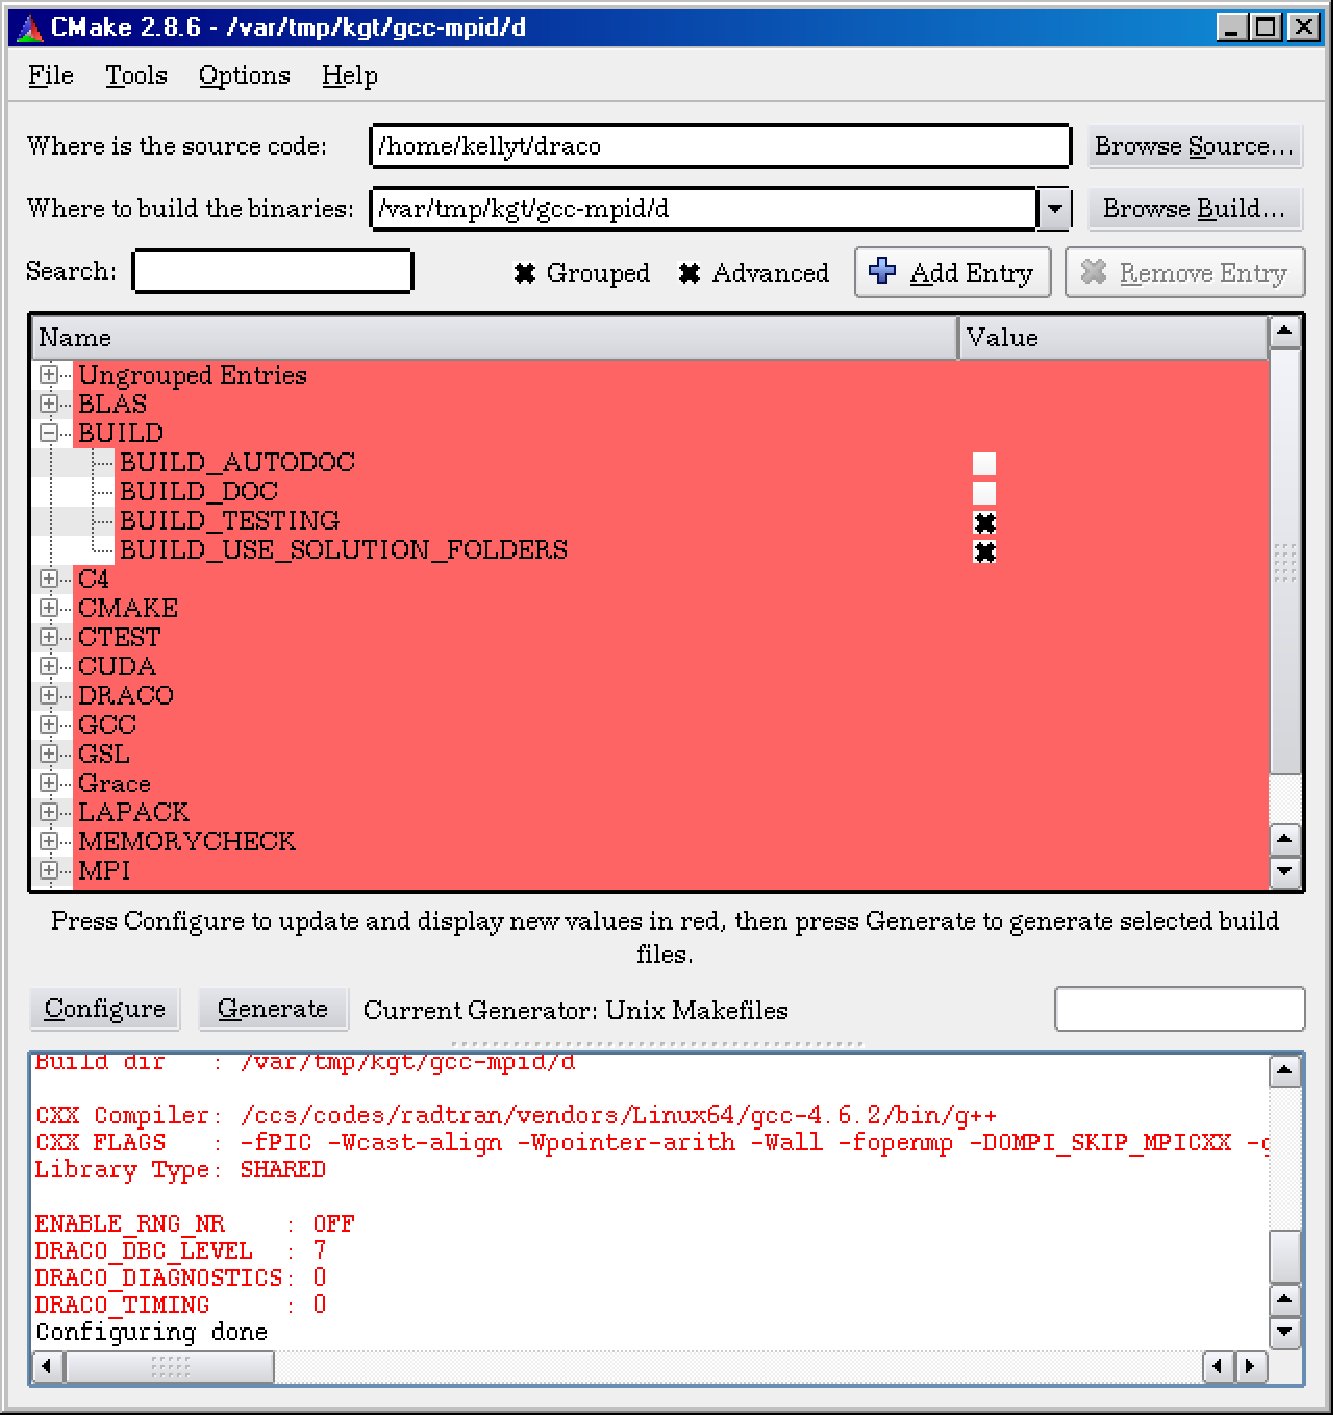
\includegraphics[angle=0,width=5.5in]{fig/cmakegui_defaults}}
  \caption{CMake GUI after populating cache with default values.}
  \label{fig:cmakegui_defaults}
\end{figure}
%

%% ---------------------------------------------------------------------------- %%
\subsection{Configuration Options}
\label{sec:configuration_options}

Because \draco\ has many packages it must support many configurations.
Additionally, some of these options can be matrixed.  For example,
\draco\ can be configured for 64-bit or 32-bit machines, scalar or parallel, with shared libraries or
archived libaries, and so forth.  The options that one gives during the \cmake\ 
configure step specify most of these options. Also, the build
system has built-in intelligence that will try to make the right
choice if incomplete listings for various options are specified.

For the standard set of \cmake\ options, see Ref.~\cite{cmake}.  The full set of configure options may be examined by running the \cmake\ interactive sessions (\comp{ccmake} or \comp{cmake-gui}).  Some options may only appear on specific systems, after specific vendor installations are discovered, or for specific {\it generators}.  This is the reason that you may need to run {\it configure} more than once when using the interactive versions of \cmake.
%For the standard set of configure options, see Ref.~\cite{autoconf}.
%The full set of configure options may be reproduced at the
%command-line by entering
%\begin{verbatim}
%     $ $draco_home/draco_config --help
%\end{verbatim}
%or 
%\begin{verbatim}
%     $ $draco_home/configure --help
%\end{verbatim}
%Note that from this point onward, we will only give examples using
%\dracoconf. 
As mentioned in the previous section, the built-in configure variable, \comp{CMAKE\_INSTALL\_PREFIX}, should be set explicitly (usually to the target directory) by the
user to avoid installation of \draco\ components in \comp{/usr/local/}.  Alternately, the developer may consider the use of \cmake's \comp{DESTDIR} feature (See \href{http://www.cmake.org/Wiki/CMake_FAQ#Does_CMake.27s_.22make_install.22_support_DESTDIR.3F}{CMake FAQ}).

Configuration options come in four forms: \comp{FILEPATH}, \comp{PATH}, \comp{STRING} and \comp{BOOL}\footnote{There are actually variable types in \cmake.  The 5th type is \comp{INTERNAL}, but this type is not available for user manipulation.}.\index{cmake!variable types}   \draco\ policy is to name \comp{BOOL} options prefixed with \comp{ENABLE\_} or \comp{USE\_}, although there are some exceptions to this policy and this policy is not adopted by \cmake\ built-in variables.  Other variable names should be prefixed with a name to provide context.  This provides a sorted in list the \comp{CMakeCache.txt} file and in the \comp{ccmake} interface and it allows groupings to be collapsed in the GUI.  This policy of using prefix context strings is a \cmake\ and a \draco\ policy standard.
Table~\ref{tab:draco-enable} lists the complete set of \comp{BOOL}
\begin{table}
  \caption{List of \comp{BOOL} options that are unique to \draco.}
  \label{tab:draco-enable}
  \begin{center}
    \begin{tabular}{lcp{3in}} \hline\hline
      \multicolumn{1}{c}{Option} & \multicolumn{1}{c}{Default Value} &
      \multicolumn{1}{c}{Description} \\ \hline
                                % --enable-shmem
%      \comp{--enable-shmem} & off & turns on \shmem\ communication
%      library \\
                                % --enable-pcglib
%      \comp{--enable-pcglib} & on & turns off \pcglib \\
                                % --enable-shared
%      \comp{--enable-shared} & off & turns on shared (\comp{.so})
%      libraries \\
%                                % --enable-static-ld
%      \comp{--enable-static-ld} & off & tries to use static
%      (\comp{.a}) libraries for linking \\
%                                % --enable-strict-ansi
%      \comp{--enable-strict-ansi} & on & compiles using \comp{strict}
%      flags for ANSI compliance \\
%                                % --enable-debug
%      \comp{--enable-debug} & off & turns on \comp{-g} option for
%      debugging$^{\text{a}}$ \\ 
%                                % --enable-32-bit
%      \comp{--enable-32-bit} & off & turns on 32-bit compiling on SGIs 
%      \\
\comp{ENABLE\_RNG\_NR} & OFF & Selects the non-reproducible random number generator feature \\
\comp{USE\_OPENMP} & ON & Disables OpenMP pragmas when compiling \draco\ sources \\
\comp{BUILD\_AUTODOC} & OFF & Enables discovery of Doxygen and the \comp{autodoc} build target \\
%\comp{BUILD_DOC} & OFF & Enables building of all \LaTeX\ documentation found in the \comp{doc} directory \\
\comp{BUILD\_TESTING} & ON & Allows developers to omit configuring for and building code found in test directories (disables \ctest\ features) \\
\comp{BUILD\_USE\_SOLUTION\_FOLDERS} & ON & Only available for \sys{Visual Studio} and \sys{X-Code} generators; makes each \draco\ component a solution folder \\
\comp{CMAKE\_VERBOSE\_MAKEFILE}$^{\text{a}}$ & OFF & Forces the make process to echo all commands to the screen during the build process \\
\comp{GCC\_ENABLE\_ALL\_WARNINGS} & OFF & When using gcc, enable more compiler warning features \\
\comp{GCC\_ENABLE\_GLIBCXX\_DEBUG} & OFF &  When using gcc, use alternate glibc library that provides bounds checking and more safety features \\

              \hline\hline
% footnote
      \multicolumn{3}{p{6in}}{$^{\text{a}}${\footnotesize this option is provided by \cmake\ and is not unique to \draco.  It is provided here because it is a commonly used feature.}}
                                % footnote
%      \multicolumn{3}{l}{$^{\text{a}}$the \KCC\ compiler automatically 
%        includes \comp{-g} support for optimization level \comp{K0},
%        see \S~\ref{sec:optimization}.}
    \end{tabular}
  \end{center}
\end{table}
switches that are unique to \draco.  To turn off a switch the user has
two options, \comp{-DENABLE\_SWITCH=OFF} or run an interactive \cmake\ session and toggle the value.  See Ref.~\cite{cmake} for more details concerning \cmake\ variables.

The \comp{PATH}, \comp{FILEPATH} and \comp{STRING} \cmake\ configure options take actual string arguments.
Table~\ref{tab:draco-with} lists commonly used argument based configure options for \draco.  Some of these are restricted to values provided by a drop down list in the GUI.
\begin{table}
  \caption{List of value based options that are unique to \draco.}
  \label{tab:draco-with}
  \begin{center}
    \begin{tabularx}{\linewidth}{
        >{\setlength{\hsize}{1.0\hsize}}X %
        >{\setlength{\hsize}{.6\hsize}}X %
        >{\setlength{\hsize}{.6\hsize}}X  %
%        >{\setlength{\hsize}{1.1\hsize}}X %
        >{\setlength{\hsize}{1.7\hsize}}X}
      \hline\hline
                                % TABLE HEADINGS
      \multicolumn{1}{c}{Option} & \multicolumn{1}{c}{Valid Arguments} 
      & \multicolumn{1}{c}{Default Value} 
%      & \multicolumn{1}{c}{Implied Argument} 
& \multicolumn{1}{c}{Description} \\ 
\hline\hline
%                                % --with-mpi
%      \comp{--with-mpi} & \comp{vendor mpich} & \comp{no} &
%      \comp{vendor} & see \S~\ref{sec:vendor_libs} \\
%                                % --with-mpi-inc
%      \comp{--with-mpi-inc} & \vble{dir} & \cnull &
%      \comp{\$MPI\_\,INC\_\,DIR} & see \S~\ref{sec:vendor_libs} \\ 
%                                % --with-mpi-lib
%      \comp{--with-mpi-lib} & \vble{dir} & \cnull &
%      \comp{\$MPI\_\,LIB\_\,DIR} & see \S~\ref{sec:vendor_libs} \\
%                                % --with-shmem-inc
%      \comp{--with-shmem-inc} & \vble{dir} & \cnull &
%      \comp{\$SHMEM\_\,INC\_\,DIR} & see \S~\ref{sec:vendor_libs} \\ 
%                                % --with-shmem-lib
%      \comp{--with-shmem-lib} & \vble{dir} & \cnull &
%      \comp{\$SHMEM\_\,LIB\_\,DIR} & see \S~\ref{sec:vendor_libs} \\
%                                % --with-sprng
%      \comp{--with-sprng} & \comp{lfg lcg} & \comp{lfg} & \comp{lfg} &
%      see \S~\ref{sec:vendor_libs} \\
%                                % --with-sprng-inc
%      \comp{--with-sprng-inc} & \vble{dir} & \cnull & 
%      \comp{\$SPRNG\_\,INC\_\,DIR} & see \S~\ref{sec:vendor_libs} \\ 
%                                % --with-sprng-lib
%      \comp{--with-sprng-lib} & \vble{dir} & \cnull &
%      \comp{\$SPRNG\_\,LIB\_\,DIR} & see \S~\ref{sec:vendor_libs} \\
%                                % --with-pcglib-lib
%      \comp{--with-pcglib-lib} & \vble{dir} & \cnull &
%      \comp{\$PCGLIB\_\,LIB\_\,DIR} & see \S~\ref{sec:vendor_libs} \\
%                                % --with-c4
%      \comp{--with-c4} & \comp{scalar mpi shmem} & \comp{scalar} &
%      \comp{scalar} & see \S~\ref{sec:c4_lib} \\
%                                % --with-dbc
%      \comp{--with-dbc} & \comp{0,1,...,7} & \vble{default} &
%      \vble{default} & see \S~\ref{sec:dbc} \\
%                                % --with-opt
%      \comp{--with-opt} & \comp{0,1,2,3} & \comp{0} & \comp{0} & see
%      \S~\ref{sec:optimization} \\
%                                % --with-posix
%      \comp{--with-posix} & \vble{posix src. num.} & \comp{199309L} &
%      \comp{199309L} & sets POSIX source version \\
%                                % --with-mips
%      \comp{--with-mips} & \comp{1,2,3,4} & \comp{mips4} & \comp{4} &
%      sets instruction set on SGIs \\
      	
      \comp{NUMDIFF} & \comp{FILEPATH} to \sys{numdiff} & automatic discovery &  tool used by testing system for comparing output to gold standard output. \\
      \comp{VENDOR\_DIR} & \comp{PATH} & empty & location used by build system for auto discovery of vendor software. \\
      \comp{DRACO\_C4} & MPI or SCALAR & MPI$^{\text{a}}$ & see \S~\ref{sec:vendor_libs} \\
      \comp{DRACO\_DBC\_LEVEL} & 0-7 & 7$^{\text{b}}$ &  see \S~\ref{sec:dbc} \\
      \comp{DRACO\_DIAGNOSTICS} & 0-7 & 0 &  see \S~\ref{sec:diagnostics} \\
      \comp{DRACO\_LIBRARY\_TYPE} & STATIC or SHARED & SHARED &  toggle compilation of archive or shared object (DLL) libraries \\
      \comp{DRACO\_TIMING} & 0-2 & 0 &  see \S~\ref{sec:diagnostics} \\
      \comp{DRACO\_VERSION} & \comp{STRING} & hard coded$^{\text{c}}$ & string that represents the current version of \draco.  This is embedded into the installed \draco\ products. \\
      \comp{DRACO\_VERSION\_FULL} & \comp{STRING} & hard coded$^{\text{c}}$ & string that represents the current version of \draco.  This is embedded into the installed \draco\ products. \\
      
      \hline
      
      \comp{CMAKE\_BUILD\_TYPE} & Debug or Release or RelWithDebInfo or MinSizeRel & Debug & choose type build type; default compiler flags are triggered based on this selection. \\
      \comp{CMAKE\_CXX\_COMPILER} & \comp{FILEPATH} to compiler & \comp{\$ENV{CXX}} & \cpp\ compiler chosen for build.\\
      \comp{CMAKE\_C\_COMPILER} & \comp{FILEPATH} to compiler & \comp{\$ENV{CC}} & C compiler chosen for build. \\
      \comp{CMAKE\_Fortran\_COMPILER} & \comp{FILEPATH} to compiler & \comp{\$ENV{FC}} & Fortran compiler chosen for build. \\
      \comp{CMAKE\_INSTALL\_PREFIX} & \comp{PATH} & \comp{\${BINARY\_DIR} /target} & location for installing \draco (libraries, headers, executables, etc). \\
      
      \hline
      
      {\it VENDOR\_VARIABLE} & varies & automatic discovery & configuration of vendors is done automatically by the \draco\ build system. See \S~\ref{sec:vendor_libs}. \\
      
      \hline\hline
% footnote
      \multicolumn{4}{p{6in}}{$^{\text{a}}${\footnotesize MPI if \sys{MPI} can be found, otherwise SCALAR.}} \\
      \multicolumn{4}{p{6in}}{$^{\text{b}}${\footnotesize The default is 7 for DEBUG builds and 0 for RELEASE (optimized) builds.}} \\
      \multicolumn{4}{p{6in}}{$^{\text{c}}${\footnotesize The version string is built from hard coded values \comp{DRACO\_VERSION\_MAJOR} and \comp{DRACO\_VERSION\_MINOR} hard coded in the top level \comp{CMakeLists.txt}. The patch revision number is set to the configure date for development builds.  Scripts used for releases set the patch version manually.}} 
    \end{tabularx}
  \end{center}
\end{table}
Notice that the build system will automatically populate all fields with default values so that \draco\ can be configured without supplying values for every possible feature.
%\comp{--with} can be used without arguments.  In this case
%an implied argument is assumed by configure.  Thus, \comp{--with}
%options have a default value and an implied argument value.  In the
%first case, a default value is inferred by configure if the
%\comp{--with} option is absent.  In the latter case, an implied
%argument is provided if the \comp{--with} option is present but does
%not specify an argument.
For example, the following two configurations are equivalent because the default value for \comp{DRACO\_C4} is \comp{MPI} if \sys{MPI} can be found on the local system.
\begin{verbatim}
     $ cmake -DDRACO_C4=MPI $draco_home
     $ cmake $draco_home 
\end{verbatim}
In each case, the \cfour\ package is configured for parallel operation with \sys{MPI}.  In the first
case an explicit argument is given.  In the second case  the default value for
\comp{DRACO\_C4} is used.  Not all cases have the same defaults for
options and arguments.  An example is the \comp{MPI\_LIBRARY}
option.  The default is the value returned from the \cmake\ built-in function \comp{find\_package(MPI)}.  For more information about configuring and auto-discovery of vendor software see \S~\ref{sec:vendor_libs} below.
% If the option is given without an argument, configure sets
%\comp{--with-mpi-inc=\$MPI\_\,INC\_\,DIR}. In general, the class of
%\comp{--with} options that load external libraries work in this
%fashion.  Most other \comp{--with} options have the same defaults as
%implied arguments.  On a final note, we do not recommend the practice
%of setting \comp{--without} because \comp{--with} options are not
%meant for binary-type operations.  An exception to this rule is the
%vendor-associated options described in \S~\ref{sec:vendor_libs}.


%% ---------------------------------------------------------------------------- %%
\subsubsection{Vendor Libraries}
\label{sec:vendor_libs}

\draco\ uses external vendors whenever possible to reduce the ammount
of code development required by \draco\ package developers.  The
following vendors are used by \draco:
\begin{itemize}
\item \mpi\ communication library, see \S~\ref{appsec:mpi};
\item \pkg{GSL}, GNU Scientific Library, provides a wide range of mathematical routines such as random number generators, special functions and least-squares fitting, see \S~\ref{appsec:gsl};
\item \pkg{LAPACK} and \pkg{BLAS} provide optimized linear algebra algorithms, see \S~\ref{appsec:lapack};
\item \pkg{CUDA} provides support for running threads on Graphic Processing Units, GPUs, see \S~\ref{appsec:cuda};
\item \pkg{DaCS} provides support for running threads on IBM cell processing units, see \S~\ref{appsec:dacs};
\item \pkg{XMGRACE} provides a 2D plotting capability, see \S~\ref{appsec:grace};
%\item \shmem\ communication library, see \S~\ref{appsec:shmem};
%\item \sprng\ random number library, see \S~\ref{appsec:sprng};
%\item \pcglib\ parallel conjugate gradient solver, see  \S~\ref{appsec:pcglib}.
\end{itemize}\index{vendor!MPI}\index{vendor!GSL}\index{vendor!LAPACK}\index{vendor!CUDA}\index{vendor!Grace}
Vendors are accessed through the \draco\ build system via automatic discovery.  
%using defined \comp{--with} and \comp{--enable} tags in \autoconf.
Table~\ref{tab:vendortags} lists the environment and build system variables that can be manipulated by the developer to alter the discovery process.
\begin{table}
  \caption{Environment and build system variables used to specify vendors in \draco.  See Tables~\ref{tab:draco-enable} and \ref{tab:draco-with} for variable defaults.}
  \label{tab:vendortags}
  \begin{center}
    \begin{tabular}{lap{3.5in}}
    \hline\hline
      \multicolumn{1}{c}{Vendor} & \multicolumn{1}{c}{Variable} & \multicolumn{1}{c}{Details} \\
      \hline
% MPI
      \mpi$^{\text{a}}$ & ENV\{PATH\} & The build system looks for \comp{mpirun} in the current \comp{PATH}. \\
      & MPIEXEC & The full path to the \comp{mpirun} program.  This may need to be set manually if the program has a non standard name like \comp{aprun}. \\
      & MPIEXEC\_NUMPROC\_FLAG & The string used to specify then number of processors to use. Defaults to \comp{'-np'}. \\ 
      & MPI\_C\_LIBRARIES & Manually specify the full paths to \sys{MPI} libraries. \\
      & MPI\_CXX\_LIBRARIES  & \\
      & MPI\_Fortran\_LIBRARIES & \\
      & MPI\_C\_INCLUDE\_PATH & Manually specify the full path to the \sys{MPI} include directory. \\
      & MPI\_CXX\_INCLUDE\_PATH & \\
      & MPI\_Fortran\_INCLUDE\_PATH & \\
      \hline
% LAPACK/BLAS      
      \pkg{LAPACK} & BLA\_STATIC & Look for archive (static) \pkg{LAPACK} and \pkg{BLAS} libraries. Default is ON. \\
      & BLA\_VENDOR & Use a particular type of \pkg{LAPACK} installation like \sys{ATLAS} or \sys{Intel10\_64lp\_gf\_sequential}$^{\text{b}}$. \\
      & ENV\{LD\_LIBRARY\_PATH\} & To help the build system find \pkg{LAPACK}, ensure that the library location is appended to this environment variable. \\ 
      & ENV\{LAPACK\_LIB\_DIR\} & To load a specific \pkg{LAPACK}, ensure this variable is set to the desired location. \\
      \hline
% GSL
      \pkg{GSL} & ENV\{GSL\_INC\_DIR\} & Help the build system find the desired installation by setting this environment variable. \\
      &  ENV\{GSL\_LIB\_DIR\} & Help the build system find the desired installation by setting this environment variable. \\
      \hline
% XMGRACe
      \pkg{XMGrace} & ENV\{GRACE\_INC\_DIR\} & Help the build system find the desired installation by setting this environment variable. \\
      &  ENV\{GRACE\_LIB\_DIR\} & Help the build system find the desired installation by setting this environment variable. \\
      \hline
% CUDA
     \pkg{CUDA}$^{\text{c}}$ &  ENV\{PATH\} & The build system looks for \comp{nvcc} in the current \comp{PATH}. \\
     & CUDA\_NVCC\_FLAGS & Modify the \comp{nvcc} compiler flags. Default is \comp{'-arch=sm\_21'}. \\
     & CUDA\_TOOLKIT\_ROOT\_DIR & If the build system cannot find \comp{nvcc}, the developer must set this location to enable \pkg{CUDA}. \\
     & CUDA\_BIN\_PATH & To use a non-standard location, set this before running \cmake. \\
     
% SHMEM
%      \shmem & --enable-shmem \\
%      & --with-shmem-inc \\
%      & --with-shmem-lib \\ \hline
% SPRNG
%      \sprng & --with-sprng \\
%      & --with-sprng-inc \\
%      & --with-sprng-lib \\ \hline
% PCGLIB
%      \pcglib & --enable-pcglib \\
%      & --with-pcglib-lib \\
      \hline\hline
      % footnotes
      \multicolumn{3}{p{6in}}{$^{\text{a}}${\footnotesize Run \comp{'cmake --help-module FindMPI'} for more details on the discovery process for \pkg{MPI}.}} \\
      \multicolumn{3}{p{6in}}{$^{\text{b}}${\footnotesize To obtain a list of support installations of \pkg{LAPACK}, see the documentation for \cmake's \comp{FindLAPACK.cmake} module (try \comp{'cmake --help-module FindLAPACK'}).}} \\
      \multicolumn{3}{p{6in}}{$^{\text{c}}${\footnotesize Run \comp{'cmake --help-module FindCUDA'} for more details on the discovery process for \pkg{CUDA}.}} \\
    \end{tabular}
  \end{center}
\end{table}
Tables~\ref{tab:draco-enable} and \ref{tab:draco-with} list additional controls that can manipulate how each vendor is used in \draco.  Details on how to use
these variables are given below.

\draco\ vendor libraries are of two types; \latin{required} and
\latin{optional}.  The type classification for each vendor is found in
Table~\ref{tab:vendor}.  \draco\ treats vendors according to the
following rules:
\begin{enumerate}
\item Required vendor libraries are on by default and the configuration will {\bf fail} if the libraries cannot be located;
\item Optional vendor libraries are on by default but the configuration will {\bf pass} if the libraries cannot be located.
\end{enumerate}
For example, \pkg{GSL} is a required vendor.  If \pkg{GSL} cannot be found, the project will not be configured and  cannot be built.  If the optional vendor \pkg{XMGrace} cannot be found, the configuration will be successful, but the \draco\ component \pkg{plot2D} will be omitted because it requires \pkg{XMGrace}.  Finally, if the optional vendor \pkg{MPI} cannot be found the configuration will be sucessful, but the \cfour\ component will be built with the \comp{SCALAR} option instead of \comp{MPI}.  Review Table~\ref{tab:depends} to determine what components may be omitted when vendor libraries are not found. This concept applies to all vendor libraries.

%We note that these rules are applied on a package-by-package basis.
%For example, \sprng\ is only required for \rng; thus, \sprng\ is on in
%the \rng\ and \imc\ packages (see Table~\ref{tab:depends}).  It is
%undefined everywhere else.  

%As illustrated in Table~\ref{tab:vendortags}, vendor options are set
%by the following three configure tags:
%\begin{enumerate}
%\item \comp{--with-\vble{vendor}} (\comp{--enable-\vble{vendor}})
%  turns the vendor on or off.  If the vendor has options (e.g.
%  \comp{--with-mpi}) then \comp{--with} is used.  If the vendor is
%  simply on or off (e.g.  \comp{--enable-shmem}) then \comp{--enable}
%  is used.
%\item \comp{--with-\vble{vendor}-inc} overrides the default \soft{cpp}
%  search locations for header files if the vendor is on.
%\item \comp{--with-\vble{vendor}-lib} overrides the default search
%  path (\ldlib) for libraries if the vendor is on.
%\end{enumerate}
%Optional vendors may be turned on simply by setting
%\comp{--with-\vble{vendor}-inc} or \comp{--with-\vble{vendor}-lib}.
%If these tags are set without setting \comp{--with-\vble{vendor}} then
%the optional library is turned on, and \comp{--with-\vble{vendor}}
%takes the value of its implied argument.  Libraries that use a
%\comp{--enable} tag are simply on in this case.  Naturally, the
%headers and libraries are searched in the directories given by
%\comp{--with-\vble{vendor}-inc} and \comp{--with-\vble{vendor}-lib}.
%For required vendors, setting \comp{--with-\vble{vendor}-inc} or
%\comp{--with-\vble{vendor}-lib} simply changes the default search
%locations for headers and libraries as explained above.

% We note that if an optional vendor is not found by the build system then
% the packages that depend on these vendors will not build.  
%%In other
%%words, required vendors need not be turned off even if the packages
%%that use them are not part of a specific \draco\ distribution.
% \draco\ knows what packages require what vendors, so optional vendor libraries that are missing
% in a particular distribution will have no effect on the rest of the packages.

%% ---------------------------------------------------------------------------- %%
\subsubsection{C4 Package Options}
\label{sec:c4_lib}

\cfour\ is \draco's parallel communication package.  It uses \mpi\ 
%either \mpi\ or \shmem\ 
to perform message passing operations.  Therefore, \cfour\ is intimately connected to the \mpi\ 
%and \shmem\ 
vendor.  The \cmake\ variable \comp{DRACO\_C4} determines how \cfour\ should be configured. 
The default option and implied argument is \comp{DRACO\_C4=MPI} when an \sys{MPI} installation is located by the build system.  However, if \cfour\ is set to \comp{SCALAR} 
then that vendor will be turned off with their implied
argument settings.  Of course, the implied arguments can be overridden by using the \mpi\ 
% or \shmem\ 
build system variables from
Table~\ref{tab:vendortags}.  In summary, if \cfour\ is set to
\comp{mpi}, those libraries will be turned on with all 
default settings.  However, any of the defaults can be changed by
using the \mpi\ vendor tags that are listed in
Table~\ref{tab:vendortags}. 

Some \sys{MPI} installations for ASC hardware are not fully supported by \cmake's built in \comp{FindMPI.cmake} routines.  
This is the case for \latin{Cielito} and \latin{Cielo}.  For these systems the \draco\ build system
employs a \latin{toolchain} file to aid in the selection of appropriate compilers and \sys{MPI} environment variables.  
To configure \draco\ on these systems use a command similar to
\begin{verbatim}
     $ cmake -DCMAKE_TOOLCHAIN_FILE=$draco_home/config/Toolchain-catamount.cmake \
             $draco_home
\end{verbatim}
The \comp{CMAKE\_TOOLCHAIN\_FILE} command line argument should appear first in the list of arguments provided to \cmake.
It is recommended that developers review the \comp{Toolchain-catamount.cmake} file to observe how the compilers and \sys{MPI}
libraries are set before compiling on either of these systems.

%% ---------------------------------------------------------------------------- %%
\subsubsection{Design-by-Contract}
\label{sec:dbc}\index{Design-by-Contract}

The \comp{DRACO\_DBC\_LEVEL} variable controls \draco's Design-by-Contract
(DBC) machinery\index{Design-by-Contract}\index{DBC}.  DBC support ranges from \comp{0} (lowest) to
\comp{7} (highest).  The value is a bit mask similar to that used by the \sys{UNIX} command \comp{chmod}, \comp{+1} turns on \comp{Require}, 
\comp{+2} turns on \comp{Check} and \comp{+4} turns on \comp{Ensure}.  If all options are activated, the  Design-by-Contract is 7. 
Table~\ref{tab:dbc} shows the DBC level for various settings of \comp{DRACO\_DBC\_LEVEL}. \index{configure options!DRACO\_DBC\_LEVEL}
\begin{table}
  \caption{DBC support in \draco.}
  \label{tab:dbc}
  \begin{center}
    \begin{tabular}{ca} \hline\hline
      \multicolumn{1}{c}{DBC Setting} & \multicolumn{1}{c}{DBC Functions} \\ \hline
      0 & None\\
      1 & Require, Remember \\
      2 & Check, Remember \\
      3 & Check, Require, Remember \\
      4 & Ensure, Remember \\
      5 & Ensure, Require, Remember \\
      6 & Ensure, Check, Remember \\
      7 & Ensure, Check, Require, Remember \\ 
      \hline\hline
    \end{tabular}
  \end{center}
\end{table}
If this option is not explicitly set by the developer (\comp{DRACO\_DBC\_LEVEL} is not defined) then the
\dsxx\ package automatically sets DBC to \comp{7}, its highest
setting, for \sys{Debug} configrations.  For \sys{Release} configurations, the DBC will be defaulted to \comp{0}, no DBC checking.  
For more information on the \dsxx\ package DBC and assertion components, see the \dsxx\ source documentation.

%% ---------------------------------------------------------------------------- %%
\subsubsection{Diagnostics}
\label{sec:diagnostics}\index{configure options!DRACO\_DIAGNOSTICS}\index{configure options!DRACO\_TIMING}

The \comp{DRACO\_DIAGNOSTICS} and \comp{DRACO\_TIMING} build variables control \draco's \pkg{diagnostic} machinery.  The purpose of this component is allow other \draco\ components to collect and report diagnostic data during runtime.  When \comp{DRACO\_DIAGNOSTICS} feature is turned off, the inserted diagnostic code does not cause any performance penalty because it is a compile time feature.  The same is true for \comp{DRACO\_TIMING} which focuses on profiling and reporting perfomance timing statistics.  The allowed values for each of these build variables are bit masks as explained in \S~\ref{sec:dbc}.  Tables~\ref{tab:ddiagnostics} and \ref{tab:dtiming} provide a description for variouls settings.
\begin{table}
  \caption{Diagnostics support in \draco.}
  \label{tab:ddiagnostics}
  \begin{center}
    \begin{tabular}{ca} \hline\hline
      \multicolumn{1}{c}{Diagnostic Setting} & \multicolumn{1}{c}{Diagnostic level description} \\ \hline
      0 & all off\\
      1 & low cost diagnostics enabled \\
      2 & moderate cost diagnostics enabled \\
      3 & moderate and low cost diagnostics enabled\\
      4 & high cost diagnostics enabled\\
      5 & high and low cost diagnostics enabled \\
      6 & high and moderate cost diagnostics enabled \\
      7 & all diagnostics enabled \\ 
      \hline\hline
    \end{tabular}
  \end{center}
\end{table}
%
\begin{table}
  \caption{Timing diagnostic support in \draco.}
  \label{tab:dtiming}
  \begin{center}
    \begin{tabular}{ca} \hline\hline
      \multicolumn{1}{c}{Timing Diagnostic Setting} & \multicolumn{1}{c}{Timing diagnostic functions} \\ \hline
      0 & all off\\
      1 & TIMER, TIMER\_START, TIMER\_STOP and TIMER\_RECORD available \\
      2 & all functions available, including TIMER\_REPORT \\
      \hline\hline
    \end{tabular}
  \end{center}
\end{table}

%% ---------------------------------------------------------------------------- %%
\subsubsection{Optimization}
\label{sec:optimization}\index{optimization}

The optimization flags\index{optimization} for the \comp{CXX}, \comp{CC} and \comp{FC} \index{configure option!CXX} \index{configure option!CC}\index{configure option!FC} compilers have default values established 
based on the compiler vendor and the selected build type (\comp{Release}, \comp{Debug}, etc.).  These flags
are established in \draco\ build system's configuration files \comp{config/}\vble{arch\_compiler\_vendor}\comp{.cmake} 
(e.g.: \comp{config/unix-g++.cmake} or \comp{config/windows-cl.cmake}).  In general, \comp{Release} configurations will use optimization flags like \comp{-O3 -funroll-loops} and \comp{Debug} configurations will include debug symbols and no optimization, \comp{-g -O0}.  The \comp{RelWithDebInfo} configuration uses a mixture of flags trying to produce an optimized configuration that still has the debug symbols.  \draco\ policy to keep the source code as close to the language standard as possible.   To aid the developer, the \comp{Debug} configurations impose compiler flags that will increase the warning level and verbosity during the compilation.  For example, when using the \sys{g++} compiler the flags \comp{'-ansi -pedantic -Wcast-align -Wpointer-arith -Wall'} are used for \comp{Debug} configurations. In general, \comp{Release} builds use the most aggressive optimizations that provide reliable and consistent results.

%The optimization flags for \KCC, the \cpp\ compiler of choice for
%\draco, has some unique options.  Specifically, the lowest level of
%optimization, \comp{--with-opt=0}, which is given by default and by
%implied argument, automatically sets the \KCC\ compile-line flag,
%\comp{+K0}.  The \comp{+K0} option implicitly includes the debug flag
%\comp{-g}.  Thus, when \comp{--with-opt=0} the debug flag
%(\comp{--enable-debug}) does not have to included.  \draco\ has
%built-in intelligence that will turn off the \comp{-g} flag if the
%\KCC\ optimization is set to \comp{0}.  The \comp{-g} flag will be
%included for any optimization setting greater than \comp{0}.

%%---------------------------------------------------------------------------%%

\section{Building Draco}
\label{sec:building_draco}

After configuration, building \draco\ is mostly straightforward.  For \sys{UNIX} \sys{Makefile} build configurations, 
one simply enters the binary directory, or a component's binary
subdirectory, and runs \gmake.  The \draco\ Makefiles include all of
the standard targets provided by \cmake.  For more detail, see ref.~\cite{cmake}. The most commonly used targets are \comp{all} and \comp{install}.  \index{build target!all}\index{build target!install}
The \draco\ build system takes full advantage of multi-core architectures allowing multithreaded compilation of \draco.  
To take advantage of this features use the \comp{'-j N'} option of \gmake.  The recommended value for the number of concurrent threads, 
\comp{N}, is 50\% oversubscription of the number of available cores (i.e.: 24 for a 16-core machine). Examples of various builds are reserved
until \S~\ref{sec:examples}.\index{compile!parallel}

For other build environments like \sys{Eclipse} or \sys{XCode}, \cmake\ provides a solution configuration that can be loaded into the IDE.  Use the 
build environment's normal methods for compiling the \comp{ALL\_BUILD} target.

%% ---------------------------------------------------------------------------- %%
\subsection{Building and Installing}

Building and installing \draco\ is specific to each generated project type.  The following subsections provide details for the most commonly used development environments.

\subsubsection{Unix Makefiles}

To build and install \draco\ simply enter the \comp{\vble{target}/draco/} binary directory and run \comp{'gmake -j'}.  At this
level, \gmake\ will enter each subdirectory under \comp{\vble{target}/draco/} and do a full build.
% followed by an install.  
The default targets in subdirectories under \comp{\vble{target}/draco/} are the same as at the top level.  It should be noted that the default target, \comp{all}, does not run unit tests or install \draco\ libraries or headers.  You must run \comp{'make -j install'} to tell the build system to copy the installable artifacts to the prefix directory.
%  Table~\ref{tab:gmake} shows   the default targets at various
%\begin{table}
%  \caption{Default targets for \gmake\ at each directory level.  The
%    \comp{draco/} directory is a subdirectory of the target directory.}
%  \label{tab:gmake}
%  \begin{center}
%    \begin{tabularx}{\linewidth}{
%        >{\setlength{\hsize}{.85\hsize}}L %
%        >{\setlength{\hsize}{.75\hsize}}L %
%        >{\setlength{\hsize}{1.4\hsize}}X}
%      \hline\hline
%      \multicolumn{1}{Y}{\draco\ directory} &
%      \multicolumn{1}{Y}{Default Target} &
%      \multicolumn{1}{Y}{Description} \\ \hline
%                                % draco/
%      draco/ & install: & builds and installs all sub-directories \\
%                                % draco/src
%      draco/src & install: & builds and installs all \comp{src/}
%      sub-directories \\
%                                % draco/src/pkg
%      draco/src/\vble{pkg} & lib\vble{pkg}.\vble{suffix}: & builds the
%      library for \vble{pkg} \\
%                                % draco/src/pkg/test
%      draco/src/\vble{pkg}/test & \${test\_\,alltarget}: & builds all of
%      the test executables \\
%                                % draco/doc
%      draco/doc & install dvi: & builds and installs main \draco\
%      manual \\
%                                % draco/doc/sub-doc
%      draco/doc/\vble{sub-doc} & \${manual} & builds the manual
%      (\comp{.dvi}) in the \vble{sub-doc/} directory \\
%                                % draco/tools
%      draco/tools & install: & installs tools into the \comp{libexec}
%      directory specified by \comp{--prefix} \\
%      \hline\hline
%    \end{tabularx}
%  \end{center}
%\end{table}
%levels of the target directory tree.  
% If \gmake\ is run at levels lower than the \comp{\vble{target}/draco/src/} directory, the user must be aware of package dependencies.  
% For example, \cfour\ cannot be built if \dsxx\ has not been built and installed.  Thus, the general user should avoid manual builds of packages at the
% \comp{\vble{target}/draco/src/\vble{pkg}/} level.  At higher levels, \draco\ knows how to build packages in the proper order.

\subsubsection{Eclipse}
To be completed later.

\subsubsection{XCode}
To be completed later.

\subsubsection{Visual Studio}
To be completed later.

\subsubsection{Running the Tests}

Each \draco\ component provides a full suite of unit tests that demonstrate and check the component algorithm's capabilities.  \index{tests!executing}
To run the tests, run \ctest\ from any location in the binary directory.  
If \ctest\ is run from the top level, all unit tests will be run.  
If run from a component subdirectory, only the tests for that component will be executed.  
The \draco\ build system knows how to run the unit tests in parallel taking advantage of all available hardware resources.  
It is recommended that the \ctest\ command be issued with the \comp{'-j N'} option, where \comp{N} is the number of concurrent threads that should be used.  
For testing purposes, it is better to avoid over-subscription of the machine's hardware.

\ctest\ provides many options for running tests: selecting a subset of tests to run; running with different output verbosity, etc.  The developer should review the \ctest\ documentation found at Ref.~\cite{cmake} and by using the \comp{'ctest --help'} command.  In particular, the \comp{-VV} options selects full verbosity for tests and the \comp{-R} option selects all tests whose names match a provided regular expression.  It is \draco\ policy that tests names will provide both the component name and the number of MPI ranks used (if any) in the test name.  This policy allows the developer to run all \cfour\ tests by using the command\index{tests!options}
\begin{verbatim}
     $ ctest -R c4
\end{verbatim}
or all 4 processor MPI tests could be selected by the command:
\begin{verbatim}
     $ ctest -R _4
\end{verbatim}
A list of available test can be obtained using the \comp{-N} option to \ctest.

\subsubsection{Additional Observations and Features}

At each target directory level the \draco\ build system knows all of the component
dependencies so the developer can start the build at any place in the binary tree. 
For example, when compiling from the \cfour\ component directory, the build system will check to see if the \dsxx\ library has been compiled.  
If not, then the \dsxx\ library will be built before compilation of \cfour\ sources begins.  
Even in this situation the build system remains fully aware of threading and it is recommended that a parallel build process be performed unless the developer 
is trying to debug a build system error.   
This aspect of the build system is a feature for \draco\ developers.  
It allows the developer to only compile or recompile sources that are required for building the desired target.  
One drawback is that other components in parallel directories may be modified during a targeted compile and the developer should remain aware of 
these dependencies as  illustrated in Fig.~\ref{fig:level} and are listed in Table~\ref{tab:depends}.
%
%Thus, \cfour\ simply checks to see if \dsxx\ has been
%installed.  If \dsxx\ does not exist in the install location specified
%by \comp{--prefix} then \gmake\ will end.   It gives developers the
%flexibility to modify code in a package and test it without affecting
%other packages that may depend on that code.  One drawback is that
%users must be aware of the package dependencies when performing manual
%builds.  These dependencies are

%This is done to conform to the GNU Standard, which states that tests should not be dependent upon installation.  The \comp{check} target uses \dejagnu\ to generate test 
%output data and results.  For more information, see
%ref.~\cite{dejagnu}.  A future \draco\ document will describe the
%details of \draco\ regression testing.

An additional feature of the \draco\ build system is that \draco\ will automatically rerun the \cmake\ configuration step if any of the configuration system files have been modified.  
Thus, if \comp{CMakeLists.txt} or any of the files from the \comp{config} source directory are changed then the build process will first reconfigure the entire project.  

%% ---------------------------------------------------------------------------- %%
\subsection{Build Targets}
\index{build target!all}
\index{build target!install}
\index{build target!check}
\index{build target!clean}
\index{build target!rebuild\_cache}
\index{build target!test}
\index{build target!edit\_cache}
\index{build target!Experimental}
\index{build target!help}

A detailed discussion of all the build targets provided by \cmake~\cite{cmake} is beyond the scope of this text. 
What follows is a brief description of the build targets in \draco\ and what operations they perform.\index{build:targets}
\begin{description}
\item[\comp{all}]\index{gmake!target!all} (default) build all products at the current level and in all subdirectories.  If configuration files have been modified, rerun \cmake\ to reconfigure the project before compilation begins.
\item[\comp{install}]\index{gmake!target!install|textbf} build all products at the current level and in all subdirectories; then install the products in the locations specified by \comp{CMAKE\_INSTALL\_PREFIX}.  All build products are compiled before any are installed. 
\item[\comp{check}]\index{gmake!target!check|textbf} build all products at the current level and in all subdirectories; then run \ctest\ to execute all unit tests.  This target does not install any products (this behavior is different than older versions of \draco).
%\item[\comp{install dvi}]\index{gmake!target!install dvi|textbf}
%  \gmake\ will build and install the main \draco\ manual when this is
%  run from the \comp{draco/} or \comp{draco/doc/} directories.  When
%  this target is run from a \comp{draco/doc/\vble{sub-doc}/} directory
%  it will build the \vble{sub-doc} manual and install it.
%\item[\comp{dvi}]\index{gmake!target!dvi|textbf} \gmake\ will build
%  the manual in the directory where this target is run.  In
%  \comp{draco/doc/} it will build the main manual.  In
%  \comp{draco/doc/\vble{sub-doc}/} it will build the \vble{sub-doc}
%  manual.
\item[\comp{clean}]\index{gmake!target!clean|textbf} clean the compiled files (\comp{*.o}, libraries and executables) from the target sub-directories.
\item[\comp{rebuild\_cache}]\index{gmake!target!rebuild\_cache} rerun the \cmake\ configure process and regenerate all project files (e.g.: \comp{Makefiles}, \comp{config.h}, etc.).
\item[\comp{edit\_cache}]\index{gmake!target!edit\_cache} run the \cmake\ editor to allow the developer to edit the configuration variables. 
\item[\comp{test}]\index{gmake!target!test} run \ctest\ to execute all unit tests.
\item[\comp{Experimental}]\index{gmake!targets!Experimental} configure, compile, run the tests and submit the results to the \draco\ \cdash\ dashboard.
\item[\comp{Lib\_}\vble{pkg}]\index{gmake!targets!Lib\_pkg} Compile the library for \draco\ component \vble{pkg}.
\item[\comp{Ut\_}\vble{pkg\_test}\comp{\_exe}]\index{gmake!targets!Ut\_pkg\_test\_exe} Compile the unit test executable for test \vble{test} for the \draco\ component \vble{pkg}.
\item[\comp{help}] provides a list of available targets.
\end{description}
These targets have been designed to satisfy the needs of users, who
perform one-time global builds, and developers, who perform multiple
local builds.

%%---------------------------------------------------------------------------%%

\section{Recommended Practices}

Although \draco\ can be configured and built in any number of ways, we 
have a set of ``standard'' recommended practices that are followed by
\draco\ team members.  This methodology for configuring and
building \draco\ is summarized in the following steps:
\begin{enumerate}
\item Checkout a version of \draco\ from \svn; the location of which is \dracohome.
\item Make a target directory that appropriately describes the configuration options; 
we call this directory \comp{\vble{target}/}.
\item Make a \comp{draco/} binary subdirectory under the target directory,
  ie. \comp{\vble{target}/draco/}.
\item Run \cmake\ in \comp{\vble{target}/draco/} with the appropriate options for this
  configuration.  Set \comp{-DCMAKE\_}\-\comp{INSTALL\_}\-\comp{PREFIX=\vble{target}/}. Thus, the
  configure line is:
  \begin{alltt}
    $ cmake -DCMAKE_INSTALL_PREFIX=`pwd`/.. \vble{options} $draco_home 
  \end{alltt}
\item Run \gmake\ in \comp{\vble{target}/draco/};
\begin{verbatim}
    $ gmake -j install
\end{verbatim} % $
  This step will build and install all of the \draco\ products from
  each subdirectory under \comp{\vble{target}/draco/}.  The headers
  will be installed in \comp{\vble{target}/include/}.  The libraries
  will be installed in \comp{\vble{target}/lib/}. 
  And the executables will be installed in \comp{\vble{target}/bin/}.
  %And, the package-dependent executables will be installed in \comp{\vble{target}/libexec}.
\end{enumerate}
This procedure simplifies adding an external code system that uses,
and is based on, \draco.  For example, \clubimc\ uses \draco\ as a
build-model template.  Thus, we can add a \comp{\vble{target}/clubimc}
directory and configure, build, and install \clubimc\ in the same
location as \draco\ products.  Details on this process are given in
\S~\ref{sec:emulating}. 

%%---------------------------------------------------------------------------%%

\section{Examples}
\label{sec:examples}

To illucidate some of the concepts that we have described in this
chapter, we proceed to show some configuration and build examples.
The following examples give a cross section of the processes that
\draco\ users and developers will use.\index{build!examples}
\begin{cexa}
  \label{ex:basic}
  Build a scalar version of \draco\ on a \sys{Linux} platform using the \sys{Makefile} generator.  
  %\sprng\ headers are in the \soft{cpp} include path, and \sprng\ and \pcglib\ libraries are found in \ldlib.  
  \pkg{GSL} libraries are found in \ldlib.
  The \draco\ source directory is \comp{/usr/tmp/joe/draco}.  
  We want \draco\ installed in \comp{/usr/local/draco}.
\end{cexa}
\begin{proof}[Solution to \ref{ex:basic}]
  First, we need to make a target directory.  In
  \S~\ref{sec:running_configure_prepare} we advised not to use the source
  directory as the build directory.  We will follow this policy and
  make our target directory \comp{draco\_\,target}:
\begin{verbatim}
     $ cd /usr/local/draco
     $ mkdir draco_target
\end{verbatim}
  Note that we could have created a directory named \comp{draco/} instead of \comp{draco\_\,target/}.
  We used a different name to illustrate the independence of the target-build directory.  Now, we configure
  \draco\ according to the specification in Ex.~\ref{ex:basic}.  This
  configuration is scalar so we must specify alternate settings for
  \cfour.  Additionally, all of the required vendors are located in
  default locations.
\begin{verbatim}
     $ cd draco_target
     $ cmake -DCMAKE_INSTALL_PREFIX=`pwd`/.. -DDRACO_C4=SCALAR \
             /usr/tmp/joe/draco/draco_config
\end{verbatim}
  All other defaults are used except the explicit setting for \comp{DRACO\_C4}.
  Finally, we want to do a build and install of all \draco\ products;
  thus, according to \S~\ref{sec:building_draco}, we must enter
\begin{verbatim}
     $ gmake -j install
\end{verbatim} % $
  Generally, it is better run the build (\comp{all} target and then run the unit tests via \ctest\
  before running the \comp{install} target.  This gives the develper a chance to ensure that all tests
  pass before the build is installed.
\begin{verbatim}
     $ make -j 
     $ ctest -j
     $ make -j install
\end{verbatim} %   
\end{proof}

Example~\ref{ex:basic} is straightforward.  We will now give a series
of examples and solutions that involve more detailed configurations
and builds.  At this point, we will only show the steps in the
solution procedure.  The details about each step can be inferred from
\S~\ref{sec:configuring_draco} and \ref{sec:building_draco}.

\begin{cexa}
  \label{ex:mpi}
  Build a version of \draco\ with \mpi.  Additionally, this build
  takes place on a Linux platform with \sys{OpenMPI} and \sys{GSL} loaded as a modules.
%  with \comp{\$MPT\_\,SGI} loaded as a module.
%  Thus, we are using the SGI vendor version of \mpi.  \sprng\ is
%  located in \comp{/usr/local/sprng} and \pcglib\ is in the \ldlib.
\end{cexa}
\begin{proof}[Solution to \ref{ex:mpi}]
  Before proceeding to the solution, we note that the \draco\ build
  system knows about the \sys{OpenMPI} module.
  Thus, setting the include and library paths for \mpi\ is not
  required.
\begin{verbatim}
     $ cd /usr/local/draco
     $ mkdir draco
     $ cd draco
     $ cmake -DCMAKE_INSTALL_PREFIX=`pwd`/.. /usr/tmp/joe/draco .. 
     $ make -j 
     $ ctest -j
     $ make -j install
\end{verbatim} % $
\end{proof}

\begin{cexa}
  \label{ex:mpich}
  Build a version of \draco\ with \mpi\ and optimization set to level
  \comp{3}.  Turn off all DBC support.  Use the \sys{mpich} version of
  \mpi\ that is installed in \comp{/usr/local/}. 
  \sys{GSL} is in \comp{/usr/local/gsl}.  This could be considered a production
  version of \draco.
\end{cexa}
\begin{proof}[Solution to \ref{ex:mpich}]
  We will proceed in a slightly different manner than the previous
  examples.  Here we will use environment variables to determine the
  location of \sys{GSL}.  We assume the \soft{BASH} shell is in use.
\begin{verbatim}
     $ export GSL_INC_DIR=/usr/local/gsl/include
     $ export GSL_LIB_DIR=/usr/local/gsl/lib
     $ cd /usr/local/draco
     $ mkdir draco
     $ cd draco
     $ cmake -DCMAKE_INSTALL_PREFIX=`pwd`/.. -DCMAKE_BUILD_TYPE=RELEASE /usr/tmp/joe/draco 
     $ make -j
     $ ctest -j
     $ make -j install
\end{verbatim}
The \sys{MPI} setup is automatic assuming that \comp{mpirun} for \sys{mpich} is available from the environment variable \comp{PATH}.  Setting the \comp{CMAKE\_BUILD\_TYPE=RELEASE} sets the optimization level to 3 and turns off DBC.  If we had wanted to keep the DBC turned on for the optimized build, we would need to provide an additional argument to \cmake\, \comp{'-DDRACO\_DBC\_LEVEL=7'}.
\end{proof}

%%---------------------------------------------------------------------------%%

\section{Summary}

We have given a tutorial on how to configure and build \draco.  The
component and vendor dependencies in \draco\ have been listed in
\S~\ref{sec:draco_dependencies}.  Details on configuring and
building \draco\ have been given in \S~\ref{sec:configuring_draco} and 
\S~\ref{sec:building_draco}.  We have tied these concepts together with
several examples in \S~\ref{sec:examples}.

%%---------------------------------------------------------------------------%%
%% extern.tex
%%
%% how to make an external code package that uses draco fit in with
%% the draco build system
%%---------------------------------------------------------------------------%%

\chapter{Using the Draco Build Model in External Codes}
\label{chap:extern}

This chapter illustrates how to use the \draco\ and the \draco\ build
model in external code systems.  One of the advantages of \draco\ is
that it is independent from its clients.  Thus, one may use \draco\ 
without having any direct connections to its build system.  All that
is required is linking to the \draco\ libraries that one wishes to
use.  Details on how to use \draco\ as a client are given in
\S~\ref{sec:using}.

Code systems that use \draco\ heavily may find benefits in emulating
the \draco\ build model.  This prevents these systems from having to
define all of \draco's dependencies.  By using the \draco\ build
system they get the correct compile and link-line options
automatically.  We discuss how to use the \draco\ build system in
external codes in \S~\ref{sec:emulating}.

%%---------------------------------------------------------------------------%%

\section{Using Draco in External Codes}
\label{sec:using}

As mentioned in the previous section, \draco\ and external clients are
separate entities.  Thus, any build system that the external client
desires is acceptable.  This can range from a simple
``compile-script'' to a detailed \autoconf-\gmake\ build system.
Describing all possible build systems that use \draco\ is beyond the
scope of this, or any, text.  However, we will point out some useful
items that should be considered when using \draco\ as an external
client.

First, clients of \draco\ should follow the \draco\ practice of
setting include paths to the \draco\ include directory specified by
\comp{--prefix}.  Thus, headers should be included in source code
using
\begin{verbatim}
     #include "pkg/header.hh"
\end{verbatim}
For example, if a client wishes to use the \dsxx\ smart pointer class
then the client source code should contain the following:
\begin{verbatim}
     #include "ds++/SP.hh"
\end{verbatim}
The \draco\ headers are included on the compile and link-lines with
the following statement
\begin{verbatim}
     -I /usr/local/draco/include
\end{verbatim}
where \comp{/usr/local/draco} is the \draco\ installation location.
By following this convention the client will avoid name clashes among
\draco\ packages.

\draco\ clients must remember to include all dependencies for a
particular \draco\ package.  These dependencies are both implicit and
explicit for \draco\ packages and vendors.  Tables~\ref{tab:depends}
and \ref{tab:vendor} can be used to determine the full list of
dependencies for a particular \draco\ package.  Additionally, clients
must remember to include the same vendor installations as the ones
supplied to \draco.  For example, if \draco\ used an \sys{MPICH}
version of \mpi\ then the client should use the same vendor and
version when linking.

As stated in \S~\ref{sec:overview_of_draco}, \draco\ uses the generic
programming archetype.  Thus, many classes and functions in \draco\ 
are templates and are not compiled into libraries.  \draco\ does not
support implicit instantiation~\cite{ansi:cpp} of template classes and
functions.  Thus, the user must provide explicit instantiation source
code for \draco\ template components.  \draco\ template code is stored
in \comp{.t.hh} files.  These files are installed in the
\comp{include/} directory along with the rest of the \draco\ package
headers. Specific information on the generic programming approach used in 
\draco\ is given in ref.~\cite{ro98}.

%%---------------------------------------------------------------------------%%

\section{Emulating the Draco Build System}
\label{sec:emulating}

The \draco\ build system can be emulated at varying levels ranging
from full to minor.  We will describe a method for using the \draco\ 
build system directly.  If this method is used the \draco\ build
system requires little or no modification in the external system.
External code systems that utilize the \draco\ build system in this
manner are \solon, \tycho, \milagro, and \kepler.

The most direct method of incorporating the \draco\ build system into
an external product is to mimic the structure of the \draco\ source
tree.  This process has three steps:
\begin{enumerate}
\item Setup the external code source tree in the same manner as
  \draco; setup a top-level directory, a \comp{src/} directory, a
  \comp{doc/} directory, and a \comp{config} directory.  Components of 
  the code should be placed in \comp{src/\vble{pkg}/} directories.
\item copy the components from \comp{draco/config/} into the new code
  \comp{config/} directory.
\item When configuring, set the \comp{--prefix} tag to the same
  location as the installed \draco\ components.
\end{enumerate}
If these steps are followed, then the external code system should
properly attach \draco\ libraries and find \draco\ headers.  However,
the external code developer should be aware that external code
components will be installed in the same location as \draco\ 
components.

Including the \draco\ components in external components is easily
accomplished using \cvs.  Through \cvs\ module control we have
included the \comp{draco/config} directory into the \milagro\ and
\solon\ code systems.  Thus, these systems will automatically get
updates of the \draco\ build system components.  This option is only
available to \draco\ developers who have access to the \draco\ \cvs\ 
repository.

Each package subdirectory in the external code system must have a
\comp{configure.in} file as described in \S~\ref{sec:adding_overview}.
The contents of these files are described in
\S~\ref{sec:package_files}.  These files will be very similar to the
\comp{configure.in} scripts found in \draco.  The fundamental
difference is that the external code will add its own package
dependencies to the existing \draco\ dependencies.
Chapters~\ref{chap:adding} and \ref{chap:extend} go into greater
detail on package design in the \draco\ build system.

Additinally, the external code may require vendors that are not
supported by \draco.  Thus, vendor tags in addition to those shown in
Table~\ref{tab:vendortags} may need to be defined.  Defining vendors
using \draco-like methodology is described in
Chap.~\ref{chap:extend}.  

On a final note, any deviations from the \draco\ build model in an
external code system are perfectly acceptable.  The external code
client and \draco\ are independent entities.  In many cases, exactly
emulating \draco\ is the most straightforward way of incorporating
\draco\ into an external code package.  An additional benefit of
emulating the \draco\ build system is that one gains a GNU Standard
system.

%%---------------------------------------------------------------------------%%

\section{Summary}

We have given directions on how to use \draco\ in an external code
system.  In \S~\ref{sec:emulating} we have shown how to directly use
\draco\ in a code system that makes heavy use of the \draco\ component 
library.  In \S~\ref{sec:using} we have given some pointers to codes
that are \draco\ clients but simply want to link to \draco\
components without using the \draco\ build system.
%%---------------------------------------------------------------------------%%
%% adding.tex
%%
%% how to add a new package to the draco system
%%---------------------------------------------------------------------------%%

\chapter{Adding a Component to Draco\index{Draco!adding components}}
\label{chap:adding}

\section{Overview}
\label{sec:adding_overview}

New \draco\ components should be added in subdirectories under
\comp{draco/src/}.  Each \draco\ package may have its own additional
subdirectories under \comp{draco/src/\vble{pkg}}.
Figure~\ref{fig:package} illustrates a representative package
directory.  A component directory should conform to following
guidelines:
\begin{itemize}
\item each component directory should have a \comp{test/} subdirectory
    that holds component test code, these tests are also used to
    verify package builds as described in \S~\ref{sec:building_draco}. Most unit tests should use the features provided by the \comp{ds++/ScalarUnitTest} or \comp{c4/ParallelUnitTest} helper classes,
\item each component should have \comp{autodoc/}  and \comp{doc/} subdirectories.  The  \comp{autodoc/} directory should provide at least one file, \latin{pkg/}\comp{.dcc.in}, that provides basic information about the component that can be included in the compiled HTML autodoc for \draco,
\item all subdirectories in the package should have the same configuration and build options,
\item the component should use as many of the \cmake\ macros defined by the \draco\ build system as possible to avoid duplicate code,
%\item components should use the \draco\ system default
%  \comp{Makefile.package.in}\index{Makefile.package.in} and
%  \comp{Makefile.test.in}\index{Makefile.test.in} makefiles,
%\item packages should use the \draco\ system default \autoconf\ macros
%  in \comp{aclocal.m4}\index{aclocal.m4} in
%  \comp{configure.in}\index{configure.in|(},
%\item if the package has special needs, it can have a unique
%  \comp{Makefile.in}\index{Makefile.in|(},
\item special configuration requirements for a package may be added to 
  that package's \comp{CMakeLists.txt} file.
\end{itemize}
\begin{figure}[htbp]
  \begin{center}
    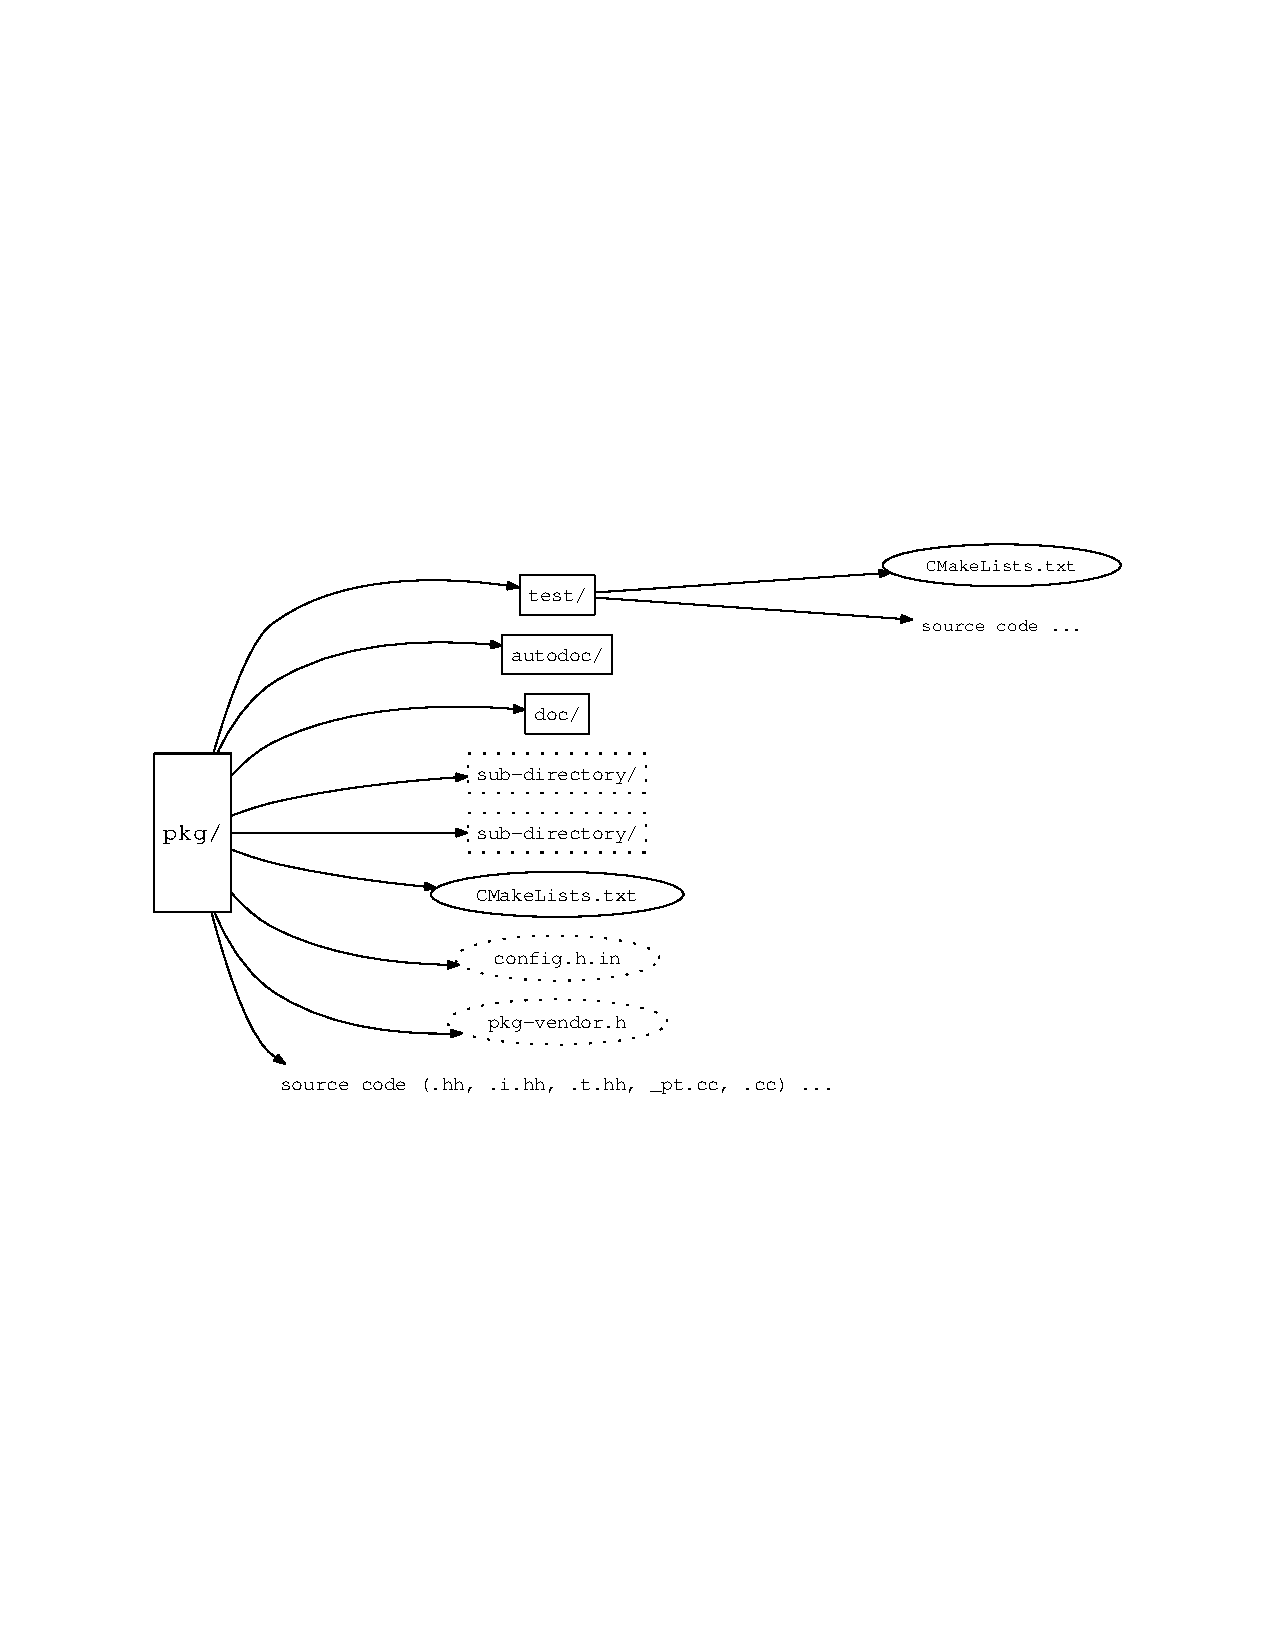
\includegraphics[clip, trim=1cm 9cm 1cm 9cm,width=6.5in]{fig/package} % trim=l b r t
    \caption{Standard package directory configuration in \draco.}
    \label{fig:package}
  \end{center}
\end{figure}
In general, most packages will be able to use another component's \comp{CMakeLists.txt} and \comp{autodoc/}\latin{pkg}\comp{.dcc.in} as a templates.  Customization of 
component \comp{CMakeLists.txt}  files is treated in \S~\ref{sec:customize}.

At a minimum, each package requires a \comp{CMakeLists.txt}.  
% Additionally, the package must have access to a makefile template.  \draco\ provides the default makefile templates \comp{Makefile.package.in} and \comp{Makefile.test.in} for
% \comp{src/\vble{pkg}/} and \comp{src/\vble{pkg}/test} directories.
To set configuration options on a package-by-package basis,
the files \comp{config.h.in}\index{config.h.in|(} and \comp{\vble{pkg}-\vble{vendor}.h}\index{pkg-vendor.h|(}, may also be required.
Table~\ref{tab:pkgfiles} lists all of the possible configuration files
\begin{table}
  \caption{\draco\ build system package files.}
  \label{tab:pkgfiles}
  \begin{center}
    \begin{tabularx}{\linewidth}{
        >{\setlength{\hsize}{.5\hsize}}L %
        >{\setlength{\hsize}{1.5\hsize}}X}
      \hline\hline
      \multicolumn{1}{Y}{Package Configuration Files} &  
      \multicolumn{1}{Y}{Description} \\
      \hline
% CMakeLists.txt
CMakeLists.txt & file contains cmake instructions for generating directly local project files (e.g.: Makefiles).      \\
                                % configure.in
%      configure.in & file containing \autoconf\ tests that is used to
%      build \comp{configure*} \\
%                                % configure*
%      configure* & package configure script generated by \autoconf\ from 
%      \comp{configure.in} \\
%                                % Makefile.in
%      Makefile.in & special package makefile, this is present only if
%      the default \comp{Makefile.package.in} is not used \\
%                                % Makefile.srcs
%      Makefile.srcs & special source modifications, called by the
%      default makefiles \\
%                                % Makefile.target
%      Makefile.target & special target modifications for package test
%      directories, called by the default makefiles \\
%                                % Makefile.misc
%      Makefile.misc & special makefile for miscellaneous additions,
%      called by the default makefiles \\
                                % config.h.in
      config.h.in & package specific environment configuration file that will be processed into \comp{\$\{PROJECT\_BINARY\_DIR\}/}\latin{pkg}\comp{/config.h} \\
                                % package-vendor.h
      \vble{pkg}-\vble{vendor}.h & package-specific vendor include  headers \\
      \hline\hline
    \end{tabularx}
  \end{center}
\end{table}
that can be found in a \draco\ package.  All of these files are
explained in \S~\ref{sec:package_files}.

\draco\ does not provide templates for package-level \comp{CMakeLists.txt} and
\comp{config.h.in} files, but the contents of these files are straight forward for most cases and the developer can use an existing component's \comp{CMakeLists.txt} and
\comp{config.h.in} files as templates.

\draco\ macros are defined in \cmake\ configuration files located at \comp{draco/config/}.  These
macros are used by \cmake\ to generate the build logic and platform checks that go into the generated project files for the selected build type (e.g: Makefiles).  
The macros are divided into separate files to provide appropriate groupings as presented in Table~\ref{tab:config_grouping}.
 \begin{center}
   \label{tab:config_grouping} 
 \begin{longtable}{p{1.0in}ap{3.1in}}
% {\linewidth}{
%        >{\setlength{\hsize}{.35\hsize}}X %
%        >{\setlength{\hsize}{1.05\hsize}}L %
%        >{\setlength{\hsize}{1.35\hsize}}X}
  \caption{Draco configuration macro files.} \\
  
      \hline\hline      
      \multicolumn{1}{c}{Type} & \multicolumn{1}{c}{Configuration File}  & \multicolumn{1}{c}{Description} \\
      \hline
      \endfirsthead
      
      \hline\hline
      \multicolumn{1}{c}{Type} & \multicolumn{1}{c}{Configuration File}  & \multicolumn{1}{c}{Description} \\
      \hline
      \endhead
      
      \hline \multicolumn{3}{r}{\textit{Continued on next page}} \\
      \endfoot
      
      \hline\hline 
      \endlastfoot
      
% FindXXX
Vendor support
& FindGSL & use \cmake's \comp{find\_package\_handle\_standard\_args} to locate and register settings for GSL. \\
& FindGrace & use \cmake's \comp{find\_package\_handle\_standard\_args} to locate and register settings for XM Grace.  \\
& FindLIBSCI & use \cmake's \comp{find\_package\_handle\_standard\_args} to locate and register settings for Cray's LibSCI (an optimized \sys{LAPACK} replacement. \\
& vendor\_libraries & controlling macro that looks for requested vendor libraries by calling \comp{find\_package()}. \\

\hline

% Toolchain      
Toolchain files
& Toolchain-catamount & allow use of \cmake's cross-compile feature to aid the build system configuration for Catamount-like systems.\\
& Toolchain-roadrunner-ppe &  allow use of \cmake's cross-compile feature to aid the build system configuration for Roadrunner cell front end. \\
& Toolchain-roadrunner-spu &  allow use of \cmake's cross-compile feature to aid the build system configuration for Roadrunner cell back end.\\
\hline

% Primary configuration setup
Primary configuration
& buildEnv & establish top-level defaults like \comp{DRACO\_DBC\_LEVEL} \\
& compilerEnv & controls compiler discovery and calls appropriate compiler flag setup routines \\
& dracoVersion & establishes the \draco\ version tag that is embedded in the code \\
& dracoTesting & establishes the \comp{check} build target. Test registration macros are provided in \comp{component\_}\-\comp{macros}\-\comp{.cmake}. \\
& platform\_checks & macros that probe the local system for available features, headers, etc. \\
& unix-g++ & sets compiler flags for GNU C and C++\\
& unix-gfortran & sets compiler flags for GNU Fortran \\
& unix-ifort & sets compiler flags for Intel Fortran \\
& unix-intel & sets compiler flags for Intel C and C++ \\
& unix-pgf90 & sets compiler flags for PGI Fortran \\
& unix-pgi & sets compiler flags for PGI C and C++ \\
& unix-ppu & sets compiler flags for GNU C and C++ on PPC PPU architectures \\
& unix-spu &  sets compiler flags for GNU C and C++ on PPC SPU architectures \\
& windows-cl & sets compiler flags for Microsoft C and C++ \\
& windows-ifort & sets compiler flags for Intel Fortran on Windows \\
\hline

% Component configuration
Component configuration
& component\_macros & provides build system macros (\comp{add\_}\-\comp{component\_}\-\comp{library}, \comp{add\_}\-\comp{scalar\_}\-\comp{test}, etc. ) for use in component level \comp{CMakeLists.txt} files.   \\
\hline

% Documentation
Documentation configuration 
& doc\_macros & these macros simply the generation of a \comp{CMakeLists.txt} file needed for generating documentation from \LaTeX\ sources. \\
& doxygen\_config.in & this file will be processed if \comp{BUILD\_AUTODOC=ON} and contains the configuration settings for \doxygen\ processing of source code to generate HTML developer documentation. \\
\hline

% General
General helper macros 
& parse\_arguments & a helper program that simplifies argument processing for \cmake\ macro definition.\\
& cmake\_uninstall.cmake.in & this template is processed by the build system to keep track of generated files that can be uninstalled. \\
& configureFileOnMake & this script can be used by an \comp{add\_custom\_command} to generate files/scripts/etc. on the fly. \\
\end{longtable} 
\end{center}
In general, \draco\ package developers need only be concerned with \latin{Component configuration} set of macros. 
% These are summarized in \S~\ref{sec:package_files}.  
The remaining macros are the the domain of \draco\ system developers and are described in Chap.~\ref{chap:extend}.

Most component directories use the standardized \comp{CMakeLists.txt}.
Simple modifications to the standard component and test \comp{CMakeLists.txt} is
achieved inserting \cmake\ scripting, including specialized \draco\ build system configuration macros, directly into the local \comp{CMakeLists.txt}.
The use of these files and macros is summarized in \S~\ref{sec:package_files}. 

In summary, each package has a \comp{test/} directory for component
tests and an \comp{autodoc/} directory for documentation that can be generated by \doxygen.
Additional subdirectories that contain package components may
be included.  All package subdirectories are configured using the same
options.  Also, components may use a unique scripting commands from within
\comp{CMakeLists.txt} if they require special functionality that does not
exist in the standard \comp{CMakeLists.txt} file.  We will now turn our
attention to a more detailed description of the configure files.

%%---------------------------------------------------------------------------%%

\section{Package Files}
\label{sec:package_files}
\lstset{ %
%language=C++,                   % choose the language of the code
language=bash,                   % choose the language of the code
basicstyle=\footnotesize,       % the size of the fonts that are used for the code
numbers=left,                   % where to put the line-numbers
numberstyle=\footnotesize,      % the size of the fonts that are used for the line-numbers
stepnumber=1,                   % the step between two line-numbers. If it is 1 each line will be numbered
numbersep=5pt,                  % how far the line-numbers are from the code
showspaces=false,               % show spaces adding particular underscores
showstringspaces=false,         % underline spaces within strings
showtabs=false,                 % show tabs within strings adding particular underscores
%frame=single,                  % adds a frame around the code
frame=shadowbox,                % adds a frame around the code
tabsize=2,                      % sets default tabsize to 2 spaces
captionpos=b,                   % sets the caption-position to bottom
breaklines=true,                % sets automatic line breaking
breakatwhitespace=false,        % sets if automatic breaks should only happen at whitespace
rulesepcolor=\color{black},
backgroundcolor=\color{listingBG},
% backgroundcolor=\color{white},  % choose the background color. You must add \usepackage{color}
escapeinside={\%*}{*)}          % if you want to add a comment within your code
}
In this section we give expanded descriptions of the default
package-dependent files listed in Table~\ref{tab:pkgfiles}.  We will
not go into great detail about the \cmake\ macros that are defined in the \draco\ system.  That discussion is
reserved until Chap.~\ref{chap:extend}.  We will concentrate primarily
on the three file-types that are found in each package directory:
\comp{CMakeLists.txt}, \comp{config.h.in}, and \comp{\vble{pkg}-vendor.h}.  We reserve a discussion of makefile
customization until \S~\ref{sec:customize}.
\begin{description}
\item[\vble{pkg}/\comp{CMakeLists.txt}]\index{CMakeLists.txt|textbf} The
  \comp{CMakeLists.txt} provides all of the build instructions needed to generate a set of build instructions for the local file scope.  In the case of a \sys{Unix Makefiles} build project, the generated \sys{Makefiles} are created based on the instructions provided in \comp{CMakeLists.txt}.  We will step through a standard package
  \comp{CMakeLists.txt} script to learn how to properly instruct \cmake\ to generate a component level build project.  An example is the \pkg{quadrature} 
  \comp{CMakeLists.txt} script illustrated in Listing~\ref{lst:quadrature-cml}.
  % Fig.~\ref{fig:quadrature-in}.
  %\begin{center}
  %\begin{figure}
    %\label{fig:quadrature-in}
    %\caption{\comp{CMakeLists.txt} file for the \pkg{quadrature} package.}
    
\begin{lstlisting}[basicstyle=\footnotesize, xleftmargin=0.0in, xrightmargin=0.0in,caption={\comp{CMakeLists.txt} file for the \pkg{quadrature} package.},label=lst:quadrature-cml,float=htp]
cmake_minimum_required(VERSION 2.6)
project( quadrature CXX )

# ---------------------------------------------------------------------------- #
# Source files
# ---------------------------------------------------------------------------- #

#file( GLOB template_implementations *.t.hh *.i.hh )
file( GLOB sources *.cc )
#file( GLOB explicit_instantiations *_pt.cc )
file( GLOB headers *.hh )
#list( REMOVE_ITEM headers ${template_implementations} )

# Make the header files available in the IDE.
if( MSVC_IDE OR ${CMAKE_GENERATOR} MATCHES Xcode )
   list( APPEND sources ${headers} )
endif()

# ---------------------------------------------------------------------------- #
# Directories to search for include directives
# ---------------------------------------------------------------------------- #

include_directories( ${PROJECT_SOURCE_DIR}       # sources
                     ${draco_src_dir_SOURCE_DIR} # ds++ header files
                     ${dsxx_BINARY_DIR}          # ds++/config.h
                     ${GSL_INCLUDE_DIRS}
                     ${MPI_INCLUDE_PATH}
)

# ---------------------------------------------------------------------------- #
# Build package library
# ---------------------------------------------------------------------------- #

add_component_library( Lib_quadrature ${PROJECT_NAME} "${sources}" )
add_dependencies( Lib_quadrature
   Lib_units
   Lib_special_functions
   Lib_ode )

# ---------------------------------------------------------------------------- #
# Installation instructions
# ---------------------------------------------------------------------------- #

install( TARGETS Lib_quadrature DESTINATION lib )
install( FILES ${headers} DESTINATION include/quadrature )

# ---------------------------------------------------------------------------- #
# Unit tests
# ---------------------------------------------------------------------------- #

if( BUILD_TESTING )
 add_subdirectory( test )
endif()   
  

# ---------------------------------------------------------------------------- #
# Autodoc
# ---------------------------------------------------------------------------- #

process_autodoc_pages()
\end{lstlisting}

  Notice that the \comp{CMakeLists.txt} file has seven basic sections.  Within
  these sections there are both required and optional macros.
  Table~\ref{tab:confmacros} lists all of the usable macros in a
  \draco\ \comp{CMakeLists.txt} file.  Customizing a \comp{CMakeLists.txt} script is explained 
  in \S~\ref{sec:customize}.
  \begin{table}
    \caption{Macros used by the \comp{CMakeLists.txt} files.  Macros that require 
      arguments are indicated by \comp{()} following the macro name.}
    \label{tab:confmacros}
    \begin{center}
      \begin{tabularx}{\linewidth}{
          >{\setlength{\hsize}{.9\hsize}}L %
          >{\setlength{\hsize}{.3\hsize}}Y %
          >{\setlength{\hsize}{1.6\hsize}}X}
        \hline\hline
        {\normalfont Macro} & Required & Description\\ \hline
                               
        \multicolumn{3}{X}{Section 1: Project declaration} \\ \hline 
        cmake\_minimum\_required( VERSION 2.6 ) & yes & states that this file uses features of \cmake\ that were not introduced until version 2.6.  If an older version of \cmake\ is used, a fatal error will be thrown. \\
        project( quadrature CXX ) &  yes & This command registers the component name (must be unique within the \draco\ project) as the \cmake\ project name and sets the source code language. \\
        \hline
        
        \multicolumn{3}{X}{Section 2: Source code registration} \\ \hline 
        file( GLOB sources *.cc ) & no & This regular expression command selects all \comp{*.cc} files and assigns them to the list \$\comp{sources}. \\
        file( GLOB headers *.hh ) & no & This regular expression command selects all \comp{*.hh} files and assigns them to the list \$\comp{headers}. \\
        if( MSVC\_IDE ... ) & no & This if-block appends all of the header files to the list of C++ sources if the project generator is an IDE where we want easy navigation to both sources and headers. \\
        \hline
        
        \multicolumn{3}{X}{Section 3: Include directives} \\ \hline         
        include\_directories( \$\{\comp{PROJECT\_SOURCE\_DIR}\} ... ) & no & This command instructs the build system to look in the provided list of directories to satisfy include directives found in the source code.  For \sys{Unix Makefiles}, this command results in \comp{-I}\latin{dir}\comp{/} on each compile line. The command uses \cmake\ variables that contain the appropriate paths. In this context, the quotes are important. \\
        \hline
        
        \multicolumn{3}{X}{Section 4: Compile directives} \\ \hline
        add\_component\_library( Lib\_quadrature \$\{PROJECT\_NAME\} "\$\{sources\}" ) & yes & Generate a library from sources, \$\{\comp{sources}\}, whose name is based on \$\{\comp{PROJECT\_NAME}\} and has the build target key \comp{Lib\_quadrature} \\
        add\_dependencies( Lib\_quadrature Lib\_special\_functions Lib\_ode ) & yes & The build target \comp{Lib\_quadrature} must be linked against build targets (libraries) Lib\_quadrature, Lib\_special\_functions and Lib\_ode. \\
        \hline
        
        \multicolumn{3}{X}{Section 5: Install commands} \\ \hline
        install( TARGETS Lib\_quadrature DESTINATION lib ) & no & The file represented by the build target \comp{Lib\_quadrature} (the component library) is to be installed into the \$\comp{\{CMAKE\_INSTALL\_PREFIX\}/lib} directory. \\
        install( FILES \$\{headers\} DESTINATION include/quadrature )& no & The files represented by the \cmake\ variable \$\{\comp{\{headers\}}\} are to be installed into the \$\comp{\{CMAKE\_INSTALL\_PREFIX\}/include/quadrature} directory.\\
        \hline
        
        \multicolumn{3}{X}{Section 6: Unit Tests} \\ \hline
        if( BUILD\_TESTING ) ... & yes & This logic block instructs \cmake\ to include the test directory when generating build project unless the developer has explicitly set \comp{BUILD\_TESTING=OFF}. \\
        \hline
        
        \multicolumn{3}{X}{Section 7: Autodoc} \\ \hline
        process\_autodoc\_pages() & no & If this package provides \doxygen\ documentation, process the source files when instructed to build the \comp{autodoc} build target. \\
        
        % AC\_INIT() & yes & initializes configure, takes a filename
        % from the package directory as an argument \\
        % AC\_CONFIG() & yes & tells configure where the macro
        % definitions are located, takes a relative path argument
        % pointing to the directory \comp{draco/config} \\
        % AC\_CONFIG\_HEADER() & yes & tells configure to make the
        % \comp{config.h} header, takes the argument
        % \comp{\vble{pkg}/config.h:config.h.in} \\
        % AC\_PKGNAME() & yes & defines the package name, takes the
        % argument \vble{pkg} \\
        % \hline
                               % VENDORS
        % \multicolumn{3}{X}{Section 2: VENDOR SETUPS} \\ \hline
        % AC\_MPI\_SETUP() & no & sets up \mpi\ options for this
        % package, takes either \comp{pkg} or \comp{test} as an argument
        % depending if the vendor is required by the package or for
        % testing (in \comp{\vble{pkg}/test/}) \\
        % AC\_SHMEM\_SETUP() & no & sets up \shmem\ options for this
        % package, takes either \comp{pkg} or \comp{test} as an argument
        % \\
        % AC\_SPRNG\_SETUP() & no & sets up \sprng\ options for this
        % package, takes either \comp{pkg} or \comp{test} as an argument
        % \\ 
        % AC\_PGSLIB\_SETUP() & no & sets up \pgslib\ options for this
        % package, takes either \comp{pkg} or \comp{test} as an argument
        % \\ 
        \hline\hline
      \end{tabularx}
    \end{center}
  \end{table}
\item[\vble{pkg}/\comp{test}/\comp{CMakeLists}] This
  \comp{CMakeLists.txt} provides all of the build and execution instructions needed to generate and execute unit tests. 
\item[\comp{src}/\comp{CMakeLists}] This
  \comp{CMakeLists.txt} provides all of the build instructions concerning compiler setup, vendor setup and specifies what components to include in the current build.
\item[\comp{config.h.in}]\index{config.h.in|textbf} The \confhin\ file 
  contains \comp{\#define} and other \lang{cpp} macros needed to build 
  the package.  By isolating macros to the \confhin\ file, compile
  line bloat is drastically reduced.  Additionally, each package's
  macro requirements are isolated from other packages.  A symptom of
  placing \comp{-D\vble{option}} on the compile line is that these
  definitions tend to get probagated throughout the build cycle.
\end{description}

%%---------------------------------------------------------------------------%%

\section{Customized Packages}
\label{sec:customize}

This is an advanced topic and requires detailed knowledge of both \cmake\ and the \draco\ build system.  If needed, this section can be provided in a future revision of this document.

In the future these common issues may need to be addressed with detail:

\subsection{Platform Checks}
\label{sec:platformcheck}

See \cmake\ documentation and existing build files.

\subsection{Generator executables}
\label{sec:generator_executable}
To generating a tool that is used to generate a source file see \cmake\ documentation (FAQ).

\subsection{Complicated dependencies}
\label{sec:complicated_deps}
To generating a tool that is used to generate a source file see \cmake\ documentation (FAQ).

%%---------------------------------------------------------------------------%%
%% indices

\index{CMakeLists.txt|)}
\index{config.h.in|)}
\index{pkg-vendor.h|)}

%%---------------------------------------------------------------------------%%


%%---------------------------------------------------------------------------%%
%% extend.tex
%%
%% extending the draco build system
%%---------------------------------------------------------------------------%%

\chapter{Extending the Draco Build System}
\label{chap:extend}

%%---------------------------------------------------------------------------%%
%% compile.tex
%% Time-stamp: <99/02/11 18:42:51 tme>
%% explains how to configure and compile the draco library
%%---------------------------------------------------------------------------%%

\newcommand{\wedgehog}{\sys{Wedgehog}}
\newcommand{\jayenne}{\sys{Jayenne}}
\newcommand{\gsl}{\soft{GSL}}
\newcommand{\openmpi}{\soft{OpenMPI}}
\newcommand{\emacs}{\soft{Emacs}}
\newcommand{\bash}{\soft{bash}}

\chapter{Quick Start}
\label{chap:quickstart}

This chapter presents the new \draco\ user with a
\emph{quick start guide} to developing applications and libraries in
the \draco\ environment.  This guide consists of a simplified
description and specific examples that demonstrate how to check out,
configure and build the \draco\ code library.  We will
also cover building some of \draco's clients including \clubimc,
\wedgehog, \milagro, and \capsaicin.  In addition to building these
libraries and clients, we will also cover setting up the shell
environment, accessing recommended scripts and tools, and using third
party vendors (e.g.: \gsl~\cite{gslref} or
\openmpi~\cite{openmpiweb}).  We will also point the reader to other
\draco\ related documents where more detailed information can be
located.

This chapter is designed to give the new user an introduction to
working in the \draco\ environment.  For a more in depth description
of the \draco\ code development philosophy, framework, and build
system please read the remainder of this document and Refs.~\cite{rn98046,draco-build,xtm:9909,doxygen,draco-purify,ccs-4:04-35,ccs-2:12-04}

This chapter originally appeared as a stand-alone memo, Ref.~\cite{ccs2:12-16}.

%%---------------------------------------------------------------------------%%

\section{Local Tools}

\subsection{Draco File Sharing Group}

The \draco\ team maintains a Unix file sharing group named
\comp{draco}.  You must be a member of this group to access
\draco\ source code or development environment files.  Membership is
controlled by the current super-users as listed on
\url{register.lanl.gov}. 
%%----------------------------------------
\subsection{Important Locations}

Important file and web locations  for \draco\ are listed in Table~\ref{tab:locs}.

\begin{table}[!htbp]%
  \caption{File and Internet locations used by \draco}%
  \label{tab:locs}
  \begin{center}
    \begin{tabularx}{0.9\linewidth}{
        >{\setlength{\hsize}{0.4\hsize}}X
        >{\setlength{\hsize}{1.0\hsize}}Y}
      \hline\hline
     Item & Location \\
    \end{tabularx}
    \begin{tabularx}{0.9\linewidth}{
        >{\setlength{\hsize}{0.4\hsize}}X
        >{\setlength{\hsize}{1.0\hsize}}X}
      \hline
Repository & \url{svn+ssh://ccscs8.lanl.gov/ccs/codes/radtran/svn}\\
Archival storage & \url{HPSS://hpss/jayenne}\\
Wiki$^a$ & \url{http://tf.lanl.gov}\\
Bug Tracker$^a$ & \url{http://tf.lanl.gov}\\
Regression files & \url{ccscs8:///home/regress/cmake_draco} and \\
& \url{hpc:///usr/projects/jayenne/regress}\\
      \hline\hline
      \multicolumn{2}{p{0.85\linewidth}}{$^a$The \draco\ team is considering adoption of Redmine for Wiki and Tracker support.  The location of this tool is \url{http://hydra.lanl.gov/redmine} } \\
    \end{tabularx}
  \end{center}
\end{table}

%%----------------------------------------
\subsection{Mailing List}

The \draco\ team maintains a mailing list used for announcements and
general \draco\ discussion.  To subscribe to this list, send an email
to \url{listmanager@listserv.lanl.gov} with the body ``subscribe
draco''.  For more information about mailing lists at LANL you can
send an email to the same address with the message ``help''.  Some
list management functions can also be completed by visiting
\url{register.lanl.gov}.

If you are not sure if you are subscribed or not you can send the
command ``which'' to \url{listmanger@listserv.lanl.gov} to see what
LANL lists you are subscribed to.  Table~\ref{tab:emaillists} below
lists a few other mailing lists that may be useful for CCS--2
developers to subscribe to.

%%----------------------------------------
\subsection{SVN notifications}

The \draco\ effort uses \svn\ for revision control.  When changes are
committed to the repository email is sent to team member who have
requested the notification.  These notifications are managed by the
LANL listserver.  Below in Table~\ref{tab:emaillists} are some of the
active lists.  Developers are encouraged to subscribe to lists
corresponding to projects that they are involved in.

%
\begin{table}[!htbp]%
  \caption{Suggested email lists for CCS-4 developers}%
  \label{tab:emaillists}
  \begin{center}
    \begin{tabularx}{\linewidth}{
        >{\setlength{\hsize}{0.2\hsize}}X
        >{\setlength{\hsize}{1.0\hsize}}Y}
      \hline\hline
      List Name & Purpose \\
    \end{tabularx}
    \begin{tabularx}{\linewidth}{
        >{\setlength{\hsize}{0.2\hsize}}L
        >{\setlength{\hsize}{1.0\hsize}}X}
      \hline
      draco     & General \draco\ related discussion, including svn commit messages. \\
      jayenne   & General \jayenne\ related discussion, including svn commit messages. \\
      capsaicin & General \capsaicin\ related discussion, including svn commit messages. \\
      \hline\hline
    \end{tabularx}
  \end{center}
\end{table}

%%----------------------------------------
\subsection{Nightly regression reports}

The \draco\ effort uses \cdash\ for reporting nightly regression
results.  \draco\ developers are encouraged to visit the dashboard
(\url{coder.lanl.gov/cdash}) regularly to view the nightly reports.
Developers are also encouraged to register their email address with
the dashboard to receive email reports of regression failures or
warnings.

%%----------------------------------------
\subsection{Issue Tracking}

\draco\ uses the LANS Team Forge bug tracking system to manage issue,
bug and feature tracking.  Team Forge can be accessed by opening a web
browser from the Yellow network (i.e.: inside the LANL firewall) to
\url{tf.lanl.gov}.  You are encouraged to browse the list of known
bugs/issues of the project you are working on.

%%----------------------------------------
% \subsection{Project Management}

%% Some CCS-4 projects (e.g.: \thales) use Microsoft Project Central %Server
%% (\url{http://www.microsoft.com/office/project}) for interactive
%% project management (i.e.: resource management, task tracking, team
%% collaboration, etc.).  This information is access through a web
%% interface (\url{http://mathis.lanl.gov/projectcentral}).

%%----------------------------------------
\subsection{C++}

The \draco\ code library is primary written in C++.  The team
recommends that the GNU g++ compiler (v. 4.0+) be used for development
of the \draco\ code library.  Recent versions of g++ have shown
excellent adherence to the C++ standard and very good cross-platform
support. Traditionally, KCC was recommended as the primary C++
compiler because of its adherence to the C++ standard and its cross
platform support.  However, Intel has decided to discontinue this
product.  

Code added to the \draco\ repository must also compile without
warnings using Intel~10, Intel~12 and PGI~9.  This requirement is checked by the
nightly regressions.  \draco\ will also compile under Mac XCode, but
this is not a requirement.

%%----------------------------------------
\subsection{Build tools}

For \draco\ to be correctly configured you must use \cmake\ and
\ctest~\cite{cmake} version 2.8.6 or later.  Many machines at LANL
provide \cmake, but not 2.8.6+.  Thus, \cmake\ is provided as a part
of the \draco\ development environment for supported LANL machines.

Additionally, \textbf{svn}, \textbf{python} and \textbf{numdiff} are
also required for successful execution of the unit test suite. The
\draco\ development environment (i.e.: \textbf{modules}) provides
access to these tools on platforms that do not provide them natively.

%%----------------------------------------
\subsection{Documentation}

\subsubsection{Doxygen}
\label{doxygen}

If you want to use the automatic documentation features of
\draco~\cite{doxygen} then you will need to have both \doxygen\ and
\LaTeX\ configured for your system.  On the CCS--2 LAN, \doxygen\ has
been fully configured and can be used without any additional user
setup. 

\subsubsection{LaTeX}
\label{latex}

Many \draco\ documents found in the \comp{doc} directory are
generated using \LaTeX.  Typically, the developer can run
\comp{'make pdf'} from the document source directory to generate a
PDF for viewing.  If you want to build \LaTeX\ documentation from a Windows PC, we recommend the use of TeXworks' MikTeX.  For proper compilation of \LaTeX\ sources into PDF you may need to set the environment variables shown in Table~\ref{tab:latex_environ}.
%
\begin{table}[!htbp]%
  \caption{Environment variables for comilation of \LaTeX\ sources}%
  \label{tab:latex_environ}
  \begin{center}
    \begin{tabularx}{\linewidth}{
        >{\setlength{\hsize}{0.1\hsize}}X
        >{\setlength{\hsize}{0.4\hsize}}Y
        >{\setlength{\hsize}{0.5\hsize}}Y}
      \hline\hline
      Variable & Location & Description \\
    \end{tabularx}
    \begin{tabularx}{\linewidth}{
        >{\setlength{\hsize}{0.1\hsize}}L
        >{\setlength{\hsize}{0.4\hsize}}L
        >{\setlength{\hsize}{0.5\hsize}}X}
      \hline
      \comp{BIBINPUTS} & \comp{\$\{draco\}/environment/bibfiles} & Location of bibliographic entry files. \\
      \comp{BSTINPUTS} & \comp{\$\{draco\}/environment/bibtex} & Location of biliographic style files. \\
      \comp{TEXINPUTS} & \comp{\$\{draco\}/environment/latex} & Location of document style files. \\
      \hline\hline
    \end{tabularx}
  \end{center}
\end{table}

%%----------------------------------------
\subsection{Instrumentation and Memory Profiling}

\subsubsection{CTest}
When a test is failing, one of the first things to do is to run it by hand outside of the \ctest\ framework.  The execution command and full output of a test can be retrieved by running \ctest\ with the \textit{verbose} option. For example, \comp{ctest -VV -R regex\_for\_test\_name}.  Once the default execution command is known, it is easy to run the test manually or modify the command so as to run it by under totalview, valgrind or some other tool. 

\subsubsection{Valgrind}

If \textbf{valgrind} is available on the local system, it may be used
to check debug \draco\ executables (including unit tests) for memory
issues. There are no special build system settings required for
\textbf{valgrind} instrumentation.  An example of typical use is shown
here:

\footnotesize
\begin{verbatim}
   valgrind -q --tool=memcheck --leak-check=full --show-reachable=yes --num-callers=50 \
      /ccs/codes/mpi/openmpi/Linux64/1.3.3/bin/mpiexec -np 1 <my_executable> <arg1> \
      --suppressions="$HOME/draco/regression/valgrind_suppress.txt"
\end{verbatim}
\normalsize

Dynamic Analysis (i.e.: \textbf{valgrind}) results are provided by the
nightly regression scripts and can be viewed from the
\draco\ dashboard at
\url{coder.lanl.gov/cdash/index.php?project=Draco}.  Developers can
generate and post a valgrind results to the \comp{Experimental}
section of the dashboard by issuing the commands \comp{'make
  ExperimentalMemCheck; make ExperimentalSubmit'} from a \draco\ build
directory.

\subsubsection{Bullseye Code Coverage}

Code coverage statistics for \draco\ and client codes are provided by
using the Bullseye Code Coverage tool~\cite{bullseyeweb} on the
regression dashboard at
\url{coder.lanl.gov/cdash/index.php?project=Draco}.  

Developers can generate their own coverage data (section to be
completed later)

\subsubsection{Lines of Code}

Lines-of-code statistics \draco\ and client codes are provided on the
nightly regression scripts and can be viewed from the
\draco\ dashboard at
\url{coder.lanl.gov/cdash/index.php?project=Draco} by clicking on the
document icon next to the \comp{Linux64\_gcc\_Debug\_Cov} build
name.  These metrics can be generated manually by running the
\textbf{cloc} script found in the \comp{regression} subdirectory.

\subsubsection{Purify}

Purify is not currently supported by the build system.

%% See Ref.~\cite{draco-purify} for details on using
%% \textbf{Purify}~\cite{purify} with \draco.  Purify is not currently
%% available on Linux.  

%% \emph{(30 March 2001)} The only licensed version of \textbf{Purify}
%% that I could find was on Theta.  The instrument my new \draco\ package
%% I had to check out a version of \draco\ in my scratch space on t01.  I
%% also had to create an n32-bit version of \draco\ because
%% \textbf{Purify} only works with 32-bit code.  To create a 32-bit
%% version of \draco\ add the reconfigure with the option
%% \comp{--enable-32-bit} and then recompile using \comp{gmake check}
%% within your package directory.  This will create the unit test
%% binarys.  Be sure to load the appropriate modules for your C++
%% compiler and \textbf{Purify}.

%% Next you will need to create purify versions of these unit tests.
%% From your package test target directory simply run ``\comp{purify
%%  <testName>}'' and a new executable with the name
%% ``\comp{<testName>.pure}'' will be created.  Simply run this new
%% executable to instrument your code.

\subsubsection{Assure}

Assure is not currently supported by the build system.

%% No specific documents currently exist for using
%% \textbf{Assure}~\cite{assure} with \draco.  Assure does work on Linux.

\subsubsection{Totalview}

Newer versions of Totalview provide memory checking and memory
profiling tools.  Totalview instrumentation occurs at run time and the
\draco\ build system does not need to provide any special support.



%%----------------------------------------
\subsection{Debuggers}

\subsubsection{Totalview}

The Totalview debugger is available on the CCS--2 LAN and on the ICN
LANs.  It is the recommended debugger.  You may need to use the
\textbf{module} command to load the newest version into your current
working environment.  Totalview can be used to attach to a running
process or a new process can be started and directed to run under the
Totalview environment.  To start an MPI job under total view, use a
command similar to:
\footnotesize
\begin{verbatim}
     mpirun -tv -np 4 <path/to/exe> -a <arguments>
\end{verbatim}
\normalsize
or
\footnotesize
\begin{verbatim}
     totalview mpirun -a -np 4 <path/to/exe> -a <arguments>
\end{verbatim}
\normalsize

\subsubsection{gdb}

The \textbf{gdb} debugger is the only option on some specialized
platforms such as the PPC node of Roadrunner.

\subsubsection{Debugging with print statements}

This old standby is always supported.

\subsubsection{XCode/Eclipse}

Some developers have reported success with debuging from within these
Integrated Development Environments.  Details of this style of
debugging is beyond the scope of this document.

%%----------------------------------------
\subsection{\emacs}

\draco\ does not require anyone to use \emacs.  However, many of the
\draco\ developers use \emacs\ as their primary editor.  Custom
templates and functions for \emacs\ that should help programmers write
code that conforms to the \draco\ standard format have been developed
and are provided as part of the \draco\ developer environment.

This additional functionality can be incorporated into your \emacs\ 
customization by adding a few short \emph{elisp} code snipits to your
\comp{$\sim$/.emacs} file. Review the \comp{README.elisp} script
found in the \url{draco/environment/elisp} directory for details.

%  Please refer to Ref.~\cite{xtm:9909} for
% details.

%Some people have reported problems with running a \bash shell inside
%of \emacs when using the CCS-4 Linux machines.  Tom Evans suggested
%the following fix which can be added to your \comp{$\sim$/.emacs} file:

%\footnotesize
%\begin{verse}
%\texttt{;; \\
%;; Fix for bash2 shell (Linux) \\
%;; \\
%(defvar sh-alias-alist '((bash2 .bash)))} 
%\end{verse}
%\normalsize


%%----------------------------------------
\subsection{Recommended Reading}

A list of recommended texts is shown below in Table~\ref{tab:rr}.
These texts are also listed in the bibliography.

%
\begin{table}[!htbp]%
  \caption{Recommended reading for \draco\ developers}
  \label{tab:rr}
  \begin{center}
    \begin{tabularx}{\linewidth}{
        >{\setlength{\hsize}{1.0\hsize}}Y
        >{\setlength{\hsize}{1.7\hsize}}Y
        >{\setlength{\hsize}{0.3\hsize}}Y}
      \hline\hline
      Area & Suggested Sections & Reference \\
    \end{tabularx}
    \begin{tabularx}{\linewidth}{
        >{\setlength{\hsize}{1.0\hsize}}X
        >{\setlength{\hsize}{1.7\hsize}}X
        >{\setlength{\hsize}{0.3\hsize}}X}
      \hline
      New C++ programmers & Chapters 1-15 provide an excellent
      introduction to programming with C++ and the STL &
        ~\cite{acceleratedcpp} \\
      & Whole book & \cite{effcpp} \\
      & Whole book & \cite{moreeffcpp} \\
      Experienced C++ programmers & Chapters 1-10 & \cite{cpptemplates} \\
      \hline\hline
    \end{tabularx}
  \end{center}
\end{table}

%%---------------------------------------------------------------------------%%

\section{Setting up the User's Environment}

The \draco\ build system assumes that the user has configured his or
her environment so that particular tools may be used.  This document
assumes that we are setting up a Linux PC that is on the CCS--2 LAN.
In some parts of this document specific information is provided about
other platforms, but in general these instructions will only work for
a CCS--2 Linux PC.  This section discusses these tools and how to
configure your environment to make them work properly with the
\draco\ build system~\cite{draco-build}.

%%----------------------------------------
\subsection{Bash}

The recommended shell for \draco\ development is \bash.  All of the
following examples assume that the user is running \bash\ as his or
her primary shell.  If you are not using \bash\ the syntax shown in
all of this documents examples may be slightly different.  On CCS--2
Linux machines, \bash\ is the default shell.  It is not the default
shell for the ICN machines.  If you are running on one of these
machines and would like to make \bash\ start automatically, you can
make the request to the consultants by calling 5-4444 or emailing
\url{consult@lanl.gov}.

%% add the following code to the end of your \comp{.login} startup
%% script.  This particular example is known to work for Theta and Chi.

%% \begin{codeExample}
%% # .login

%% # Change default shell to Bash
%% setenv SHELL `which bash`
%% exec ${SHELL} -login
%% # Optionally, if you use SSH agent forwarding:
%% # exec ssh-agent ${SHELL} -login
%% # The file ~/.bash_profile should execute when bash starts.
%% \end{codeExample} % 

%%----------------------------------------
\subsection{SVN}

\svn\ is used exclusively for version control in \draco\ and its
clients (\capsaicin, \milagro, etc.).  In order to work with
these code-packages you must have access to the CCS--2 \svn\ 
repository.  To simplify \svn\ usage syntax we recommend that your
have the \comp{SVN\_EDITOR} environment variable set in your shell as shown in Listing~\ref{lst:setsvneditor}.  If you
are running \bash, these can be set in your \comp{.bash\_profile}.
If you are running csh or tcsh then you should have the equivalent
coding using csh syntax in your \comp{.cshrc}.
%
\lstset{language=ksh,
  showstringspaces=false,
  frame=shadowbox,
  basicstyle=\footnotesize,
  rulesepcolor=\color{black},
  backgroundcolor=\color{listingBG}
}
\begin{lstlisting}[basicstyle=\footnotesize, xleftmargin=0.0in, xrightmargin=0.0in, caption={Setting the default SVN editor in the .bashrc file.}, float=tn,label={lst:setsvneditor}]
#
# Setup SVN (.bash_profile)
#

# Set the default SVN editor
export SVN_EDITOR=emacs
\end{lstlisting}
%
%% # Set the SVN communication protocol
%% export SVN_RSH=ssh

%% # Set the location for the CCS-4 repository
%% export SVNROOT=mikonos:/codes/radtran/svnroot
%
The \comp{SVN\_EDITOR} environment variable should be set to your
preferred editor.  Most \draco\ developers use \emacs\ and it is the
recommended editor for new users because \draco\ specific
functionality has been added to this editor~\cite{xtm:9909}.

%%----------------------------------------
\subsection{.bash\_profile and .bashrc}

Section~\ref{.bashprofile} includes a sample listing of a
\comp{.bash\_profile} and \comp{.bashrc} files that includes all of
the needed \draco\ developer environment setup.  These changes should
be implemented in your work environment before you attempt to
checkout, configure or build \draco\ or any of its clients.

%%---------------------------------------------------------------------------%%

\section{Directory Structure and Obtaining the Source Files}

The \draco\ directory structure is discussed with some detail in
Ref.~\cite{draco-build}.  We will not repeat that discussion here.
What you need to know is that \draco\ and its clients will check out
of the \svn\ repository into a \emph{source} directory in your
personal workspace.  You will also create one or more \emph{build}
directories where configuration and compiling will take place and unit
tests will be run.  Finally, you will create a directory where header
files and compiled binaries and libraries will be installed.

We suggest creating a working directory in scratch space (\comp{mkdir
  -p /var/tmp/work}) but you can name the directory anything you wish.
The examples in this document assume that the work directory is named
\comp{/var/tmp/work}.  Please substitute your own directory name if
you have chosen to use a different path for your work space.

%%----------------------------------------
\subsection{\draco}

To obtain a copy of the \draco\ sources execute the following
\emph{checkout} command from within your work directory.  The
italicized text is representative of the shell's response to your
command.

\footnotesize
\begin{verse}
\texttt{[/var/tmp/work] \% svn co svn+ssh://ccscs8/ccs/codes/radtran/svn/draco/trunk draco} \\
%\emph{svn checkout: Updating draco \\
%U draco/.svnignore \\
%      ... \\
%U draco/tools/test\_filter.py}}
\end{verse}
\normalsize

This will create the directory \comp{draco} under \comp{/var/tmp/work}.  All
of the \draco\ source files will be placed in this directory.  

%You should also \emph{check out} the \svn\ files 
%required to build the \draco\ documentation.  This can be done by
%executing a similar \svn\ command.
%
%\footnotesize
%\begin{verse}
%\texttt{[/var/tmp/work] \% svn co -P draco\_doc} \\
%\end{verse}
%\normalsize

%%----------------------------------------
%\subsection{\tycho, \metis\ and other \draco\ clients}
%
%To obtain the source files for \tycho, \metis\ or other \draco\ 
%clients from the \svn\ repository you must execute similar 
%\emph{check out} commands.  For \tycho\ you need to use the
%\comp{tycho\_only} tag.  If you have not already checked out the
%\draco\ sources you can use the \comp{tycho\_all} tag to obtain the
%\tycho\ sources plus the needed \draco\ sources.
%
%\footnotesize
%\begin{verse}
%\texttt{[/var/tmp/work] \% svn co -P tycho\_only}
%\end{verse}
%\normalsize
%
%To obtain the \metis\ source we must \emph{check out} the
%\comp{univ\_minn} package since \metis\ is a part of this package.
%
%\footnotesize
%\begin{verse}
%\texttt{[/var/tmp/work] \% svn co -P univ\_minn}
%\end{verse}
%\normalsize
%
%For each package that you check out from the \svn\ repository a new
%source directory will be created.  If you are interested in building
%\tycho\ you will need the \draco, \tycho\ and \metis\ sources.%
%
%\footnotesize
%\begin{verse}
%\texttt{[/var/tmp/work] \% ls -F \\
%\emph{draco/  tycho/  univ\_minn/}}
%\end{verse}
%\normalsize

%%----------------------------------------
\subsection{Build Directory}
\label{builddir}

Under each build directory you need to create directories for each
architecture and set of configuration options you want to work with.
For example, if we are building a parallel version of \draco\ on a
Linux machine we need to create a target directory (\comp{linux\_mpid})
and then create a directory for each code under this build location.

\footnotesize
\begin{verse}
\texttt{[/var/tmp/work] \% ls -F \\
\emph{draco/\ \ capsaicin/\ \ linux\_mpid/\ \ linux\_scalar/ }}
\end{verse}

\begin{verse}
\texttt{[/var/tmp/work] \% ls -F linux\_mpid \\
\emph{draco/  capsaicin/}}
\end{verse}
\normalsize

We will configure the sources in these directories.  \comp{configure}
will be used to generate the required directory structure in the build
tree and fill the tree with appropriate Makefile and header files.
This document will show you how to configure, build and install build
both parallel and scalar versions of \draco\ under Linux.

%%----------------------------------------
\subsection{Target Directory}

You will also need a \emph{target} directory (aka: install or prefix
directory) where object and executable files can be installed.  This
directory will be created automatically by the \draco\ make system

You should use separate target directories for each set of configure
options (i.e.: scalar vs MPI) and for each architecture you are
working on.  These install directories should and a one-to-one
correspondence with the build directories created in section
\S\ref{builddir}.

%%---------------------------------------------------------------------------%%

\section{Configuring}
\label{configure}

%%----------------------------------------
\subsection{\draco}

\draco\ and its clients use \textbf{cmake} to generate a customized
build project for the current architecture.  The most common build
project type is the \textit{Makefile} system.  Other project types
include \textit{XCode} and \textit{Eclipse CDT}.  We must generate a
\draco\ (or one of its clients) build project to allow compilation of
of the package libraries and binaries.  Generation of the project is
accomplished by running \cmake\ from the build directory.  This will
populate the build tree with the subdirectories, Makefiles and header
files that define up the make system.  Variables in your environment
or provided on the \cmake\ command line modify the properties of the
generated build project.

The following example will generate a Makefile-based build project
that uses MPI and generates debug code:

\footnotesize
\begin{verse}
\texttt{[/var/tmp/work/linux\_mpid/draco] \% cmake \\
  \hspace{0.5in}-DCMAKE\_INSTALL\_PREFIX=/var/tmp/work/linux\_mpid/install
  /var/tmp/work/draco} \\
%\hspace{0.5in}--with-pcglib-lib=\$\{VENDORS\}/pcglib/\$(uname)} \\
%\emph{../../draco/configure --prefix=/home/kellyt/work/sgi\_mpi0 --with-c4=mpi $\backslash$\\
%\hspace{0.5in}--with-pcglib-lib=/n/skiathos/radtran/vendors/pcglib/IRIX64\\
%creating cache ./config.cache\\
%\hspace{1.0in} \ldots }}
\end{verse}
\normalsize

In this example, we have assumed that several environment variables
have been set correctly in the local environment.  In order for this
build to use \openmpi\, the command \textbf{mpirun} must be found in
the \comp{PATH} and the environment variables \comp{GSL\_INC\_DIR}
and \comp{GSL\_LIB\_DIR} must point to a valid install of the GNU
Scientific Library.  In our case, these are set automatically through
the \draco\ development environment's established by \comp{.bashrc}.

Different builds will need to include different vendor libraries.  See
Ref.~\cite{draco-build} for details about what libraries may need to
be included.  Additionally, some packages may have their own
documentation concerning required configure options.  For example, to
include \comp{plot2D} in the build project, the build system must
find \textbf{xmgrace} in the local environment or variables must be
set to point to the correct locations.

\footnotesize
\begin{verse}
\texttt{-DGRACE\_INC\_DIR=/ccs/opt/x86\_64/grace/grace/include \\
-DGRACE\_LIB\_DIR=/ccs/opt/x86\_64/grace/grace/lib}
\end{verse}
\normalsize

To configure a scalar version of \draco\ we would execute a similar command.

\footnotesize
\begin{verse}
\texttt{[/var/tmp/work/linux\_mpid/draco] \% cmake \\
  \hspace{0.5in}-DCMAKE\_INSTALL\_PREFIX=/var/tmp/work/linux\_mpid/install  \\
  \hspace{0.5in}-DDRACO\_C4=SCALAR \\
  \hspace{0.5in}/var/tmp/work/draco} \\
\end{verse}
\normalsize

Once the configuration is complete the files required for building the
\draco\ libraries will exist in the target directory.  The Makefiles
(or project files) will know where the required system tools live,
where the vendor libraries are installed and where the final
\draco\ library files should be installed.

It should be noted that the build configuration can be modified after
the initial \cmake\ setup by issuing the command \comp{'ccmake .'}
from the build directory.  \cmake\ also provides a GUI, aptly named
\textbf{cmake-gui}, that can also be used to modify the options for an
existing build directory. 

%%----------------------------------------
%% \subsection{\tycho\ and \metis}

%% Similar configure commands must be issued from the \metis\ and \tycho\ 
%% target directories to configure these \emph{products}.  The configure
%% command sequence on an SGI would look like:

%% \footnotesize
%% \begin{verse}
%% \texttt{[/var/tmp/work/sgi\_mpi0/tycho] \% ../../tycho/configure
%% --prefix=\${target\_dir} --with-c4=mpi $\backslash$\\
%% \hspace{0.5in}--with-pcglib-lib=/codes/radtran/vendors/pcglib/IRIX64}
%% \end{verse}
%% \normalsize

%% For the Sun architecture, the \tycho\ configure command would look
%% like:

%% \footnotesize
%% \begin{verse}
%% \texttt{[/var/tmp/work/sun0/tycho] \% ../../tycho/configure 
%% --prefix=\${target\_dir} $\backslash$\\
%% \hspace{0.5in}--with-pcglib-lib=/codes/radtran/vendors/pcglib/SunOS}
%% \end{verse}
%% \normalsize

%% Just as for \draco\ we specify the install directory to be the root
%% target directory (the double dots point us to
%% \comp{/var/tmp/work/\emph{target}}).  The \pcg\ libraries are in the
%% same location as discussed above.  We have also specified for a
%% parallel version of the \emph{code package} to be built on the SGI.
%% The Sun version is configured (the \comp{--with-c4} is omitted) to be
%% scalar.  We could have built a scalar version for the SGI by omitting
%% the \comp{--with-c4=mpi} tag.

%% \metis\ can be configured in a similar fashion.  The following command
%% works for either the Sun or SGI architectures if \comp{\emph{build}}
%% is replaced by the name of the build directory (\comp{sgi\_mpi0} or
%% \comp{sun0}).

%% \footnotesize
%% \begin{verse}
%% \texttt{[/var/tmp/work/\emph{target}/metis] \%
%% ../../univ\_minn/metis/configure $\backslash$\\
%% \hspace{0.5in}--prefix=\${HOME}/work/\emph{target}}
%% \end{verse}
%% \normalsize

%% We must use the \comp{--prefix} tag for the \metis\ configure so that
%% it knows what directory to install itself into.  Notice that the
%% \metis\ configure command does not need the double dot target location
%% that \comp{tycho\_config} and \comp{draco\_config} require.  These
%% \emph{code packages} may be configured in any order.  It is not
%% required for \draco\ to be configured first and \metis\ last.

%%---------------------------------------------------------------------------%%

\section{Compiling the Sources}
\label{compile}

%% After \draco\ has been configured as described in section
%% \S\ref{configure} very little remains to be done exept to run
%% \textbf{gmake} from the \draco\ target directory.  \draco\ must be
%% compiled and installed (\texttt{'make -j install'}) before attempting
%% to build any of its clients.  The build project generated by
%% \cmake\ is parallel aware and it is recommended that the \texttt{'-j'}
%% option for \comp{make} be used to speed up compile times.

%----------------------------------------
\subsection{\draco}

%% If the configure instructions from section \S\ref{configure} are
%% followed exactly a few \draco\ \emph{packages} will not have access to
%% required vendor libraries and will not compile correctly.  These
%% packages should be removed from the \draco\ target directory
%% (\textbf{not the source directory}) before you start to compile
%% \draco.

%% \footnotesize
%% \begin{verse}
%% \texttt{[/var/tmp/work/sgi\_mpi0/draco/src] \% rm -rf mc imc rng fourier POOMA\_MT}
%% \end{verse}
%% \normalsize

%% (Hopefully, this document will be updated to provide more information
%% about building these \draco\ packages in the near future. 

%\tycho\ 
%does not require any of the packages removed from the target directory
%and will build with these parts of \draco\ missing.)

We are now ready to compile \draco.  From the \draco\ target directory
simply run \textbf{gmake} to create the \draco\ libraries.  It will
take several minutes to complete the building process.  You may want
to run \textbf{gmake} in parallel to speed up the compilation
process.  Using the optional gmake argument ``\comp{-j N}'' will tell
\textbf{gmake} to use \textbf{N} processors for the compilation
process.  We recommend that \textbf{N} be set to value that is a
little larger than the number of available cores (i.e.: 20 on a 16
core machine).

\footnotesize
\begin{verse}
\texttt{[/var/tmp/work/linux\_mpid/draco] \% gmake -j 20 install}
\end{verse}
\normalsize

Once the build process has finished several new directories will exist
in the target directory.  The \draco\ library files will have been
installed in \comp{/var/tmp/work/linux\_mpid/lib}.  The C++ header
files from \draco\ will be stored under
\comp{/var/tmp/work/linux\_mpid/include}.

Before the build started each \draco\ package stored its configuration
information and \comp{Makefile} in its own directory under
\comp{/var/tmp/work/linux\_mpid/draco/src}.  After the build completes
these directories will also contain dependency and object files for
each package.

All of the test files will have been compiled after a standard build.
See section \S\ref{regression} for details about unit tests.  To avoid
building the unit tests set \comp{-DBUILD\_TESTING=OFF} during the
\cmake\ configuration step.

%----------------------------------------
% \subsection{\metis}

% The configuration step in the previous section should have prepared
% the metis target directory for building of the \metis\ libraries.
% Simply execute \textbf{gmake} from the \metis\ target directory
% (e.g. \comp{/var/tmp/work/sgi\_mpi0/metis}) to build them.

% \footnotesize
% \begin{verse}
% \texttt{[/var/tmp/work/sgi\_mpi0/metis] \% gmake}
% \end{verse}
% \normalsize

%----------------------------------------
% \subsection{\tycho}

% Since \tycho\ depends on both \draco\ and \metis\ these two packages
% should be compiled before \tycho.  Again simply run \textbf{gmake}
% from the \tycho\ target directory (e.g. \comp{/var/tmp/work/sgi\_mpi0/tycho})
% to build \tycho.

% \footnotesize
% \begin{verse}
% \texttt{[/var/tmp/work/sgi\_mpi0/tycho] \% gmake}
% \end{verse}
% \normalsize

% Other \draco\ clients should be built in the same manner.  Remember
% that we have used the target directory \comp{sgi\_mpi0} only as an
% example.  Your actual target directory can have any name you choose.

%%---------------------------------------------------------------------------%%

\section{Regression Tests}
\label{regression}

\draco\ has a complete set of regression tests included with source.
If you wish to test any particular component you can run the command
\comp{ctest} from that component's build directory.  For example, if
you wanted to run the regression tests on the
\draco\ \emph{Quadrature} package you would execute the following
command.

\footnotesize
\begin{verse}
\texttt{[/var/tmp/work/linux\_mpid/draco/src/quadrature] \% ctest -j 16}
\end{verse}
\normalsize

This will run the test routines and give a short report on the success
or failure of the test suite.  A typical test report will look something
like the following output.

\footnotesize
\begin{verbatim}
   Test project /var/tmp/work/linux_mpid/draco/src/quadrature/test
       Start 1: quadrature_tstgaulag
       Start 2: quadrature_tQuadCreator
       Start 3: quadrature_tstgauleg
       Start 4: quadrature_tAxialQuadrature
       Start 5: quadrature_tstOrdinate
       Start 6: quadrature_tQuadrature
       Start 7: quadrature_tQuadServices
       Start 8: quadrature_tAngle_Operator
   1/8 Test #3: quadrature_tstgauleg .............   Passed    0.06 sec
   2/8 Test #2: quadrature_tQuadCreator ..........   Passed    0.07 sec
   3/8 Test #7: quadrature_tQuadServices .........   Passed    0.09 sec
   4/8 Test #6: quadrature_tQuadrature ...........   Passed    0.09 sec
   5/8 Test #4: quadrature_tAxialQuadrature ......   Passed    0.09 sec
   6/8 Test #8: quadrature_tAngle_Operator .......   Passed    0.09 sec
   7/8 Test #5: quadrature_tstOrdinate ...........   Passed    0.09 sec
   8/8 Test #1: quadrature_tstgaulag .............   Passed    0.10 sec
   
   100% tests passed, 0 tests failed out of 8
   
   Total Test time (real) =   0.18 sec
\end{verbatim}
\normalsize

If you want to test all of the \draco\ packages simply run
\comp{ctest} from the \draco\ target directory
(\url{/var/tmp/work/linux_mpid/draco}).  Similarly you can run the
same command from the \capsaicin\ target directory (or any other
client's target directory) to run all of the \capsaicin\ (client's)
regression tests.

%%---------------------------------------------------------------------------%%

\section{Generating the Documentation}

%%----------------------------------------
\subsection{Automatic Documentation}

In order to generate the HTML 
%and \LaTeX\ 
\emph{automatic documentation} for \draco\ you must have
\doxygen\ configured for the system you are working on (see section
\S\ref{doxygen}).  Once you are setup to use \doxygen\ and the
configuration step (\S\ref{configure}) has been completed you can
generate the automatic documentation by executing the following
command from the \draco\ target directory.

\footnotesize
\begin{verbatim}
     [/var/tmp/work/linux_mpid/draco] % ccmake .
     # set BUILD_AUTODOC=ON, configure, generate

     [/var/tmp/work/linux_mpid/draco] % cd autodoc
     [...rk/linux_mpid/draco/autodoc] % make autodoc
     [...rk/linux_mpid/draco/autodoc] % make install
\end{verbatim}
\normalsize

This will create two new directories under
\comp{/var/tmp/work/\emph{target}/autodoc} named \comp{html}.
Hypertext versions of all of the automatically created documents are
created in the \comp{html} directory.  The head file is named
\comp{index.html}.  The html documentation is created using
Doxygen~\cite{doxygen}.
%An
%equivalent set of documents in \LaTeX\ format can be found in the
%\comp{latex} directory.  You can run \textbf{make} from within the
%\comp{latex} directory to generate postscript versions of the
%documentation.

%% \begin{verse}
%% (kt - As of 4/18/2000 a \LaTeX\ compile error was being generated if
%% \textbf{gmake} was executed from the \comp{latex} directory.)
%% \end{verse}

%%----------------------------------------
\subsection{Package Documentation}

Some \draco\ packages have \LaTeX\ documentation in the source tree.
The build model for these directories has not been standardized but
you will likely need to run \comp{make pdf} to generate these
documents.  
% When you configure these packages a \comp{doc} subdirectory will be
% created in your build tree under the package directory (e.g.:
% \comp{target/draco/src/$\langle$\emph{package}$\rangle$/doc}).  This directory will
% contain a Makefile for building the package documentation.  The
% following targets are available:

% \begin{quote}
% \begin{tabular}{rl}
% all:    &  builds the $\langle$\emph{package}$\rangle$.ps file \\
% doc:    &  same as all \\
% xdvi:   &  builds $\langle$\emph{package}$\rangle$.dvi and then runs \comp{xdvi} \\
% view:   &  builds $\langle$\emph{package}$\rangle$.ps and then runs \comp{ghostview} \\
% print:  &  builds $\langle$\emph{package}$\rangle$.ps and then runs \comp{lp} or \comp{lpr}
% \end{tabular}
% \end{quote}

% In addition to building these \LaTeX\ files you should examine the
% \comp{doc} subdirectory in the source tree.  Some packages have PDF
% formatted documentation (or other types of documentation) in this
% subdirectory. 


%%----------------------------------------
\subsection{General \draco\ Related Documentation}

Additional documentation (other than the \emph{automatic code
documentation}) is available for \draco.  This documentation includes
research notes, technical memorandum and other potentially useful
documentation.  An abbreviated list of these documents in shown in
Table \ref{tab:draco_docs}.  In addition to this list of references
you may want to peruse the \draco\ team forge web site
(\url{tf.lanl.gov}). 

%% \begin{quote}
%% %\emph{http://www.ccs.lanl.gov/rad/htdocs/XTM/radtran/draco\_www/draco}.
%% \emph{tf.lanl.gov
%% \end{quote}
% this web address gets split at the dash.  Using \mbox{} makes things 
% worse because the text runs off the end of the page.

\begin{table}
  \caption{Listing of \draco\ \LaTeX\ documents available from the
    \draco\ \svn\ repository.  Some of documents describe the build
    system in detail while others offer assistance in configuring the
    developer's environment.}
  \label{tab:draco_docs}
  \begin{center}
    \begin{tabular}{lc} \hline\hline
      \multicolumn{1}{l}{Document} & \multicolumn{1}{c}{Ref.} \\ \hline
      The \draco\ Build System               & ~\cite{draco-build} \\
      Emacs Development Environment for \draco & ~\cite{xtm:9909} \\
      Doxygen C++ Automatic Documentation Utility & ~\cite{doxygen} \\
%      GNATS Bug Tracking System              & ~\cite{draco-gnats} \\
%      Using Purify in \draco\ with MPI       & ~\cite{draco-purify} \\
      \draco\ Release Policy and Procedures  & ~\cite{xtm:9936}    \\
      Generic Programming in the Solon Interface & ~\cite{ro98} \\
%      \draco\ SVN Repository                 & [ref?] \\
%      Using Assure in \draco                 & [ref?] \\
%      \draco\ email list                     & [ref?] \\
      The \draco\ web site                   &  ~\cite{draco-web-site} \\
      \hline\hline
    \end{tabular}
  \end{center}
\end{table}

These documents are automatically checked out when you check out
\draco\ from the \svn\ repository and are stored in the \draco\ source
directory \comp{/var/tmp/work/draco/doc}.  

%% Howver, the
%% \LaTeX\ \emph{style} files that these documents depend on are not
%% checked out by default and must be checked out manually using the
%% following command.

%% \footnotesize
%% \begin{quote}
%% \texttt{[/var/tmp/work] \% svn co -P draco\_doc}
%% \end{quote}
%% \normalsize

To generate the actual postscript documentation may take some work.
Some of the document directories contain Makefiles and the documents
may be generated by using \textbf{gmake}.  In other directories you
may have to run \LaTeX, \textbf{bibtex} and \textbf{dvi2ps} to obtain
postscript versions of the documents.

%%---------------------------------------------------------------------------%%
\section{SVN Update}

Most of the \draco\ packages are currently under active development
and they change on a regular basis.  If you are developing or
modifying \draco\ packages you should be receiving \svn\ update
notifications so that you will know when other packages have been
updated.  (If you would like to be on the \draco\ mailing list send an
email message to \emph{listmanager@listman.lanl.gov} with
\emph{subscribe draco} in the body of the message.)  If your package
depends on another \draco\ component that has been modified you will
need to update your version of \draco\ and recompile (and possibly
reconfigure).  To update each package to the latest revision requires
that you execute the following commands.  (If whole packages have been
added then you may need to reconfigure as well.)

\footnotesize
\begin{verse}
\texttt{[/var/tmp/work/draco] \% svn status -u} \\
\texttt{[/var/tmp/work/draco] \% svn update} \\
\texttt{[/var/tmp/work/linux\_mpid/draco] \% make rebuild\_cache} \\
\texttt{[/var/tmp/work/linux\_mpid/draco] \% make -j 20 install} \\
\texttt{[/var/tmp/work/linux\_mpid/draco] \% ctest -j 16}
\end{verse}
\normalsize

The \comp{-u} flag requests \svn\ to check against the \comp{HEAD}
revision instead of looking only at local changes. A similar procedure
may need to be completed for \draco\ client files (i.e.: execute the
\comp{svn update} command from within a client's package directory).

It may be useful to execute the command \comp{'svn status -u'} from
within a package's source directory to see what files \svn\ thinks
have been updated.  

%%---------------------------------------------------------------------------%%

\section{Adding a New Package to Draco}

Adding a package to the \draco\ build system is straight forward.
However, the following guidelines should be followed when a package is
added.

First you should verify that all of the other \draco\ components are
up to date.  You can use the ``\comp{svn update -u}'' command as
described in the preceding section to do this.

Now you can create a package directory beneath
\comp{/var/tmp/work/draco/src} and put your new files in this
location.  At a minimum, you must provide \comp{CMakeLists.txt} and at
least one source file in the component directory.  You should copy the
\comp{CMakeLists.txt} from a nearby component directory as a
template.  Please follow the formatting style use by other
\draco\ source code.

%% You may want to use the \draco\ extensions for \emacs\ to
%% create all of the needed files.  Start \emacs\ from the new package
%% directory and then execute the \emacs\ command ``\comp{M-x
%%   draco-package}''.  You will need to follow the prompts to tell
%% \emacs\ the name of your package (this script may be able to guess the
%% correct name).  This script creates four new buffers
%% (\comp{Release.hh, Release.cc, config.h.in} and \comp{config.h.in}).
%% You will need to save each of these buffers to your package directory.
%% Before saving \comp{Release.cc} you should change the release value to
%% ``\comp{-1\_0\_0}''.  Additionally, you should modify the
%% \comp{AC\_NEEDS\_LIBS} line of \comp{configure.in} to include any
%% other \draco\ packages that your new package will depend on.  The
%% \comp{AC\_INIT} line should include the names of C++ header files of
%% your new package and the \comp{AC\_NEEDS\_LIBS\_TEST} line should
%% include additional dependencies required by the package's regression
%% tests.  (You may want to use the \emacs\ command ``\comp{M-x
%%   draco-class}'' to create your new routines.)

Once the component directory has been established, you must tell the
\url{src/CMakeLists.txt} file to include your new component in the
build by adding an appropriate \comp{add\_dir\_if\_exists( pgk )}
instruction.  Once this is done, you must run '\textbf{make
  rebuild\_cache}' from the build directory to reconfigure the build
project and then '\textbf{make}' to build your files.

When you are satisfied that your code is working as intended you need
to add it to the \svn\ repository.  From the \draco\ \comp{src}
directory execute the command ``\comp{svn add $<$\emph{package}$>$}''.
This command will add your directory and all files recursively.

%% Next change your working directory to the new package source location
%% and execute the command ``\comp{svn add $<$\emph{file}$>$}'' for each
%% \emph{file} in your package.  If you have a \emph{test} directory you
%% should execute the ``\comp{svn add}'' command for it and all of the
%% associated test files.  To finalize your chages, navigate back to the
%% \draco\ source directory and execute a ``\comp{svn commit}'' command.

%%----------------------------------------
\subsection{Package Documentation}

\subsubsection{\LaTeX} 
If you want to include \LaTeX\ documentation for your new package
create a new subdirectory called \comp{doc} in the source tree under
your package subdirectory.
%% Your \LaTeX\ document should be named
%% $\langle$\emph{package}$\rangle$.\comp{tex}.  You will also need to
%% modify your package's \comp{configure.in} to include the following:

%% \footnotesize
%% \begin{tabbing}
%% \hspace{0.5in}\=\comp{AC\_OUTPUT(Makefile:../../config/Makefile.package.in $\backslash$} \\*
%% \>\hspace{0.5in}\=\comp{test/Makefile:../../config/Makefile.test.in $\backslash$} \\*
%% \>\>\comp{doc/Makefile:../../config/Makefile.doc.in)}
%% \end{tabbing}
%% \normalsize

\subsubsection{Doxygen}
If you want to include Doxygen documentation for your new package
create a new subdirectory called \comp{autodoc} in the source tree
under your package subdirectory.  Your documentation files in this
subdirectory must use the file extension \comp{.dcc}.

%%---------------------------------------------------------------------------%%

\section{Troubleshooting}

According to Murphy's Law things never go as smoothly as they should.
The following sections outline some of the problems that
\draco\ developers and users have encountered and their respective
resolution.

%%----------------------------------------
\subsection{C++ Error Messages}

If you encounter a C++ error message that you don't understand, you contact other \draco\ developers and search the web for help.  The following web sites may be of some use:
\begin{itemize}
\item \url{cplusplus.com} - Documentation, tutorials, discussion boards for C++.
\item C++ FAQ (\url{www.parashift.com/c++-faq-lite}) -  Answers to common C++ questions.
\item OpenOffice Wiki (\url{http://wiki.services.openoffice.org/wiki/Writing_warning-free_code}) - Writing warning-free code.
\end{itemize}

On Mac OSX, it may be necessary to modify your
\comp{DYLD\_LIBRARY\_PATH} environment variable to point to the
location of some vendor libraries like CUDA or Thrust.

%%----------------------------------------
\subsection{DYLD\_LIBRARY\_PATH}

On Mac OSX, it may be necessary to modify your
\comp{DYLD\_LIBRARY\_PATH} environment variable to point to the
location of some vendor libraries like CUDA or Thrust.



%%----------------------------------------
%% \subsection{Waiting for user's lock in [path]}

%% When checking out files from the repository, \svn\ will occasionally
%% hang with an error message that looks something like:

%% \footnotesize
%% \begin{verbatim}
%%      svn checkout: [11:11:00] waiting for kellyt's lock in \
%%      /n/skiathos/radtran/svnroot/draco/doc/emacs
%% \end{verbatim}
%% \normalsize

%% If you receive this error and it does not correct itself for several
%% minutes you will need to abort the checkout procedure and remove the
%% locked file manually.  Enter a \comp{ctl-Z} to interrupt the checkout
%% procedure.  Then use \comp{ps} and \comp{kill} to end the \comp{svn}
%% process.  Next change to the directory specified by error (e.g.:
%% \comp{/codes/radtran/svnroot/draco/doc/emacs}).  In this
%% directory you should find a directory named \comp{\#svn.lock}.  You
%% should have ownership of this directory.  Remove the directory, return
%% to the work directory and restart the \svn\ checkout procedure.  More
%% information on this procedure can be found in Chapter 10 (``Multiple
%% Developers'') of the \svn\ manual~\cite{svn}.

%%----------------------------------------
%% \subsection{capsaicin\_config complains that it cannot find
%%   install-sh or install.sh in config}

%% This error is usually caused by a corrupt checkout of \capsaicin.  If you
%% execute the command \comp{svn~co~-P~capsaicin} instead of using the tag
%% \comp{capsaicin\_only} then the configure step will fail with this error.  

%% To fix the problem remove the \capsaicin\ source directory
%% (\comp{/var/tmp/work/capsaicin}) and check out \capsaicin\ again using the
%% correct syntax.

%%----------------------------------------
%% \subsection{Error running test\_filter.py during gmake check}

%% If you get an error that resembles this:

%% \footnotesize
%% \begin{verbatim}
%%      File "/home/kellyt/work/sgi_mpi0/libexec/test_filter.py", line 31
%%          nmatch = re.search(r'.*Name\s*:\s*/*(.*/)*(.*)', lines[3])
%%                                                   ^
%%      SyntaxError: invalid syntax
%% \end{verbatim}
%% \normalsize

%% You need to be sure that \comp{/scratch/tme/bin} appears as the first
%% entry in your path.  Once you have modified your path, recompile all
%% of your code (not just the regression tests).

%%---------------------------------------------------------------------------%%

\section{Sample \comp{.bash\_profile} File}
\label{.bashprofile}

This is a sample \comp{.bash\_profile} file. This file leaves room for
user-defined options that you may want to modify for your own specific
needs.  Note that it sources \comp{.bashrc} and that file is discussed
in the next section.

\footnotesize
\begin{verbatim}
###############################################################################
## .bash_profile
###############################################################################

# If this is an interactive shell then the environment variable $-
# should contain an "i":
case ${-} in 
*i*)
   export INTERACTIVE=true
   ;;
*) # Not an interactive shell
   export INTERACTIVE=false
   ;;
esac

##---------------------------------------------------------------------------##
## Establish environment for login shell
##---------------------------------------------------------------------------##
if [ -f ~/.bashrc ]; then
   source ~/.bashrc
fi

###############################################################################
## end of .bash_profile
###############################################################################
\end{verbatim}
\normalsize

\section{Sample \comp{.bashrc} File}
\label{.bashprofile}

This is a sample \comp{.bashrc} file that sets all of the environment
variables required by \draco.  Additionally, this file leaves room for
user-defined options that you may want to modify for your own specific
needs.

\footnotesize
\begin{verbatim}
## .bashrc - my bash configuration file upon bash login

#------------------------------------------------------------------------------#
# CCS-2 standard setup
#------------------------------------------------------------------------------#

export DRACO_SRC_DIR=~/draco

# If this is an interactive shell then the environment variable $-
# should contain an "i":
case ${-} in 
*i*)  export INTERACTIVE=true  ;;
*) # Not an interactive shell
   export INTERACTIVE=false  ;;
esac

#------------------------------------------------------------------------------#
# Load default Draco Environment
#------------------------------------------------------------------------------#
if test -f ${DRACO_SRC_DIR}/environment/bashrc/.bashrc; then
    source ${DRACO_SRC_DIR}/environment/bashrc/.bashrc
fi

#------------------------------------------------------------------------------#
# User Customizations
#------------------------------------------------------------------------------#
if test "$INTERACTIVE" = true; then

    export SVN_EDITOR=emacs
    export LPDEST=gumibears_d
    export USERNAME=kellyt

    # Aliases ----------------------------------------------------------------#

    alias xload='xload -fg brown -fn 6x13 -geometry 180x100+1500+0'
    alias mapache='ssh -t -X wtrw.lanl.gov ssh mp-fe1'
fi

##---------------------------------------------------------------------------##
## end of .bashrc
##---------------------------------------------------------------------------##
\end{verbatim}

\normalsize


%%---------------------------------------------------------------------------%%
%% Back Matter
%%---------------------------------------------------------------------------%%

\backmatter

\appendix
%
%%---------------------------------------------------------------------------%%
%% vendors.tex
%% Time-stamp: <99/01/26 11:25:45 tme>
%% description of vendor libraries
%%---------------------------------------------------------------------------%%

\chapter{Vendor Libraries}
\label{app:vendor_libs}

As described in \S~\ref{sec:draco_dependencies}, \draco\ uses and
requires several external vendor libraries.  The packages that require
these vendors are listed in Table~\ref{tab:vendor}.  This appendix
gives additional details on the vendor libraries.  Specifically
included are common headers used by \draco\ and link-line
dependencies.

%%---------------------------------------------------------------------------%%

\section{MPI}
\label{appsec:mpi}

%%---------------------------------------------------------------------------%%

\section{SHMEM}
\label{appsec:shmem}

%%---------------------------------------------------------------------------%%

\section{SPRNG}
\label{appsec:sprng}

%%---------------------------------------------------------------------------%%

\section{PCGLIB}
\label{appsec:pcglib}

\bibliographystyle{rnote}
\bibliography{draco}

\printindex

\end{document}

%%---------------------------------------------------------------------------%%
%% end of dbs.tex
%%---------------------------------------------------------------------------%%


